\chapter{\statusgreen Topics}
\label{chap:topics}

\section{\statusgreen Introduction}
\label{sec:topic_intro}

% conclusions from chapter 5:
% two motivations:
% The first one, is to find in which topics propaganda varies mostly across the political spectrum. There may be some topics where the discussion is not using a lot of propaganda techniques to drive the reader in a certain direction, or where the usage may not be very distinctive (e.g., when talking about sports, Left and Right persuasion may be quite difficult to tell apart).
% With an analysis of the topics, we can find the ones where the detected propaganda differs the most, and therefore where we can try to recognise automatically more easily the political leaning of a news article by using the propaganda features.

% % Motivation 2
% And another strong motivation to analyse the topics is to try to locate where the current approach to propaganda detection might have some issues in being accurate.
% % Find topics where propaganda detection might have some problems
% We will perform this analysis and try to find insights that could lead to the development of future propaganda detection resources (e.g., datasets) that are less subject to the imbalance problems that we found in this chapter.



% what

% In our last chapter, we concluded with the need to analyse the topics of the articles for two main reasons:

% \begin{enumerate}
%     \item finding the topics where propaganda varies mostly across the political spectrum. There may be some topics where the discussion is not using a lot of propaganda techniques to drive the reader in a certain direction, or where the usage may not be very distinctive (e.g., when talking about sports, Left and Right persuasion may be quite difficult to tell apart). With an analysis of the topics, we can find the ones where the detected propaganda differs the most, and therefore where we can try to recognise automatically more easily the political leaning of a news article by using the propaganda features.
%     % \item analyse the topics to try to locate where the current approach to propaganda detection might have some issues in being accurate. We will perform this analysis and try to find insights that could lead to the development of future propaganda detection resources (e.g., datasets).
% \end{enumerate}

% In this chapter we analyse the topics contained in the dataset.
In the previous chapter, we underlined the need to find the topics where propaganda varies mostly across the political spectrum. There may be some topics where the discussion is not using many propaganda techniques to drive the reader in a certain direction, or where the use of propaganda may not be very distinctive.
For example, when talking about sports, Left and Right persuasion may be quite difficult to tell apart and not very relevant. 

With an analysis of the topics, we can find the ones where the detected propaganda differs the most, and therefore where we can try to recognise more easily the political leaning of a news article by using the propaganda features.
This chapter, therefore, introduces the \emph{Topic} as the last ingredient of our analysis.

Our hypothesis is that certain topics are highly distinguishable between left and right, when considering the propaganda used in news articles.
This hypothesis is supported by the work of~\cite{garimella2018quantifying,treuillier2022being} that state that some topics have more polarizing effects because they present higher or lower levels of controversy.
With this chapter, we aim to analyse how propaganda varies across topics, to potentially find topics that are more polarising and whose propaganda is more unique to one political extreme or the other.
% if this controversy is manifesting through the usage of the language of the articles themselves.

%https://hal.archives-ouvertes.fr/hal-03681454/file/umap22adjunct-63.pdf “Given that the topics discussed in the news do not all have the same polarizing effect – they present higher or lower levels of controversy [29] → Kiran Garimella, Gianmarco De Francisci Morales, Aristides Gionis, and Michael Mathioudakis. 2018. Quantifying controversy on social media. ACM Transactions on Social Computing 1, 1 (2018), 1–27


% why
% Why?



% RQ
The overall Research Question for this chapter is RQ4: \emph{How does the use of propaganda differ across topics, and to what extent could this help determine the political leaning of articles?}

We can break it down into the following sub-questions:

\begin{enumerate}[label={\textbf{RQ4.\arabic*:}},leftmargin=2cm]
    \item How does detected propaganda differ across polarising versus neutral topics?
    \item How does detected propaganda differ across \emph{political leaning} in polarising and neutral topics?
    \item What are the effects of combining the propaganda features with the topic features, to recognise the leaning of a news article?
    % \todoAW{Aren't these two questions circular? ie. RQ2 is using leanings to reason about propaganda, and RQ3 is using propaganda to reason about leanings.}
    % \todomargin{single rq: what is the relationship between propaganda and leaning, bidirectional relationship}
\end{enumerate}

% Our Research Questions are the following: 
% \begin{itemize}
%     % \item RQ1: How can we optimise the definition of the topic in order to have enough details? 
%     % \item RQ2: How does the topic (at different granularities) change across political leaning on a parallel news corpus?
%     \item RQ1: How does the detected propaganda change across the \emph{topics}? Are there major differences when considering polarising topics with respect to more neutral topics?
%     \item RQ2: How does the detected propaganda change across \emph{leanings} in ``polarising" topics? And how does it change in non-polarising ones?
%     % \item RQ3: How does the topic, combined with the propaganda features, affect the classification of leaning?
%     \item RQ3: What are the effects of combining the propaganda features with the topic features, to recognise the leaning of a news article?
%     % \item RQ6: Can we find some topics where propaganda detection is not working as expected?
% \end{itemize}

% % How
% How?

% How this relates to other chapters


% structure (similar to chap 4 and 5):
% - new ingredient: topic
% - combination with previous ingredients

% findings
We find that propaganda changes significantly across topics. Especially when the topic analysis is done together with leanings and propaganda, we can find some unique combinations that make propaganda from one leaning very different to the propaganda coming from the opposite side of the political spectrum.
We try to use these patterns with a leaning classifier, as in the previous chapter, and the results are promising with significant improvements (tested with McNemar, but only a small increase of just $1.22\%$ F1 with respect to the results of the previous chapter).

The structure of this chapter is the following. First, Section~\ref{sec:topic_method} describes the methodology used. Then in Section~\ref{sec:topic_topic_granularities} we analyse different topic definitions, and we fine-tune the selected method by showing what we need for our comparative analysis across leaning.
Then in Section~\ref{sec:topic_propaganda} we target our RQ4.1 by looking how detected propaganda varies across topics.
In Section~\ref{sec:topic_propaganda_leaning} we do the comparative analysis of how propaganda varies across topics and leanings (RQ4.2).
Afterwards, in Section~\ref{sec:topic_classifier_propaganda} we analyse the effects on automatic classification of leaning (RQ4.3).
Finally, Section~\ref{sec:topic_discussion} includes the discussion of the findings.


% two documents:

% Experiment 7: contains an analysis of different ways of extracting/using topics on my dataset. Here I show some breakdown by topic using some topics annotations in the dataset (AllSides topics), and also with the values from TextRazor (Coarse Topics, Fine-grained topics, but not yet using the hierarchical Media Topics)

% Expanding the topics of AllSides: also includes the analysis of Media Topics (IPTC)


% For the code, I have two parts:
% https://github.com/MartinoMensio/textrazor-bulk-annotate which can be used to annotate a dataset.
% attached the code from a private repository (bcanalytics) which contains some functions to handle the taxonomy (file src/textrazor.py ) and to plot the icicle diagrams (file experiments/text\_razor.ipynb)

\section{\statusgreen Methodology}
\label{sec:topic_method}

Our main goal is to understand how propaganda varies across topics and leanings and use this information to predict better the political leaning of articles.
Our analysis from the previous chapter already considers two axes (propaganda and leaning), and here we are adding a third one (topic).
Therefore, we gradually proceed by first considering the new axis and gradually combining it with the previous two.
% first need to decompose it as we are introducing a new factor in our analysis.
For this reason, this chapter first starts analysing different methods and definitions of topics on their own and gradually combines them with leaning and propaganda. The result is that we have similar experiments that only differ in the factors included.
We group the experiments in two broad types:
\begin{enumerate}
    \item experiments to select and refine the topic detection methodology: we compare different techniques, and we discuss what we need from the topic (Section~\ref{sec:topic_topic_granularities}), without using propaganda; 
    \item experiments that combine topic and propaganda (and leaning): here we analyse and answer the Research Questions listed before(Sections~\ref{sec:topic_propaganda}, \ref{sec:topic_propaganda_leaning} and \ref{sec:topic_classifier_propaganda}).
\end{enumerate}

% We can see in Figure~\ref{fig:methodology_mindmap_chapter6} the connections between the different parts of the chapter.


% \begin{figure}[!htbp]
%     \centering
%     \resizebox{\textwidth}{!}{
%     \trimbox{2cm 1cm 2cm 1cm}{% \digraph{abc}{
%   rankdir=LR;
%   a -> b -> c;
% }


% \digraph{structs} {
%     node [shape=record];
%      rankdir=LR
%     struct1 [label="<f0> left|<f1> mid dle|<f2> right"];
%     struct2 [label="<f0> one|<f1> two"];
%     struct3 [label="hello\gvnewline world |{ b |{c|<here> d|e}| f}| g | h"];
%     struct1:f1 -> struct2:f0;
%     struct1:f2 -> struct3:here;
% }

% \resizebox{\textwidth}{!}{
\digraph{chap6} {
    rankdir="LR";
    node [shape=record];
    annotation [label="annotations"];
    a1 [label="topic"];
    a2 [label="leaning"];
    a3 [label="propaganda"];
    combination [label="combination"]
    e_type1 [label="refine topic methodology"]
    e_type2 [label="answer RQs"]
    e1 [label="topic at different granularities"]
    e2 [label="topic across leanings"]
    e3 [label="propaganda across topics\gvnewline RQ1"]
    e4 [label="propaganda across topics+leanings\gvnewline RQ2"]
    e5 [label="CLF (topic, propaganda)  leaning \gvnewline RQ3"]
    
    annotation -> a1;
    annotation -> a2;
    annotation -> a3;
    a1 -> combination;
    a2 -> combination;
    % a3 -> combination;
    a3 -> e_type2;
    combination -> e_type1;
    combination -> e_type2;
    e_type1 -> e1;
    e_type1 -> e2;
    e_type2 -> e3;
    e_type2 -> e4;
    e_type2 -> e5;
}
% }
%     }}
%     \caption{Structure of Chapter 6}
%     \label{fig:methodology_mindmap_chapter6}
% \end{figure}
% \todoAW{\ref{fig:methodology_mindmap_chapter6}: This all makes it look as though you're talking about your own work, rather than trying to answer an original question. I'd rejig the diagram so that it's about your results, rather than your document.}
% \todomargin{More about the results, what I found out. The distribution of topics across leanings, on the right: what I found out, results. Useful to understand how the parts are linked together, at the end of the chapter, to link key results.}

Across the experiments of this whole chapter, we use the same methodology, that we describe here: dataset annotations (propaganda/topic/leaning), described in~\ref{sec:topic_method_data} and Comparative Analysis~\ref{sec:topic_method_comparative}.
% Then in the other subsections of methodology we see why and how we are combining the analysis of the different annotations and then we discuss how the different experiments are linked together~\ref{sec:topic_method_comparative}. %~\ref{sec:topic_method_linking}.


\subsection{\statusgreen Dataset Annotation}
\label{sec:topic_method_data}

For the experiments, we take, as in the previous chapter, the \texttt{baly} dataset (cfr. Chapter~\ref{ssec:ps_leaning_data}).

We make use of annotations that cover different dimensions:
\begin{itemize}
    \item Propaganda: as in the previous chapters, words and techniques of propaganda are extracted using the pre-trained model from~\cite{da2019fine}. 18 techniques of propaganda are extracted, and we use them to compute different features: total propaganda quantity, quantity of each technique, terms of propaganda (TF-IDF).
    \item Leaning: this dimension is directly available from the dataset. As seen in the previous chapter, the dataset is annotated with the leaning of the author / news source that falls into one of three classes: Left, Center, Right.
    \item Topic analysis: this is the novelty of this chapter, and therefore we expand on it in the following paragraphs. %provided by TextRazor, coarse topics, topics, IPTC topics (explain in detail what they are)
\end{itemize}



% \subsubsection{Topic annotation}
For the experiments of this chapter, we use different topic annotations. As we discussed in Chapter~\ref{sec:lit_topics_computation}, there are several methods and tools that can be used.
Our aim is to compare multiple strategies and choose the one that gives more insights for our goal of comparative analysis (comparing propaganda across topics and leanings).

The topic annotations belong to different types. The most simple ones, give a topic over a flat set of topics. The number of topics may vary between less than 20, usually denoting broad topics, and thousands of topics, that instead are more specific.
The topics can be exclusive (categorical variable), meaning that each article is associated to one topic only, or the relationship can be to many topics, where each article is annotated with multiple topics. In this last case, the relationship can be binary (either not belonging to the topic, or belonging to it), or fuzzy (a weight is associated to the topic).
Furthermore, we also include hierarchical topic labels, that can be used to have both fine-grained and high-level topics, flexibly on the needs of the analysis.

Therefore, the topics annotations that we use are the following:
% \todo{before list: a comment about how the key differences between the models: flat, hierarchical, balanced…}

\begin{enumerate}
    \item native topics given by AllSides, included in the \texttt{baly} dataset (cfr. Chapter~\ref{ssec:ps_leaning_data}); each article is associated with one topic only (categorical, flat). There are 108 topic labels and they include very broad labels (e.g. politics) and very narrow ones (e.g. DEA).
    %\todoAW{Is there any overlap or hierarchical structure?}
    \item Coarse topics: low-granularity topics, given as a set of probabilities to belong to 17 different topics (fuzzy non-esclusive, flat). We rely on TextRazor to provide them.
    \item fine-grained topics: around 98k different topics, provided by TextRazor (fuzzy non-esclusive, flat). Each topic is linked to wikidata.
    \item IPTC media topics: hierarchical topics (fuzzy non-esclusive),
    %\todoAW{OK... is there any relationship or potential mapping between IPTC topics and allsides?}
    defined by IPTC (global standard body of the News Media) with a taxonomy.\footnote{\url{https://www.iptc.org/std/NewsCodes/treeview/mediatopic/mediatopic-en-GB.html}}
    The taxonomy is specific to news, and it defines 17 top-level topics, which are then expanded with different levels of detail. TextRazor provides this type of topic, as for the other ones, as a set of 5 for each input article with the relative probability.
    Therefore, for each one of the topics, we can understand where it is placed in the hierarchy and the parent topics.
    % \item entities with their types.
\end{enumerate}

% To use TextRazor, we applied for many licenses https://github.com/MartinoMensio/textrazor-bulk-annotate


Other methods (e.g. LDA topics, extracting topics from types of entities using Knowledge Base) are out of scope. We want topics that have explicit labels.% and are already defined.

\begin{figure}
	\centering
	\begin{subfigure}{\textwidth} % width of left subfigure
		\fbox{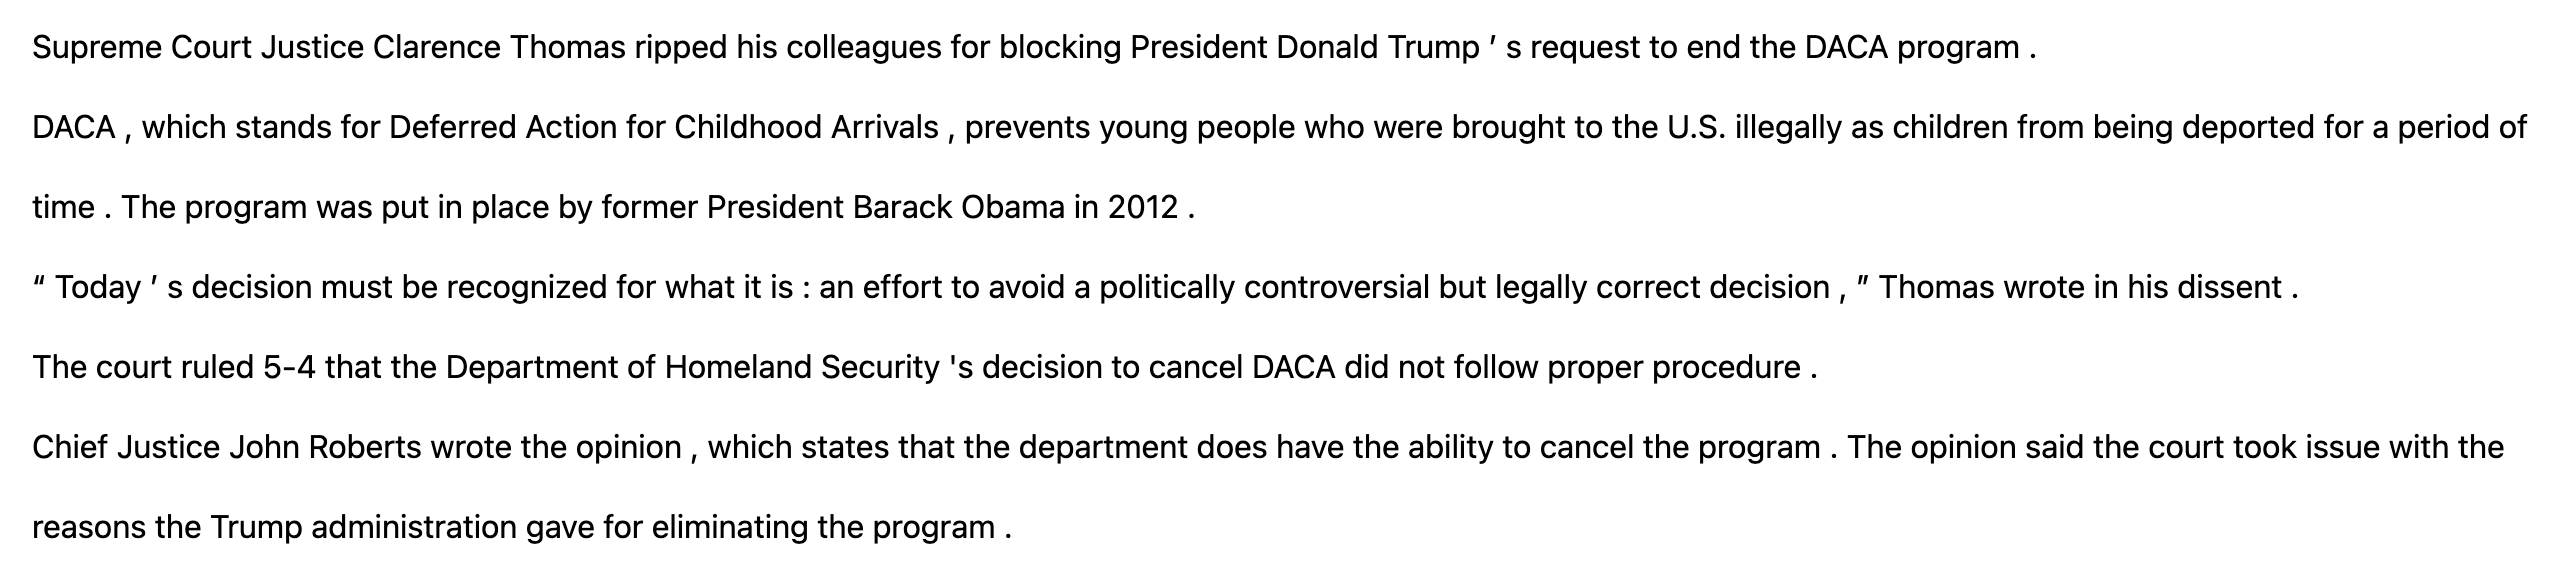
\includegraphics[width=\textwidth]{figures/article_topic_example.png}}
		\caption{Text} % subcaption
	\end{subfigure}
	\vspace{1em} % here you can insert horizontal or vertical space
	\begin{subfigure}{0.45\textwidth} % width of right subfigure
		\centering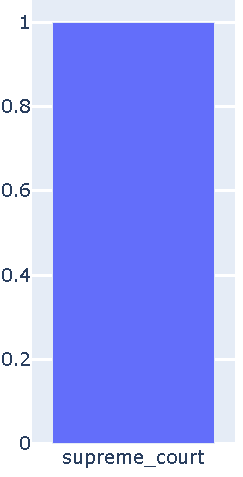
\includegraphics[width=0.29\textwidth]{figures/baly_topics.pdf}
		\caption{Native Baly topic} % subcaption
            \label{fig:topic_analysis_different_tools_baly} 
	\end{subfigure}
	\begin{subfigure}{0.45\textwidth} % width of right subfigure
		\centering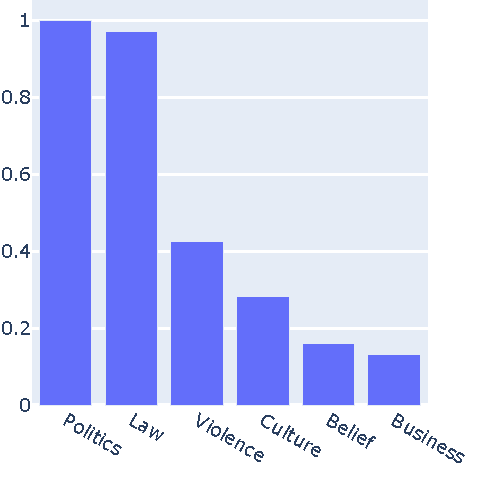
\includegraphics[width=0.6\textwidth]{figures/coarse_topics.pdf}
		\caption{Coarse Topics} % subcaption
            \label{fig:topic_analysis_different_tools_coarse} 
	\end{subfigure}
	\begin{subfigure}{\textwidth} % width of right subfigure
		\centering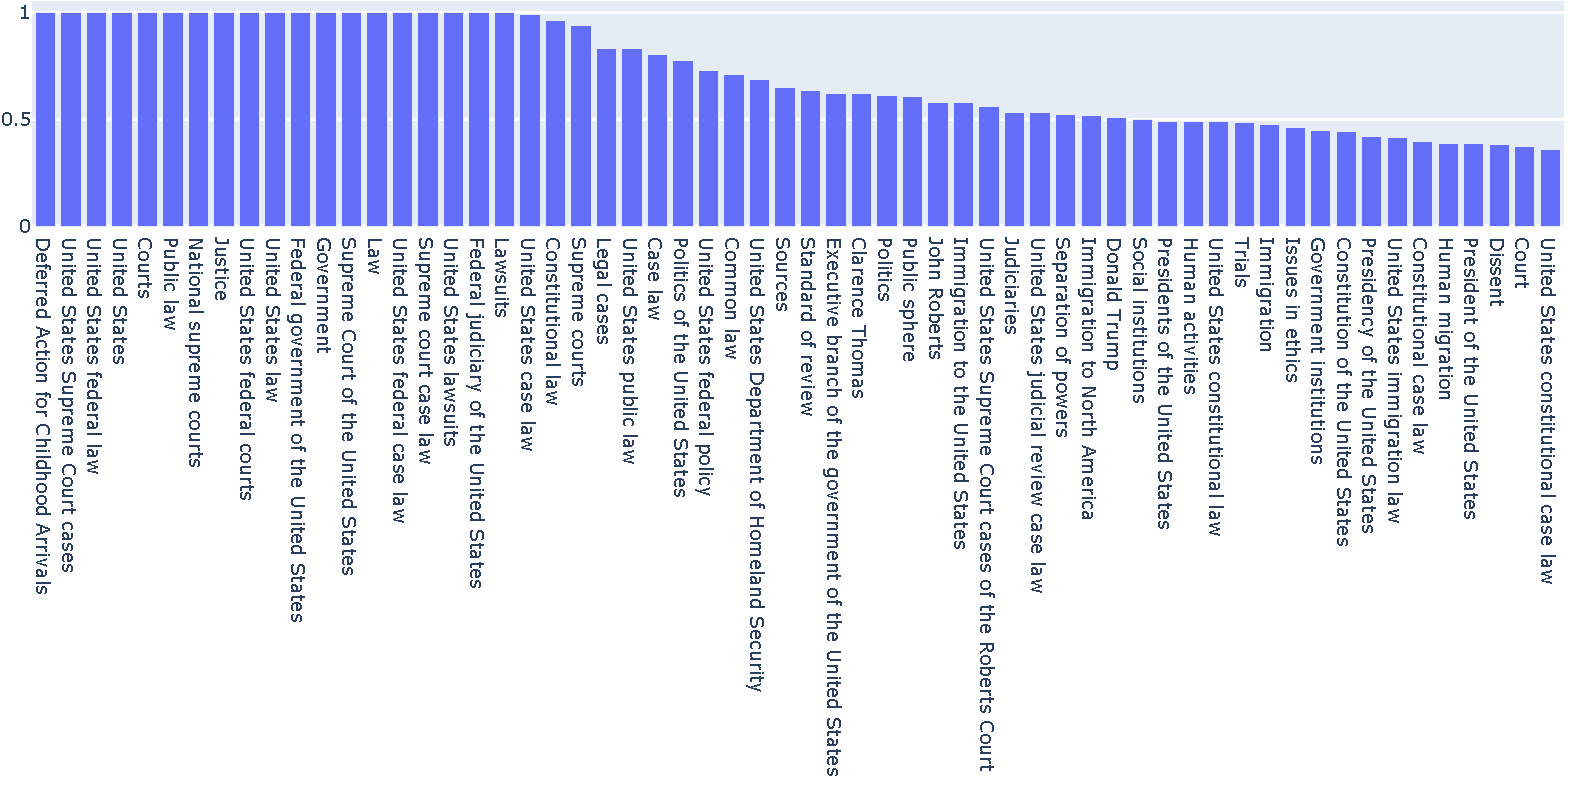
\includegraphics[width=0.7\textwidth]{figures/finegrained_topics.pdf}
		\caption{60 top Fine-grained topics} % subcaption
            \label{fig:topic_analysis_different_tools_fine} 
	\end{subfigure}
	\begin{subfigure}{\textwidth} % width of right subfigure
		\centering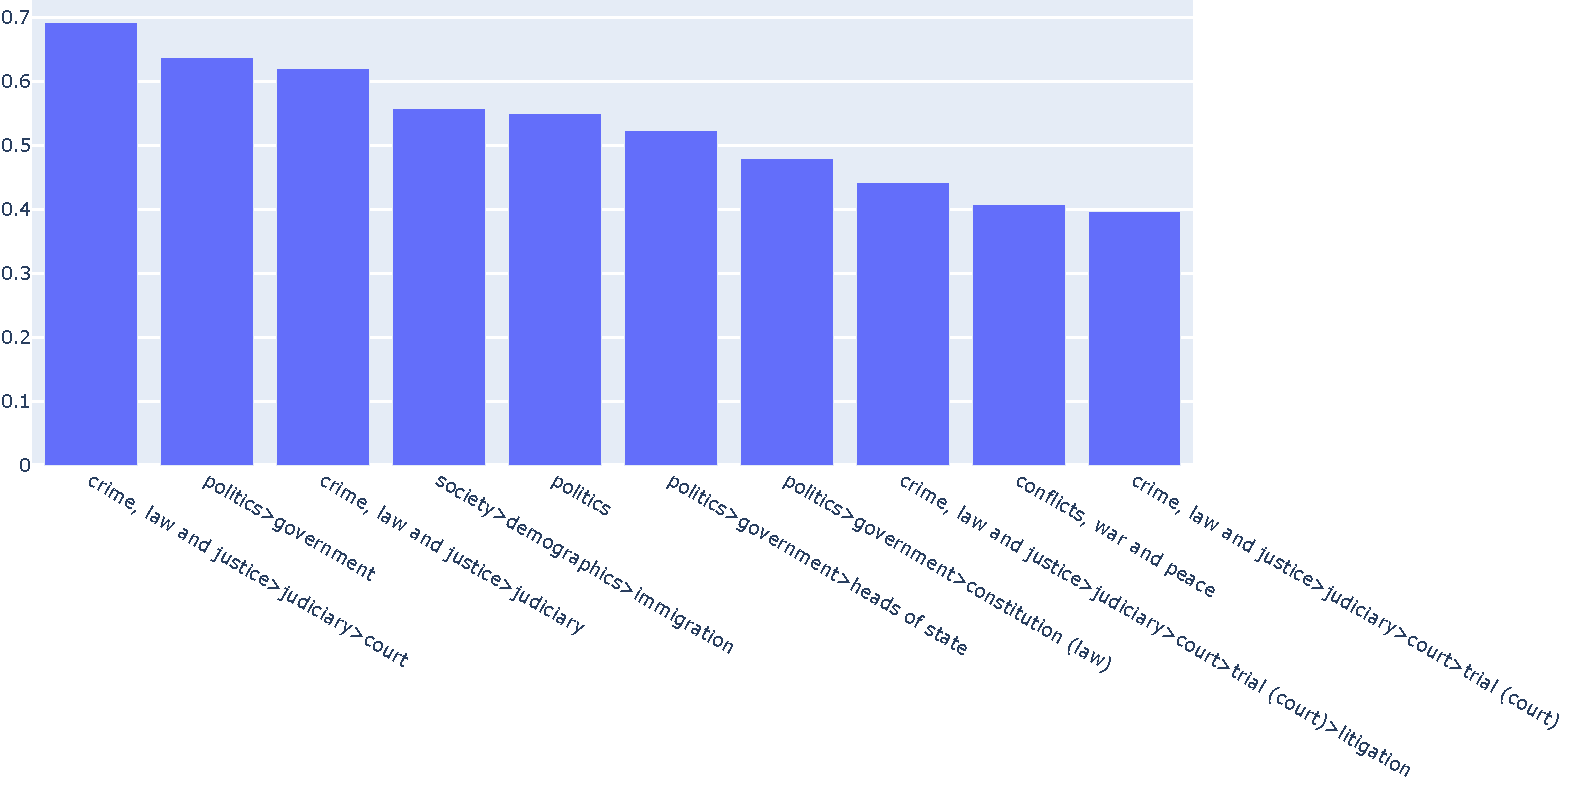
\includegraphics[width=0.7\textwidth]{figures/mediatopics.pdf}
		\caption{Media Topics} % subcaption
            \label{fig:topic_analysis_different_tools_mediatopics} 
	\end{subfigure}
    \caption{Different topic analyses for an example document}
    \label{fig:topic_analysis_different_tools} 
\end{figure}
%\todoAW{Axis labels on all plots}

Figure~\ref{fig:topic_analysis_different_tools} shows an example of these features for an article.\footnote{\url{https://www.newsmax.com/politics/clarence-thomas-daca-illegal-immigrants-dhs/2020/06/18/id/972897/}}
On the vertical axes, we have the topic weights given by the corresponding annotation method, while on the horizontal axis we have the topic labels.
The native topic annotations provided by the dataset (\ref{fig:topic_analysis_different_tools_baly}) have a single topic (\texttt{supreme court}), which is a non-standardised topic.
% These annotations from the dataset suffer from undefined granularity (it is not stated how coarse each topic is, there are wide topics e.g., politics, together with very narrow ones) and undefined enumeration (it is unclear the set of possible labels, not a clear list defined in advance).
%\todoAW{? Not sure what you're getting at here.}
%
Instead the other sub-figures provide the different fuzzy topic annotations from TextRazor.
We have the coarse topics (\ref{fig:topic_analysis_different_tools_coarse}), which are 6 topics that are very broad. Then the fine-grained topics (\ref{fig:topic_analysis_different_tools_fine}), that here we only display the top 60, but there are 270 for this article.
Finally, the Media Topics (\ref{fig:topic_analysis_different_tools_mediatopics}), which are up to 10 for each article, and they are part of a taxonomy.  Therefore, we can see how specific they are and what the parent topics are.

% , but in this chapter we focus on the results given by TextRazor.
% TextRazor gives topics in different ways:

In Sections~\ref{sec:topic_topic_granularities} we use the selected methods to provide statistics of the \texttt{baly} dataset across topics (\ref{ssec:topic_topic_granularities_alone}) and across leanings (\ref{ssec:topics_topics_leaning}). In this way, we also give an insight into the methods themselves and decide which of the methods is better for our comparative analysis.

% \subsection{\statusorange Combining the analysis of dimensions}
\subsection{\statusgreen Comparative Analysis}
\label{sec:topic_method_comparative}

Having the annotations related to three different dimensions (propaganda, leaning and topic), the next step is to perform a comparative analysis bringing the dimensions together.

In the many comparative analyses contained in the following sections, we always have one observed variable (the objective of the analysis) and one or many partitioning variables (the variables that are used to partition the space of the articles of the dataset). The observed variable is an aggregate value computed over the partitions identified by the partitioning variable(s).

\begin{table}[!htbp]
    \centering
    \resizebox{\textwidth}{!}{
    \begin{tabular}{c|c|c}
        Observed variable & Partitioning variables & Section  \\
        \hline
        \#articles & Topics (many definitions) & \ref{ssec:topic_topic_granularities_alone} \\
        \#articles & Topics (many definitions) + Leaning & \ref{ssec:topics_topics_leaning} \\
        Total quantity of propaganda & Topics & \ref{ssec:topic_propaganda_tot} \\
        Quantity of propaganda techniques & Topics + Propaganda Techniques & \ref{ssec:topic_propaganda_tech} \\
        Total quantity of propaganda & Topics + Leaning & \ref{ssec:topic_propaganda_leaning_tot_quantity} \\
        Quantity of propaganda techniques & Topics + Leaning + Propaganda Techniques & \ref{ssec:topic_propaganda_leaning_tech_quantities} \\
        Terms of Propaganda & Topics + Leaning & \ref{ssec:topic_propaganda_leaning_terms} \\
    \end{tabular}
    }
    \caption{The comparative analyses of this chapter}
    \label{tab:comparative_analyses}
\end{table}

Table~\ref{tab:comparative_analyses} shows the different combinations of observed and partitioning variables considered across the chapter.
The comparative analysis is then performed by taking the values of the observed variable and comparing it across the partitions.
In the first two comparative analyses, we are observing how the number of articles changes across topics (and leaning). Our goal for these two experiments is to find an optimal definition of the topic which allows the comparative analysis to have enough insights.
Then, with the other analyses, we take the identified definition of the topic and apply it to several partitionings to answer the first two Research Questions of this chapter.



% we compare them to understand what varies between the different topics, combining them gradually with the other two dimensions (propaganda and leaning).


% \subsection{Linking the experiments together}
% \label{sec:topic_method_linking}
% How each of the following experiments is linked together



% For each of the experiments, we combine differently the annotations and analyse their relationship. For the experiments in Sections~\ref{sec:topic_topic_granularities}, \ref{sec:topic_propaganda} and \ref{sec:topic_propaganda_leaning}, we observe the differences when applying different partitioning of the dataset (based on the chosen annotations). For experiment in Section~\ref{sec:topic_classifier_propaganda}, we instead use the annotations of the topic to break down the results of the political leaning classifier of the previous chapter.

% description of each experiment
% TODO: type 1 and type 2, then hierarchically all the experiments

% Topic analysis at different granularities:
% coarse topics, fine-grained, hierarchical. We need hierarchical topic that can go into detail because high-level topics are very broad and distributions are not very meaningful. We need to take a closer look at the details, but as well to understand where these detailed topics stand in the larger picture. (RQ4.1)

% Topic analysis across political spectrum:
% Coarse topics are very similar across political spectrum
% Fine-grained topics are slightly different (quantity, terms). Which ones? They express the choice of details that we discussed in chapter 3

% PROPAGANDA and Topic: only considering hierarchical topics.
% Which topics contain more detected propaganda?
% How detected propaganda varies across topics? 

% Propaganda and Topic and Leaning:
% Which topics have propaganda that differs the most across the spectrum? (Quantities of techniques/terms/) Measured with the correlation of (propaganda features) between Left and Right.
% Do some of the findings clash with the “knowledge of the context”/”what should happen”? These topics may be the problem for propaganda detection
% Political Leaning Classifier with Propaganda features: adding Topic
% Breakdown of F1 measure across topics. Not train/test but just looking at the models trained in the previous chapter and seeing which topics were more easy/difficult to predict. We cannot train a classifier with 50/100 articles.



% \section{Topic analysis}
% \label{sec:topic_topic}

% Why: understand which practical definition of topic is better for our analysis. Granularity, type, ...

% How: First we recall the definition of topic that we gave in Chapter~\ref{sec:lit_topics} and the computational approaches that are mostly used.

% \subsection{Topic definition}
% \label{sec:topic_topic_def}

% What it is:
% - categories / groups 
% - refer to chapter 2 briefly

% How it relates to concepts described in this thesis:
% - headlines, clusters
% - topic and anti-topic layers/words: refer to Chapter~\ref{ssec:lit_layers_of_info}

% \subsection{Computational Approaches}
% \label{sec:topic_topic_computation}

% \todo{Everything here goes in chapter 2}

% Explain here different tools/methods that provide topics/entities

% We have approaches that try to determine the topics without having external knowledge, and approaches that instead an existing taxonomy/list of topics and try to map the input documents to them.

% \subsubsection{LDA topics}

% One of the most common methods to extract topics is to ``automatically detecting them" from the corpus.
% The idea is to learn from the data and by selecting a specific number of output topics, we get them.
% Problem: difficult to extract labels

% The problem of assigning labels: can we really tell what is different about the groups?
% Need to know beforehand how many topics we want in output.
% TODO

% Topic identification is a method for identifying hidden subjects in enormous amounts of text1. It can help you find common themes or keywords that represent the main ideas of a document or a collection of documents. For example, if you have a set of news articles, you can use topic identification to find out what are the most discussed topics among them.

% One of the techniques for topic identification is called Latent Dirichlet Allocation (LDA)12. It is a statistical model that assumes that each document is composed of a mixture of topics, and each topic is composed of a distribution of words. LDA can learn these topics and words from the data without any prior knowledge or labels. LDA can be implemented using Python’s Gensim package1, which provides various tools for natural language processing.

% LDA is a type of topic modeling that uses a latent Dirichlet allocation approach12. Topic modeling is a form of unsupervised learning that can be used for exploring unstructured text data by inferring the relationships that exist between the words in a set of documents23.

% LDA assumes that each document is composed of a mixture of topics, and each topic is composed of a distribution of words13. LDA can discover topics that are hidden (latent) in a set of text documents by inferring possible topics based on the words in the documents34. LDA uses a generative probabilistic model and Dirichlet distributions to achieve this4.

% Another technique for topic identification is called bag-of-words2. It is a simple way to represent text data as a collection of words and their frequencies. Bag-of-words ignores the order and structure of sentences, but it can capture some basic information about the content and vocabulary of a document. Bag-of-words can be used with simple NLP models such as TF-IDF or Naive Bayes to identify topics from texts.


% \subsubsection{Entity Annotators}
% DBPedia spotlight: entity annotation is not very good. It struggles to recognise all the entities in the articles (proof?) → DISCARDED
% BLINK (Facebook): huge (30GB models to fit on RAM), not running on my laptop. On server: no NVIDIA drivers (wants GPU) → DISCARDED
% Spacy-entity-linker https://github.com/egerber/spaCy-entity-linker/ . Not very widely used. → DISCARDED

% Then from entities, need ways to derive the topics by navigating knowledge bases (wikidata in most cases)

% \subsubsection{TextRazor}
% TextRazor: seems more accurate, industrial, FreeBase taxonomy. Each entity is annotated with wikidata id and a list of FreeBase types. Also provides topics and fine-grained topics

% benchmarks? check that it is better than other tools
% % Regarding the validation of TextRazor, I am not aware of a benchmark done to check if it is better than other tools. It was suggested by Harith to use it, and I find that the data it provides is generally quite good (for topics and entities). But this is qualitative, I didn’t do a benchmark or looked up for benchmarks. The assumption was that it’s a commercial product and it should be good.
% some papers that claim to do benchmarks:
% http://giusepperizzo.github.io/publications/Rizzo\_Erp-LREC2014.pdf for the entities
% https://www.linkedin.com/pulse/google-nli-kill-market-linguistic-apis-review-yuri-kitin/ mentioning that TextRazor is useful because it links to Wikipedia/DBPedia

% TextRazor is the only one that provides already hierarchical topics, the other ones always give topics that are not hierarchical or can be made hierarchical with external knowledge (e.g. using DBPedia to navigate broader topics).

% What it provides



\section{\statusgreen Topics for Comparative Analysis}
\label{sec:topic_topic_granularities}

In this section, we use the different topic methodologies listed above, applying them to the \texttt{baly} dataset.
Our goals are:

\begin{enumerate}
    \item analyse the dataset to understand the topic it contains, using different methodologies;
    \item compare the information provided by each methodology and understand what are the advantages of using one or the other;
    \item see which methodologies we can use to find differences between Left and Right. The dataset itself is made of triples of articles, so we expect that the high-level topics will be very similar, while at the fine-grained level we expect some differences.
\end{enumerate}

% Therefore, we divide this section in two main parts: the first one, Subsection~\ref{ssec:topic_topic_granularities_alone}, contains the analysis of the topics of the dataset, with the different methodologies. The second part, Subsection~\ref{ssec:topics_topics_leaning}, contains a comparative analysis of the topics with respect to political leaning.
% \todoAW{I don't think you need this much description of your document. The outline on p157 is fine.}

% We end this section with~\ref{ssec:topic_topic_choice} which recaps and motivates our choice of hierarchical topic methodology for the next sections.

% This contains 3.1 (topic alone) and 3.2 (topic + leaning).
% This section has to support the need for hierarchical topics.
% We want to analyse differences across topics and granularity is required to be able to inspect at different levels.
% Only top-level topics are not good because they don't show good differences.

% Here we take different topic definitions and we try them to show that we need granularity.

\subsection{\statusgreen Detected Topics in the Dataset}
% \subsection{Detected Topics at different granularities}
\label{ssec:topic_topic_granularities_alone}
% ONLY TOPIC
% Why: understand which practical definition of topic is better for our analysis. Granularity, type, ...

% How: First we recall the definition of topic that we gave in Chapter~\ref{sec:lit_topics} and the computational approaches that are mostly used.

% analysis of baly dataset at different granularities

% RQ4.1 (NO): How can we optimise the definition of the topic in order to have enough details? 


% GOAL
Given our goals 1 and 2, we want to compare the information that different methodologies can provide about a selected dataset. Some techniques may be better to provide general information while others may provide very fine-grained topics.
% what
As described in the Methodology section (\ref{sec:topic_method}),
% we consider the \texttt{baly} dataset and
we apply different topic labels:

% In the following paragraphs we consider:

\begin{enumerate}
    \item AllSides topics
    \item Coarse Topics (TextRazor)
    \item Fine-Grained Topics (TextRazor)
    \item Hierarchical Media Topics (TextRazor)
\end{enumerate}

% We start with the definition of topics that is contained in the Baly dataset, and then we use the different topic types that we get from TextRazor, starting with simple ones to get to the more complex.

\subsubsection{\statusgreen Custom Topics (AllSides)}

The first topic definition that we apply is the one that comes directly from the \texttt{baly} dataset. Together with the triples of articles, available from their website, the AllSides headlines have a manual annotation of the topic, which is given by the editors. In this way, on their website, the users can filter by topic and find related information.
Besides being useful for navigating the website, this is a useful label because it is given directly by the resource creators and not assigned externally.
This attribute is then collected in the \texttt{baly} dataset and we have it available.

\begin{figure}[!htbp]
    \centering
    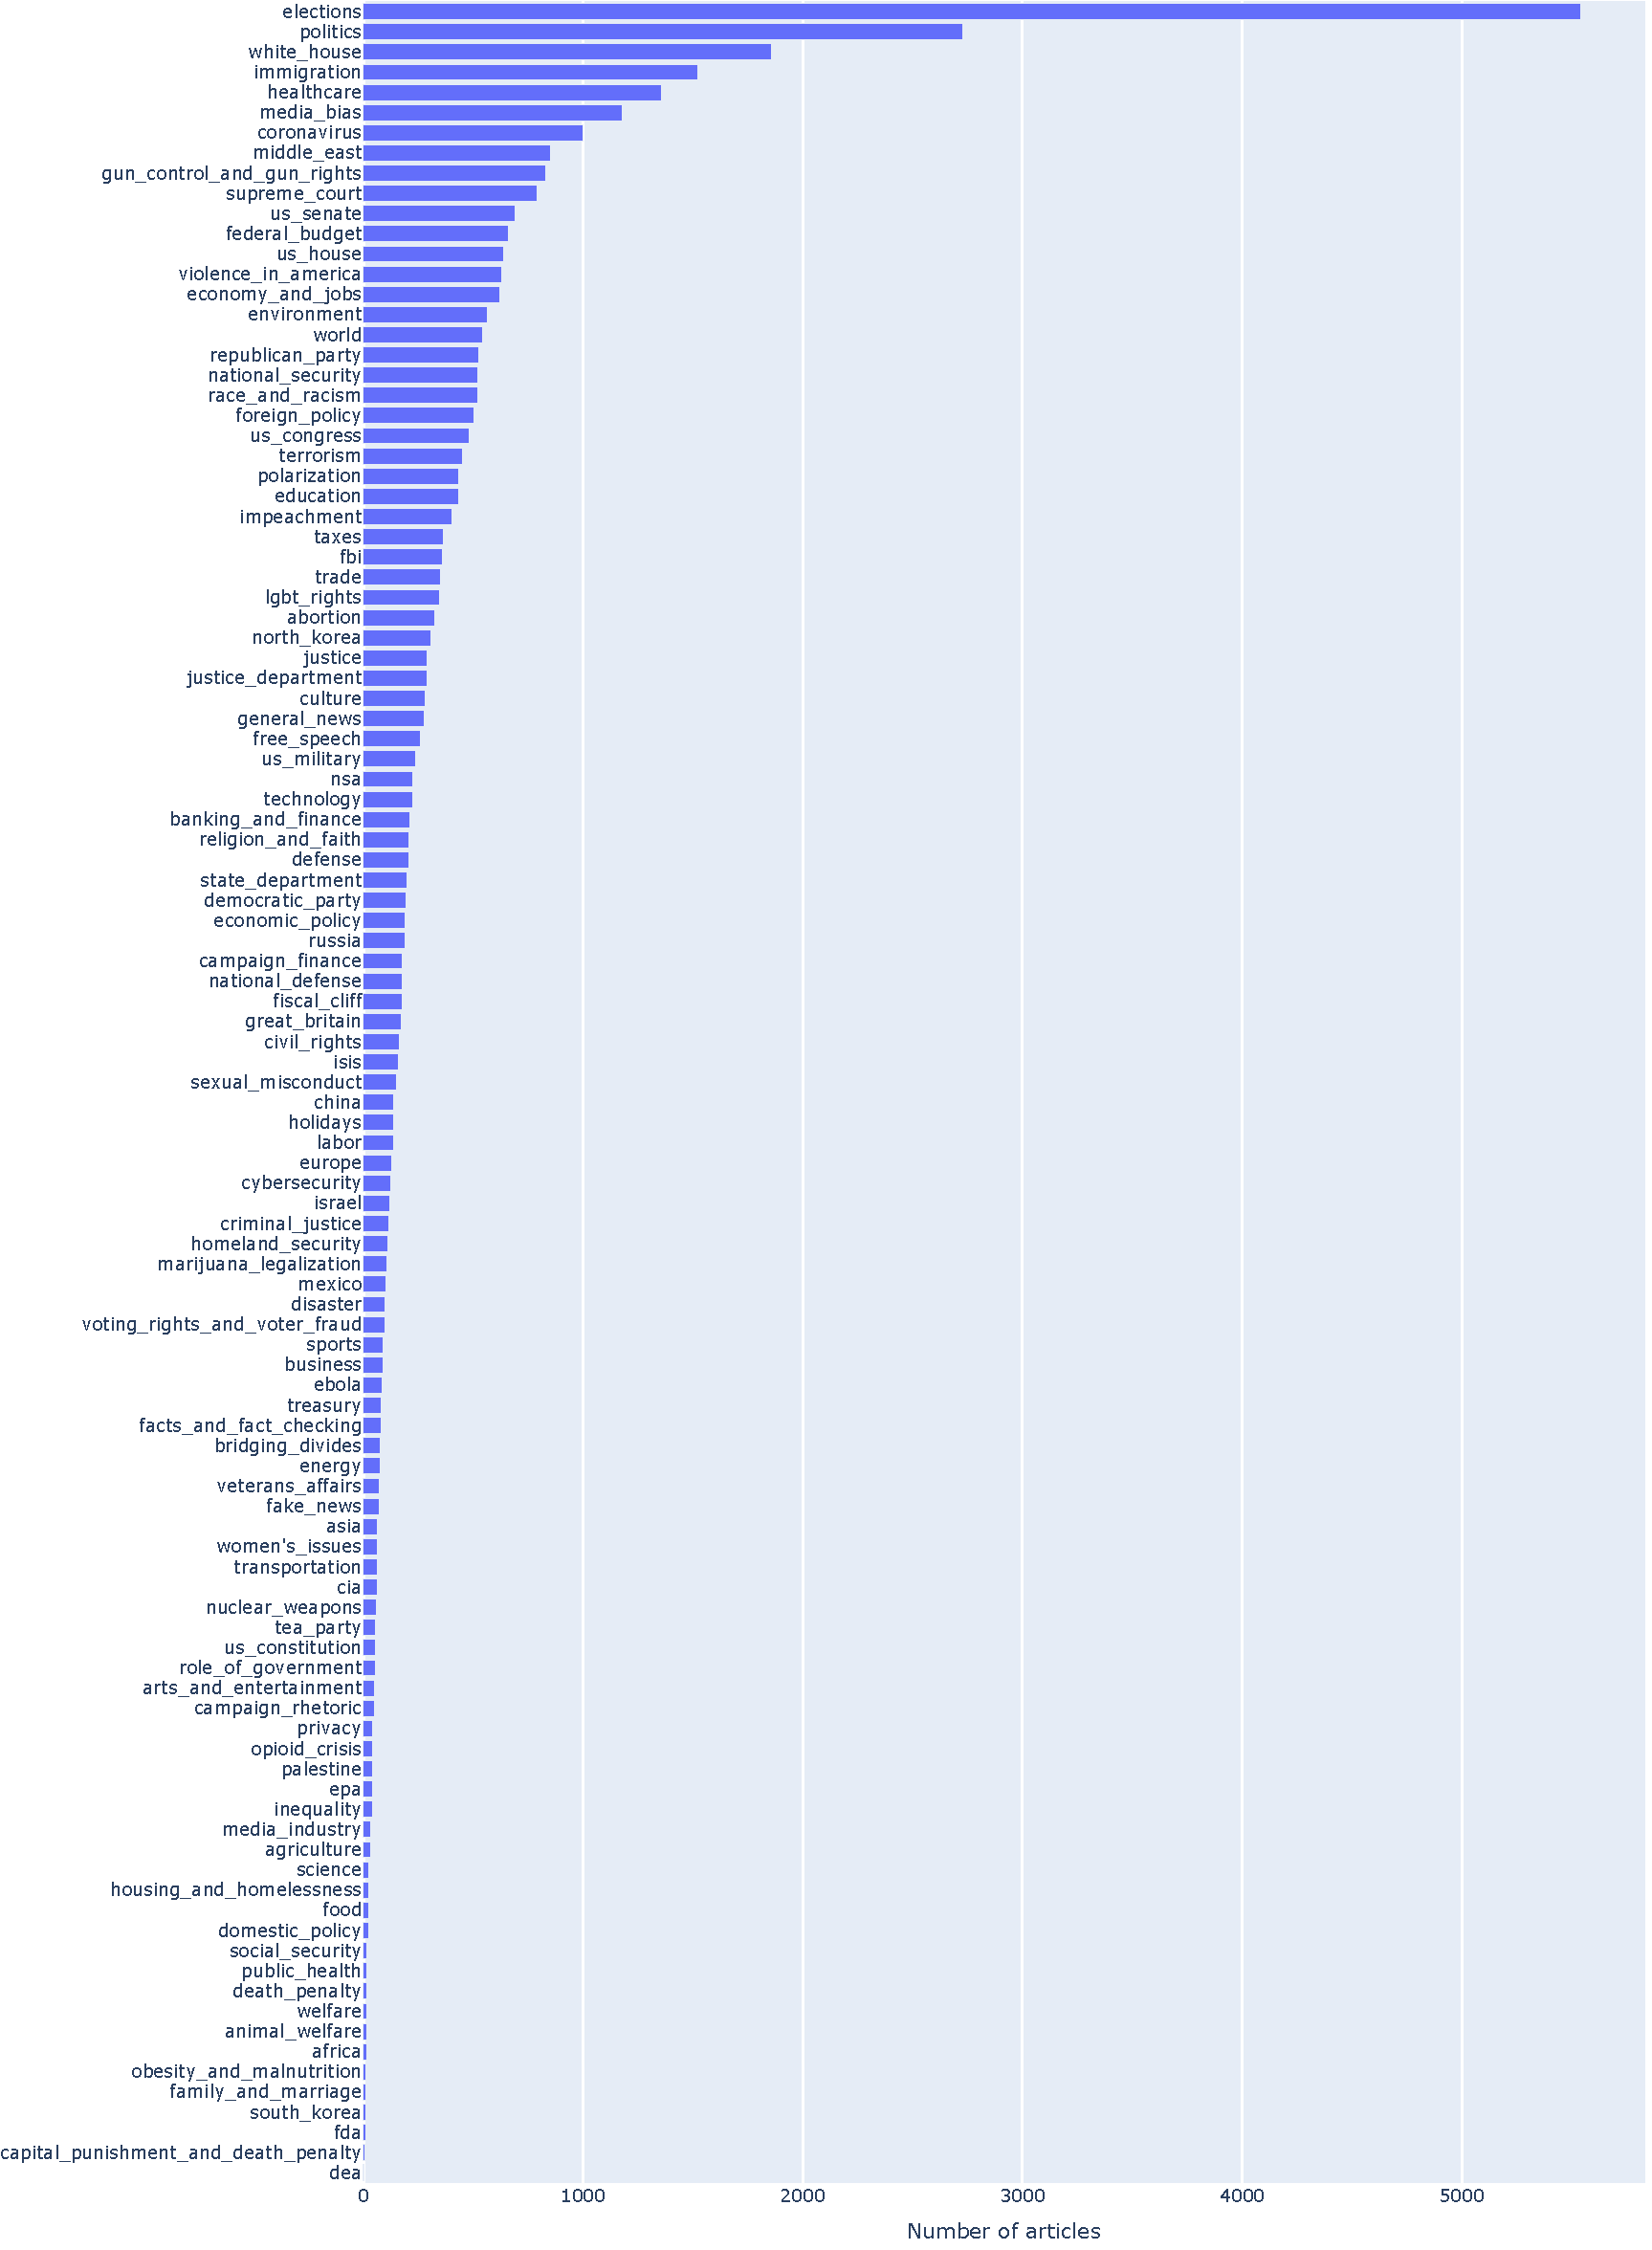
\includegraphics[width=\linewidth]{figures/baly_original_topics.pdf}
    \caption{Original topics of \texttt{Baly} dataset}
    \label{fig:baly_original_topics}
\end{figure}

A complete list of the topics can be found on the AllSides website.\footnote{\url{https://www.allsides.com/topics-issues}}
In Figure~\ref{fig:baly_original_topics}
% \todoHA{From Allsides?!}
% \todomargin{figure is with allsides dataset, but generated by me}
we can see a bar chart of the topics.
On the vertical axis we have the topic labels, and on the horizontal axis we see the number of articles annotated with the corresponding topic.
We can make several observations:

\begin{itemize}
    \item The labels of the topics are not uniform in terms of granularity: there are some very high-level topics (e.g., \texttt{politics}) and some very narrow ones (e.g., \texttt{DEA});
    \item The labels are annotating several aspects and, since there is only one label per article, some articles are annotated for the location mentioned (e.g., \texttt{world}, \texttt{Africa}, \texttt{Russia}, \texttt{Asia}, \texttt{South Korea}) while others for more ubiquitous topics (e.g., \texttt{immigration}, \texttt{healthcare}, \texttt{environment}, \texttt{economic policy}, \texttt{civil rights}); % traversal (food, privacy, healthcare, …)
    \item The distribution is very unbalanced across topics: \texttt{elections} has 5540 articles, while \texttt{DEA} has only 5;
    %\todoAW{A bit too informal: give the precise numbers ("...election has more than XXXX articles, while DEA has only YYY").}
    \item Some topics are subtopics of other ones (e.g. \texttt{elections} is a subtopic of \texttt{politics}) but no information about the relationships is provided;
    \item With 108 flat topics it becomes difficult to compare and organise the topics.
\end{itemize}

An improvement could be done by analysing these labels and manually establishing the relationships, to organise hierarchically the topics.
% \todoAW{Didn't you say that this was already done by IPTC?}
This is not made available with the AllSides topics, but as we will see, the IPTC MediaTopics provide this feature. 
%
% Pro: defined by the authors, by hand
% Cons: hierarchically disomogeneous, highly imbalanced
%
% Original topics
% The dataset is provided together with topic labels but they have a big problem: they are annotated with labels that have very different granularities.
% 108 topic labels
% Most frequent topics: elections, politics (very general), white house, immigration, healthcare
% Least frequent topics: dea, capital punishment and death penalty, fda, south corea
% Labels are not uniform:
% In granularity: e.g., elections vs politics, one is a subtopic of the other
% In aspect: e.g. geography (south corea, africa, china, russia) vs more generic and traversal (food, privacy, healthcare, …)
%
These topic labels are given by the AllSides team with unknown criteria, and the above shows how diverse and not-uniformed they are.
For this reason, the next paragraphs consider standardised topics instead of ad-hoc topics.


\subsubsection{\statusgreen Coarse Topics}

As a next step, we take into consideration the TextRazor Coarse Topics annotations.
TextRazor\footnote{\url{https://www.textrazor.com/}} is a commercial API that allows to analyse topics, entities and to perform other NLP-related tasks (e.g. classify documents).
Regarding the topics, it provides the Coarse Topics, which are 16 very high-level topics (\texttt{Belief}, \texttt{Business}, \texttt{Culture}, \texttt{Education}, \texttt{Health}, \texttt{Language}, \texttt{Law}, \texttt{Leisure}, \texttt{Mathematics}, \texttt{Nature}, \texttt{Politics}, \texttt{Science}, \texttt{Sports}, \texttt{Technology}, \texttt{Violence}, \texttt{Weather}).
Each document is assigned with the top 5/6 matching Coarse Topics, each one with a relevance score which ranges in $[0,1]$. These scores do not sum to $1$. Each document is assigned to multiple topics (multiclass).

For this reason, we explore the topics in two different ways:

\begin{enumerate}
    \item considering the most important topic for each article: this is simpler, each article corresponds to a single topic.
    \item considering the topic weights: each topic corresponds to multiple topics with a specific weight.
\end{enumerate}

\paragraph{Most Relevant Topic Only}

For this first simplification, each article is associated with its most representative topic. This means that if an article is annotated with a score of $1.0$ to Politics and with $0.9$ to Culture, it will only count for Politics because all the topics from the second position onwards are discarded.


\begin{figure}[!htbp]
    \centering
    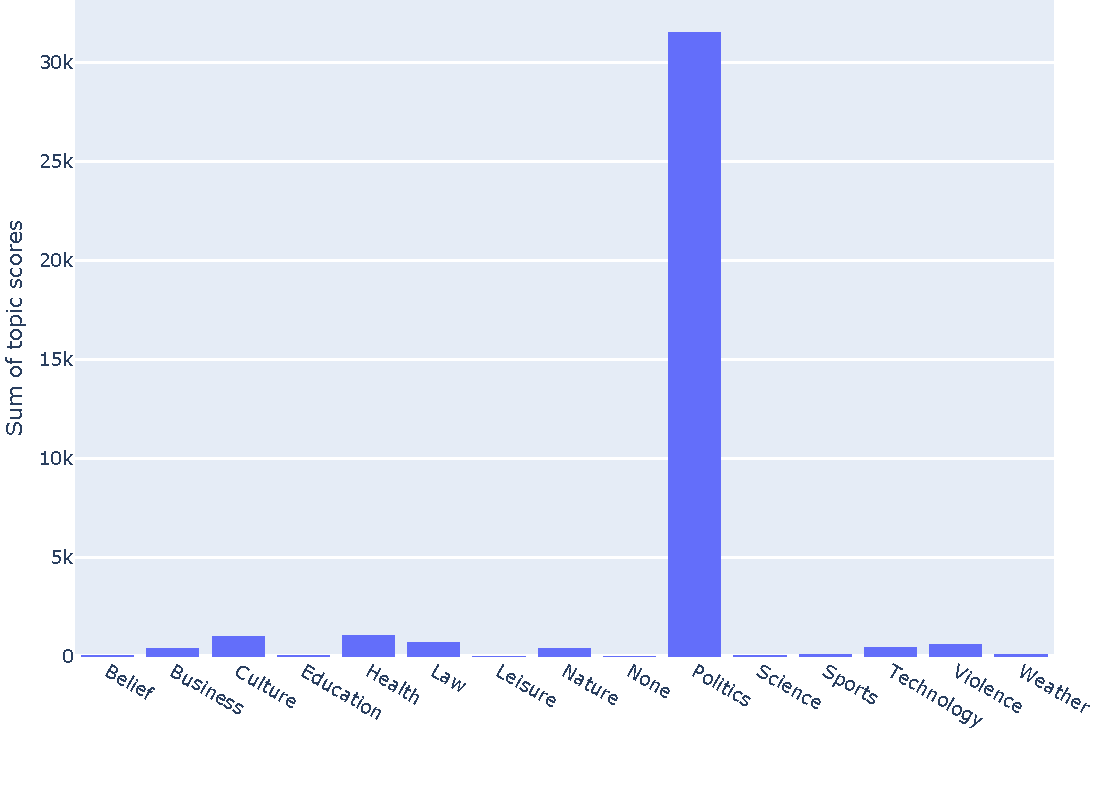
\includegraphics[width=\linewidth]{figures/baly_coarse_first.pdf}
    \caption{Coarse Topics most relevant of \texttt{Baly} dataset}
    \label{fig:baly_coarse_first}
\end{figure}
% \todoAW{ Label your axes!!!}

Figure~\ref{fig:baly_coarse_first} shows on the horizontal axis the 16 topic labels, and on the vertical axis the number of articles that have the corresponding topic as the most relevant, discarding all the labels from the second position onwards.
% We can see how the articles distribute across topics when only considering the most important one.
In this way, the dataset is highly imbalanced towards \texttt{Politics}. This makes this specific usage of the topic annotations highly unusable.

While we can see that the dataset is centred on \texttt{Politics}, the main problem is that all the secondary topics are suppressed.
This plot does not give further insights.
Also, we can see that two of the high-level topics do not even exist in a single article (\texttt{Language} and \texttt{Mathematics}).
This analysis is the result of an oversimplification that is too strong.

\paragraph{Weighted (multi-topic)}

For this reason, we decide to use all the topics for an article and not only the most important one.
If we consider each of the 5/6 topic for each article, we can also see topics which are still very important and may have been discarded only because \texttt{Politics} was slightly higher.

\begin{figure}[!htbp]
    \centering
    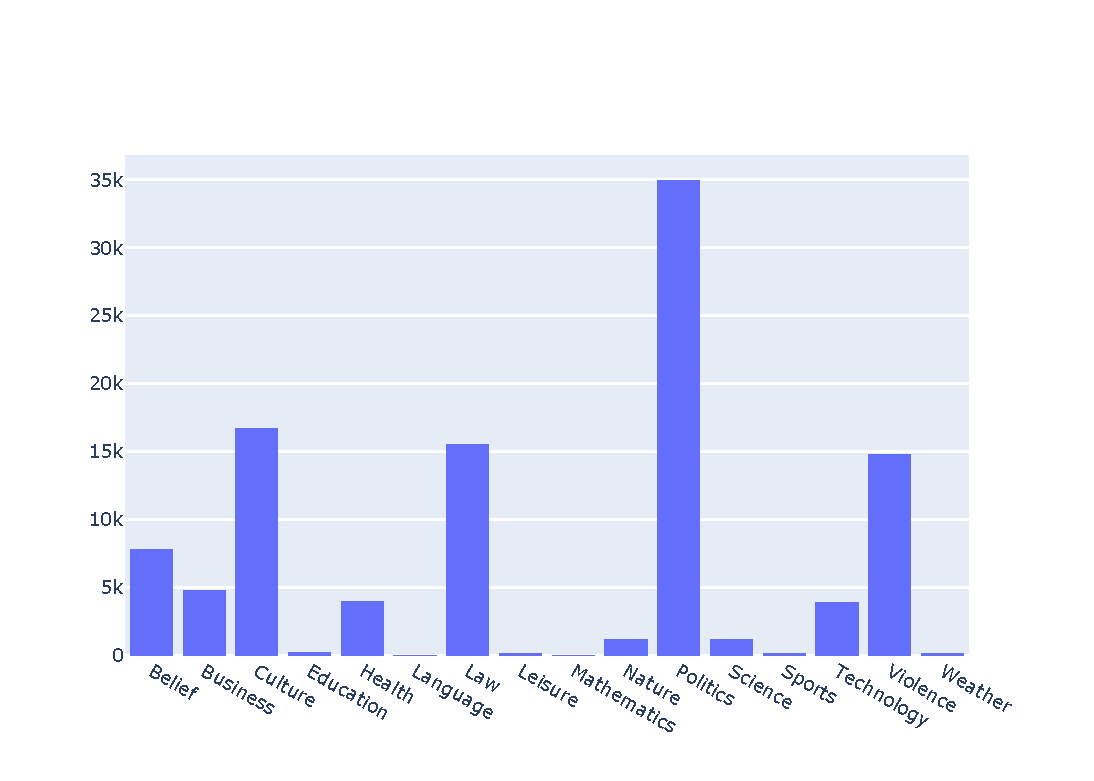
\includegraphics[width=\linewidth]{figures/baly_coarse_weighted.pdf}
    \caption{Coarse Topics weighted of \texttt{Baly} dataset}
    \label{fig:baly_coarse_weighted}
\end{figure}

Figure~\ref{fig:baly_coarse_weighted} has the similar axes as the previous one (horizontal: topics; vertical: sum of the scores of articles for the corresponding topic).
% \todoAW{I can't tell what this diagram is showing, because I don't know what the axes represent.}
In this way we can see that the distribution over topics contains more topics other than \texttt{Politics}.
The most frequent topic across the dataset is still the same, but we can see a big proportion also on secondary topics: \texttt{Culture}, \texttt{Law} and \texttt{Violence}.
%that appear in a significant number of articles.

To produce the values displayed in Figure~\ref{fig:baly_coarse_weighted}, we sum the individual scores given to each article and topic. Being the scores in the $[0,1]$ range, the vertical axis does not represent the number of articles that have a specific topic, but instead represents the sum of the scores. The total number of articles is $37,554$.
%For example, considering that the total number of articles in the dataset is 37,554, we can see that around 35k 

% We can see that the distribution is slightly unbalanced towards politics, then culture, law and violence. This looks like the topics are not too unbalanced, but we have to remember that we would like to have a single document to be categorised only with one topic, and this is not the case.

With respect with the previous Figure~\ref{fig:baly_coarse_first}, we can understand better the topics that the dataset contains.
Still, the topics are very high-level and we have insights about neither which political issues are discussed, nor which subtopics are contained.



% \subsubsection{\statusorange Fine-Grained Topics}

% Moving to the next topic feature, we analyse the annotation that TextRazor provides for Fine-Grained Topics.

% As we saw in subfigure~\ref{fig:topic_analysis_different_tools_fine}, the fine-grained topics are very specific and for each input article, the annotations provide a variable number of them, also some hundreds.
% Fine-grained topics are somewhat similar to mentioned entities, given the high number of matches for each of the articles. Differently from entities, they are not bounded to a specific occurrence in the text (for entities we are able to get the character offsets of the article, to know which words evoke the entities) and an article may contain a fine-grained topic even if the topic name is not  mentioned in the article.

% Across the whole \texttt{baly} dataset, we have $98,504$ distinct fine-grained topics, and it becomes very difficult to present some statistics or graphical representations given this huge number.

% It is good to have fine-grained information that is very specific, but at the same time it is unclear how to link the fine-grained information to the high level topic. What we are missing is some relationship between the two levels, that may possibly be hierarchical with multiple levels.
% With a hierarchy, we can adaptively decide the level of detail and find the optimal one between topics that are too broad (coarse topics for example) and too narrow (fine-grained topics).

% % Baly dataset: 99941 fine-grained topics overall
% % Example:
% % TODO FIGURE MONGO TOPICS

% % annotated only at the article level (not possible to align with propaganda techniques)
% % Many distinct: 98.504
% % At this point maybe we could directly use the entities which have a word-level annotation 


% % find some of them that are specific of a political leaning? 

% \paragraph{\statusred Potential ways to aggregate and find middle-level topics}
% \todo{improve this paragraph}

% To potentially aggregate the topics and find a slightly higher level of hierarchy, there are different solutions.

% The topics have in their attributes the \texttt{wikidata\_id} that is useful to link to Wikidata. Wikidata is useful to see the types of the entity and other relationship types.

% For example, the relationships \texttt{instance\_of} and \texttt{subclass\_of} provide links to wider topics. In theory, every type of relationship is important: e.g. ``Trump Wall" Q61989464 is \texttt{named\_after} Donald Trump.

% Or by using the \texttt{WikiLink}, it is also possible similarly to use the categories tree (in reality it’s a Graph) of Wikipedia.\footnote{ \href{https://en.wikipedia.org/wiki/Special:CategoryTree?target=Category\%3APolitics&mode=all&namespaces=&title=Special\%3ACategoryTree}{https://en.wikipedia.org/wiki/Special:CategoryTree}}

% In both ways, the upper categories are many for each node, and it’s quite difficult to get a clean taxonomy.

% There exist some previous works that addressed this problem.
% cleaning up relationships to extract pages+categories taxonomy.

% WiBi taxonomy → http://wibitaxonomy.org/ dead Wikipedia Bitaxonomy Explorer
% \cite{flati2014wikipedia,flati2014two,ponzetto2009large}

% \cite{chu2019tifi} for fictional domain, cleaning up category graph for fictional domains

% % Backlinks? What are they?

% % Wikipedia categories github experiment? https://github.com/wasiahmad/mining\_wikipedia/tree/master/WikiNomy 



% % Reduction to different granularities of topics:
% % Wikidata IDs → wikidata embeddings? (too difficult, also to explain the features and analysis / explanation)
% % Wikidata ← → link to IPTC topics (offered by IPTC, handmade by them)
% % For each entity, navigate its triples to find IPTC topics. Relationships of type:
% % Instance\_of
% % Subclass\_of
% % ???
% % In theory, every type of relationship is important: e.g. “Trump Wall” Q61989464 is “named after” Donald Trump 


% % Trying to find topics that are not so tight
% % https://en.wikipedia.org/wiki/Wikipedia:Contents/Categories 
% % This number of topics is too high. How to climb a bit up the topic tree in Wikidata?
% % wikidataId → entity. From the entity navigate the relationships instance\_of and subclass\_of. But also other relationships could be useful?
% % From WikiLink → wikipedia page. From the page navigate the categories (recursively) to climb up the categories tree (in reality it’s a Graph) of wikipedia \url{https://en.wikipedia.org/wiki/Special:CategoryTree?target=Category\%3APolitics&mode=all&namespaces=&title=Special%3ACategoryTree}
% % In both ways, the upper categories are many for each node, and it’s quite difficult to get a clean taxonomy.
% % Previous works:
% % https://www.academia.edu/download/30772075/ponzetto\_slides.pdf cleaning up relationships to extract pages+categories taxonomy.
% % https://aclanthology.org/P14-1089.pdf WiBi taxonomy → http://wibitaxonomy.org/ dead http://ceur-ws.org/Vol-1272/paper\_81.pdf https://aclanthology.org/P14-1089.pdf https://www.diag.uniroma1.it/navigli/pubs/IJCAI\_2009\_Ponzetto\_Navigli.pdf 
% % https://dl-acm-org.libezproxy.open.ac.uk/doi/abs/10.1145/3308558.3313519 for fictional domain, cleaning up category graph for fictional domains

% % Backlinks? What are they?

% % Wikipedia categories github experiment? https://github.com/wasiahmad/mining\_wikipedia/tree/master/WikiNomy 
% \paragraph{\statusred A badly structured problem}
% \todo{improve this paragraph}

% Some sentences here, to say that topic taxonomies already exist, and it is better to directly recognise topics using the taxonomies.


% \paragraph{With IPTC}
% So let’s take all the relationships and navigate some hops until an IPTC topic comes up (termination).
% Feature building: decay with the number of hops the weight (exponentially? 1, 0.5, 0.25, …) of each entity.
% Table of entities (quite many distinct), with filter on number of appearances

% \paragraph{Without IPTC}

% We can just take a look at the fine-grained topics:
% Minimum support filter (to reduce features) or select top-k topics

% Option with linked entities:
% Don’t lose a lot of fine-grained topics/entities which don’t have enough support
% Consider them with the related entities in KB
% How to do this: 
% Navigate hops from each entity (decay weight)





% \subsubsection{Derived from Entity types}
% \todo{remove this?}

% Freebase Taxonomy revised by TextRazor

% entity propaganda feature computation
% For each entity, compute the total/average propaganda techniques that co-occur in the same sentence %by each political leaning.
% E.g.: “Donald Trump” used a lot of times with “Doubt” % from the Left leaning.

% Interesting direction:
% With Entity linking (provided by TextRazor) it is possible to find common attributes of the entities that make them targets of %Left/Right 
% propaganda. E.g., a category of people as repeated target of Propaganda

% \paragraph{filter the entities types}

% Using all the entities is too much.

% Option 1: choose the types that will be mostly framed differently by Left/Center/Right (related to politics and sensitive topics e.g. Wikipedia list/ Allsides List
% Option 2: automatically discover the types that are featured more differently from L/C/R in the training dataset

% \paragraph{FreeBase Taxonomy and TextRazor}

% FreeBase vs TextRazor

% Analysis of the types listed in FreeBase
% TextRazor: https://www.textrazor.com/blog/2015/10/freebase-type-deduction-with-data.html they took freebase and are continuing to update it.
% FreeBase build taxonomy: path-like. Let’s build the tree from the path pieces (e.g. /Location/Country is a child of /Location)
% Interesting types: religion, military, law, business, organisation, government, location/country, people (how to justify?)

% Freebase Taxonomy (revised by TextRazor): https://drive.google.com/file/d/145CpFSFA0\_kuzvNt4z\_H1F2nKi-9-YyF/view?usp=sharing 
% Entities types appearing on the headlines dataset: https://drive.google.com/file/d/166fz78O\_xKesnCQ\_hDGiLSH5jk8WdV86/view?usp=sharing 




\subsubsection{\statusgreen IPTC Media Topics}

To solve the problems identified, %(the topics are either too coarse-grained or too fine-grained, without link between them),
we decide to analyse the dataset with a topic taxonomy.
Between the many taxonomies for topics (for specific domains e.g., scientific publications\cite{vayansky2020review,churchill2022evolution}), we focus on the news domain and therefore the most important and used taxonomy is IPTC NewsCodes Media Topics.
This is a taxonomy especially created to describe the topics of news articles. It is made of 17 top-level terms, that can be expanded up to 5 levels of subcategories (total 6 levels).
The full taxonomy can be seen online\footnote{\url{https://cv.iptc.org/newscodes/mediatopic}} and interactively displayed.\footnote{\url{https://show.newscodes.org/index.html?newscodes=medtop&lang=en-GB&startTo=Show}}

% Problem: very difficult to group fine-grained topics into more wide ones
% Solution: IPTC NewsCodes Media Topics schema https://cv.iptc.org/newscodes/mediatopic/
% It’s a taxonomy (6-levels categories)
% TextRazor also provides Media Topics if request is performed with appropriate parameters.

% https://iptc.org/news/wikidata/ 
% TreeView: \url{https://show.newscodes.org/index.html?newscodes=medtop&lang=en-GB&startTo=Show}

% https://cv.iptc.org/newscodes/mediatopic/
% 17 top-level terms
% 5-level taxonomy

TextRazor provides the IPTC Media Topics annotations for submitted texts, if requested with proper parameters.
As we saw in Subfigure~\ref{fig:topic_analysis_different_tools_mediatopics}, each input text is annotated with up to 10 Media Topics (with a weight from 0.0 to 1.0). For each of the Media Topics, it is possible to see the current node and the parent topics up to the top-level topics.
Therefore, it is possible to understand the relationship between the topics and get detailed information but still with the context of which more large topics this belongs to.


% Expecially developed for news
% Hierarchical


% Problem: topic is very unbalanced on this dataset (everything about “politics”)




% IPTC Media Topics
% TextRazor gives in response 10 Media Topics for each article, each one with a score

As in the previous Subsection with Coarse Topics, we consider first a simplified version where only the most relevant Media Topic is taken, and a second version where each article is considered part of several Media Topics.

To represent this, we need to display different types of information:

\begin{itemize}
    \item the \emph{hierarchy}: we want to see results hierarchically, to be able to see both at the coarse level and at the fine-grained level;
    \item the \emph{quantity} of articles belonging to a certain node in the hierarchy of topics: in the previous plots we used bar charts that are very easy to read, but cannot be easily displayed with hierarchical categories;
    \item additionally, present some observed variables for the comparative analysis (e.g., quantity of propaganda, as described in Section~\ref{sec:topic_method_comparative}).
\end{itemize}

For these reasons, when we present the statistics of hierarchical topics, we make use here of icicle diagrams~\cite{kruskal1983icicle}.
They allow to display hierarchical data, and can also be displayed in interactive visualisations, where the user can click to expand the visualisation in a specific area.
However, for a static visualisation they sometimes can present the last levels of granularity with very small nodes, which may be suboptimal.
% Everywhere we use them in this chapter, we truncate the number of levels to 5, even if IPTC Media topics have one layer more.
Furthermore, we create hyperlinks from each plot to an interactive visualisation (reachable by clicking on the figure, and written out in the footnotes), allowing to hover to see the values and click to expand on certain sub-topics.

\paragraph{Most Relevant IPTC Media Topic}

% trim={2.65cm 0cm 2.8cm 0cm},clip,
\begin{figure}[!htbp]
    \centering
    \href{https://martinomensio.github.io/phd-project/figures/baly_iptc_only_first.html}{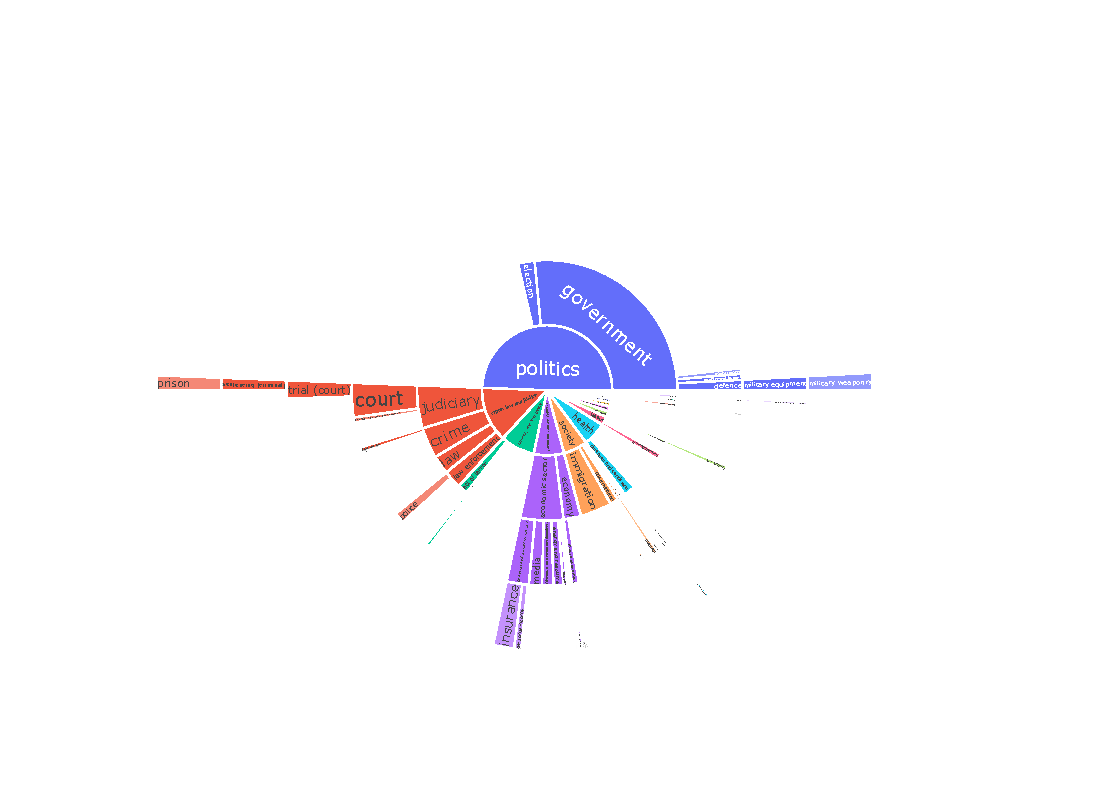
\includegraphics[trim={2.65cm 0cm 0cm 0cm},clip,width=\linewidth]{figures/baly_iptc_only_first.pdf}}
    \caption{IPTC Media Topics of \texttt{Baly} considering only the most important Media Topic for each article}
    \label{fig:baly_iptc_only_first}
\end{figure}
% \todoAW{6.5 vs 6.6 difference, difficult to see on this representation}

For this first simplified version, we consider for each news article only the most important Media Topic (the one with the highest score for each article).

Figure~\ref{fig:baly_iptc_only_first}
% \todoHA{unreadable}
% \todoAW{Wouldn't it make more sense for this to have the same form as figure 6.4?}
shows a icicle diagram\footnote{\url{https://martinomensio.github.io/phd-project/figures/baly_iptc_only_first.html}} that represents how the most relevant topic of each article is distributed across the IPTC Media Topic hierarchy.
On the left, the top-level topics are represented (sorted by size: \texttt{politics}, \texttt{crime-law-and-justice}, \texttt{conflict-war-and-peace}, \texttt{economy-business-and-finance}).
The height of the blocks is proportional to the number of articles that have the specific topic as the primary.
The blocks to the right instead represent subtopics of the ones on the left. For example, \texttt{government} is a subcategory of \texttt{politics}, or \texttt{immigration} is a subcategory of \texttt{society}.

To build this plot, we take the most relevant Media Topic (higher score) and we add its score to the specific node in the tree. Parent nodes also receive the score, since an article that belongs to a certain subtopic also belongs to the corresponding parent topics (up to the top-level topics). The opposite is not true, and this is why summing the size of the subtopics (e.g. \texttt{government} + \texttt{election} + \texttt{government-policy}) the total value is still less than the value for the parent topic (in our case, \texttt{politics}).

% \todoAW{Sunburst diagrams: weird and too many info in the same graph (hierarchy, size, extra info difficult to see relying on color scale). Separate charts, simpler. E.g., p.183 for each technique, show values on separate bar charts (pag 182 for all the techniques, do not skip some). Better maybe bar chart with dendrogram on the bottom? Or nested bar chart? Does it exist?
% If something is interactive, see if it is possible to store it in ORDO permanently (disable CDN libraries)
% }

With respect to the previous figures of this section, we can see not only that \texttt{politics} is the major topic, but we can also get an idea of its main subtopics, as well as very detailed subtopics (6 levels).
However, remembering the difference between Figure~\ref{fig:baly_coarse_first} and \ref{fig:baly_coarse_weighted}, we know that this current plot is a simplification and we need to consider all the Media Topics of each article.
We provided it because it is simpler to explain how the values for the icicle plot are assigned.

% Problem: only politics and government.
% How to solve: when multiple labels are given, avoid the most broad/common ones. E.g.: politics:1.0, politics>elections: 0.85 → choose elections

% What if, instead of trying dirty ways to select only one topic for each article, we keep the multi-topic annotations?
% - Each article instead of having only one topic, is a distribution over a set of topics
% - In the downstream tasks we can use this distribution as the topic description (why should it be only one topic?)
% - If we proceed in this way, we should also do the same analysis with the standard topic distribution (not Media Topics)


\paragraph{Weighted IPTC Media Topics}

By considering all the Media Topics of each article, we have the complete picture of topics of the dataset. 

\begin{figure}[!htbp]
    \centering
    \href{https://martinomensio.github.io/phd-project/figures/baly_iptc_weighted.html}{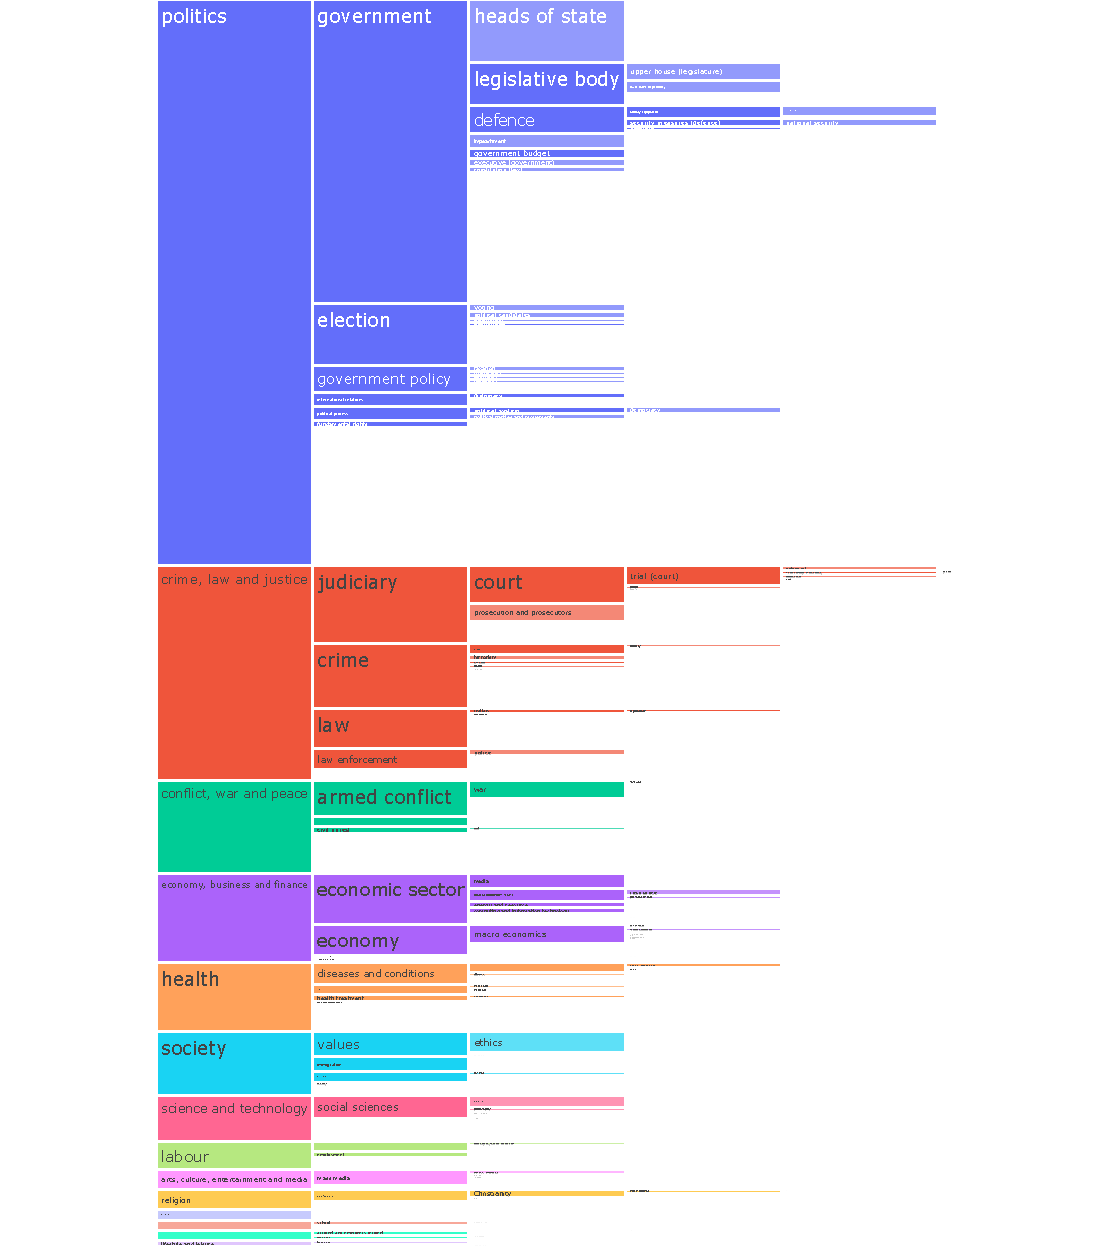
\includegraphics[trim={2.65cm 0cm 0cm 0cm},clip,width=\linewidth]{figures/baly_iptc_weighted.pdf}}
    \caption{IPTC topics weighted of \texttt{Baly} dataset}
    \label{fig:baly_iptc_weighted}
\end{figure}

Figure~\ref{fig:baly_iptc_weighted}
% \todoHA{Also unreadable. Use a bar chart you could add this in an appendix and use a whole page for that}
shows the icicle diagram\footnote{\url{https://martinomensio.github.io/phd-project/figures/baly_iptc_weighted.html}} that is built similarly to the previous case. This time, being each article linked to multiple Media Topics, we can see more subtopics, that were suppressed by the major topic in the previous case (analogously to Fig~\ref{fig:baly_coarse_first} vs Fig~\ref{fig:baly_coarse_weighted}).

For example, under \texttt{government} we see \texttt{legislative-bod}y and \texttt{heads-of-state} that did not appear before. Or \texttt{science-and-technology} and \texttt{economics} that were not visible before.


% Options:
% Multi-topic weighted complex solution
% Only see what happens in specific topic with the classifier
% Input topics as features and see classifier what produces:
% Need to encode the topics hierarchically
% Need model (neural network) on top that can combine the features. Single-layer neural network cannot, need 2 layers at least

% \subsection{Results}

\subsubsection{\statusgreen Comparison}

We have seen in the previous paragraphs several methods and definitions of the topic.

Simple high-level topics show that the majority of articles are about politics. They are able to tell which topics exist, but the labels are very wide and do not provide enough detail.
On the other hand, fine-grained details can be very specific, but it is very difficult to understand how they relate with wider topics.

We analysed two different ways of using multi-class weighted labels. If we consider only the most important topic for each article, we lose a lot of information. Instead, by using all the topics, we are able to see more topics that would be hidden otherwise.

Overall, the method that gives more details and provides a context around the topic (parent topics) is the hierarchical IPTC Media Topics considering all the topics.

We will see in the next subsection how the methods are able to provide a comparative analysis over political leaning.



\subsection{\statusgreen Topic analysis across political spectrum}
\label{ssec:topics_topics_leaning}

Having seen in the previous subsection which level of detail the different topic methodologies are able to provide, we want in this subsection to perform a comparative analysis with respect to political leaning.
We want to observe which topic differences exist across political leaning, using a dataset that is made of triples of articles.
Being groups of three articles that describe the same event, we expect that the high-level topics will be quite similar considering an article from the Left compared with an article from the Right coming from the same triple.
Therefore, also at the dataset level, the statistics at the high-level topics should be quite similar across political leaning.

We would interested in finding some differences when we consider more narrow topics. This would link with our discussion done in Chapter~\ref{chap:common_ground_search} about the choice of details that individual news sources make, covering different subtopics to support their point of view.
Together with the leaning labels (taken from Chapter~\ref{chap:political_sides}) we want to analyse the link between the choice of subtopics and the political orientation of the news sources.

% TOPIC+LEANING: still to support that we need granularity hierarchical topics, other topics are not enough. This time taking the leaning comparison as a first use case and showing evidence that other topics are not useful to do a comparative analysis.

% Coarse topics are very similar across political spectrum
% Fine-grained topics are slightly different (quantity, terms). Which ones? They express the choice of details that we discussed in chapter 3

% RQ4.2: How does the topic (at different granularities) change across political leaning on a parallel news corpus?

We proceed in this subsection by considering the same methodologies for topic labelling as in the previous subsection.

\subsubsection{\statusgreen AllSides topics}

First we use the native topics included in the dataset. We simply count the number of articles for each leaning and topic. Our goal is to see how balanced they are across leaning, and if there are some topics which have more articles on a specific leaninig.

\begin{figure}[!htbp]
    \centering
    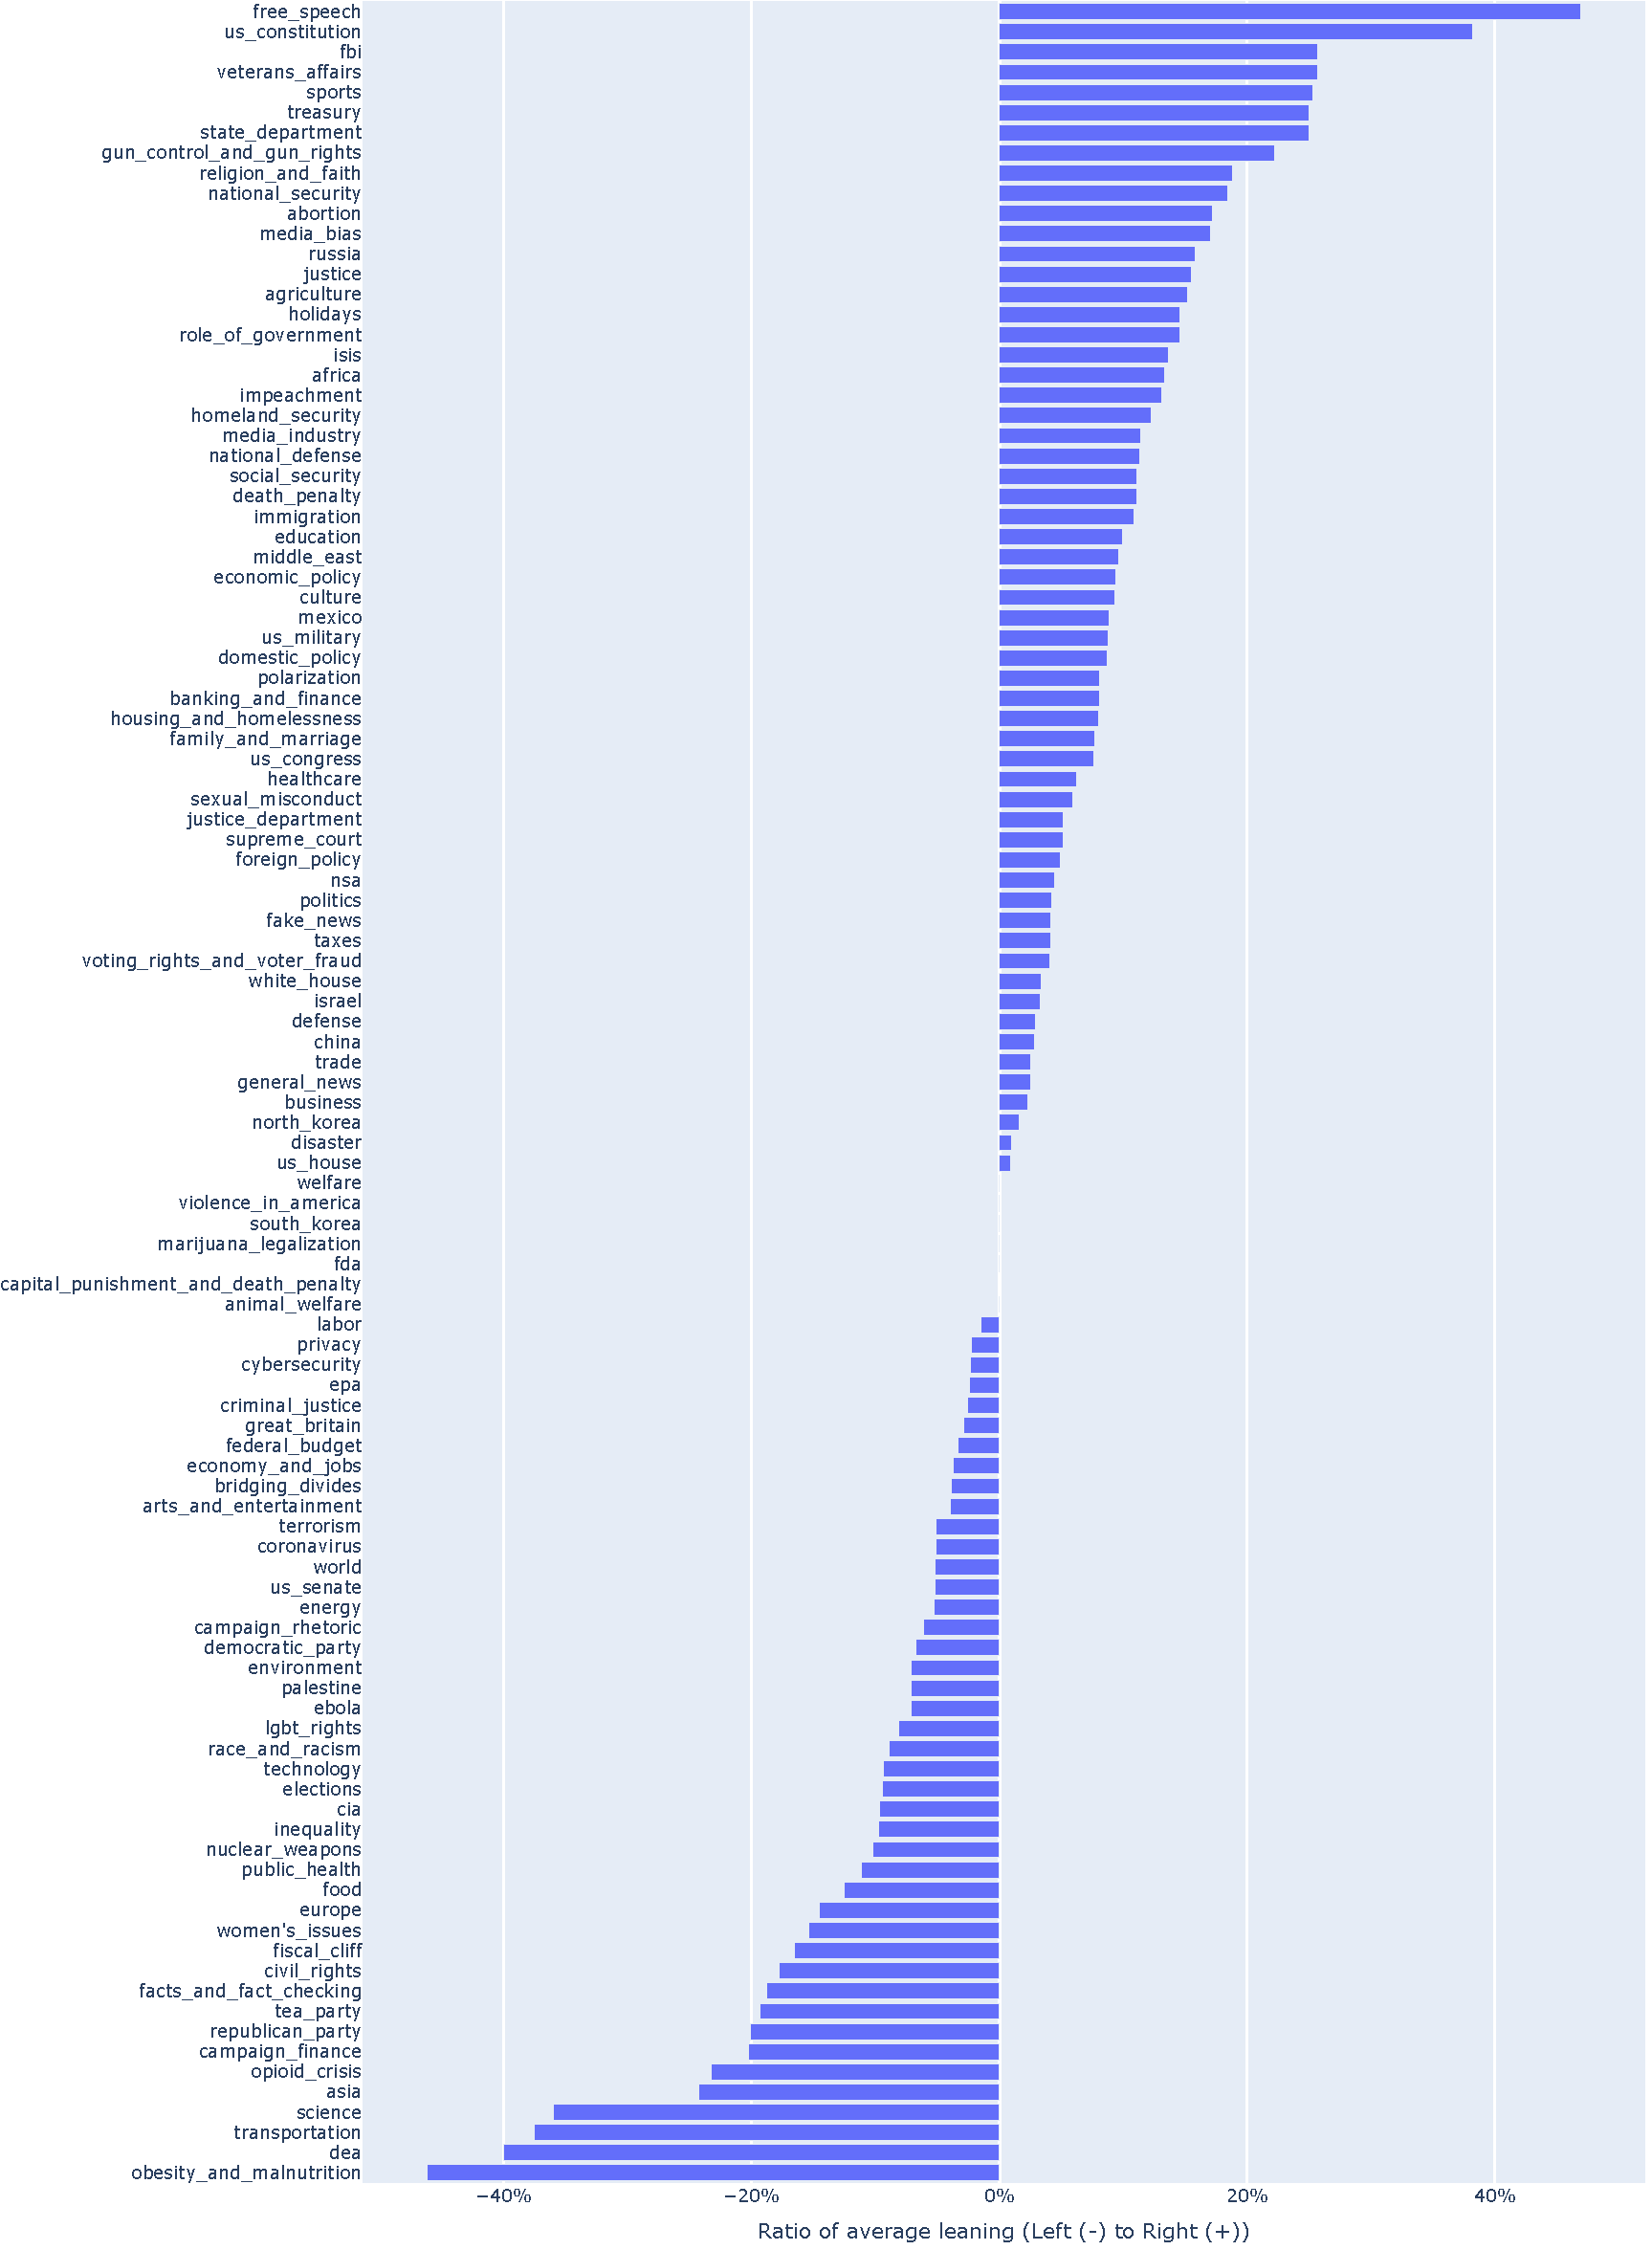
\includegraphics[width=\linewidth]{figures/baly_original_topics_by_leaning_simple.pdf}
    \caption{Average leaning across topics for the \texttt{Baly} dataset}
    \label{fig:baly_original_topics_by_leaning}
\end{figure}
% \todoAW{I can't really read this diagram. You'd be better off isolating the particular cases you mention in the text (lgbt-rights, fbi etc)} \todoHA{?}

In Figure~\ref{fig:baly_original_topics_by_leaning} we show the average leaning for the AllSides topics.
The values are computed as the count of articles belonging to the Right minus the count of the ones of the Left, normalised with the total of articles for the topic.
We can see that for most of the topics
%, the quantity does not change significantly across political leaning.
%But for some topics, we see something unexpected:
there are more articles on a specific leaning. Being the dataset made of triples of articles, we were expecting that everything would have been balanced.
However, the unbalance may be caused by two factors:
\begin{itemize}
    \item some of the triples are made by the AllSides team with unbalanced articles (e.g., two from Left, one from Right);\footnote{\url{https://www.allsides.com/story/greg-craigs-foreign-lobbying-trial-begins}}
    \item during the preparation of the dataset (not available to us) some articles may have been removed because of scraping errors.
\end{itemize}

For example, the topics \texttt{gun-control-and-gun-rights}, \texttt{fbi}, \texttt{free-speech}, \texttt{state-department} has more articles on the Right and fewer in the Center. Instead topics like \texttt{republican-party}, \texttt{lgbt-rights}, \texttt{civil-rights} have more articles on the Left.

This confirms that, even though the AllSides team is trying to maintain the balance by displaying all the sides of the news, the imbalance on such topics is so big that in the end they used two articles from the same leaning.

For such topics, the news coverage is very unbalanced if we consider datasets that do not come from AllSides.
One of the main techniques of agenda setting, is deciding what to cover as news and what to ignore. In this way, the perceived importance of issues is manipulated or diverted~\cite{mccombs1972agenda}.

Besides the positive side of this comparison, we cannot infer from this representation the relationships between the different topics.
We know that \texttt{lgbt-rights} and \texttt{civil-rights} are related, but the flat representation of topics does not provide this information.
Furthermore, some topics are too wide and may internally be imbalanced, while some others are very narrow already.

\subsubsection{\statusgreen Coarse Topics}

Instead of using the AllSides topics, here we use the Coarse Topics from TextRazor, that are very broad but at least they are all at the same level (no detailed topics).

\begin{figure}[!htbp]
    \centering
    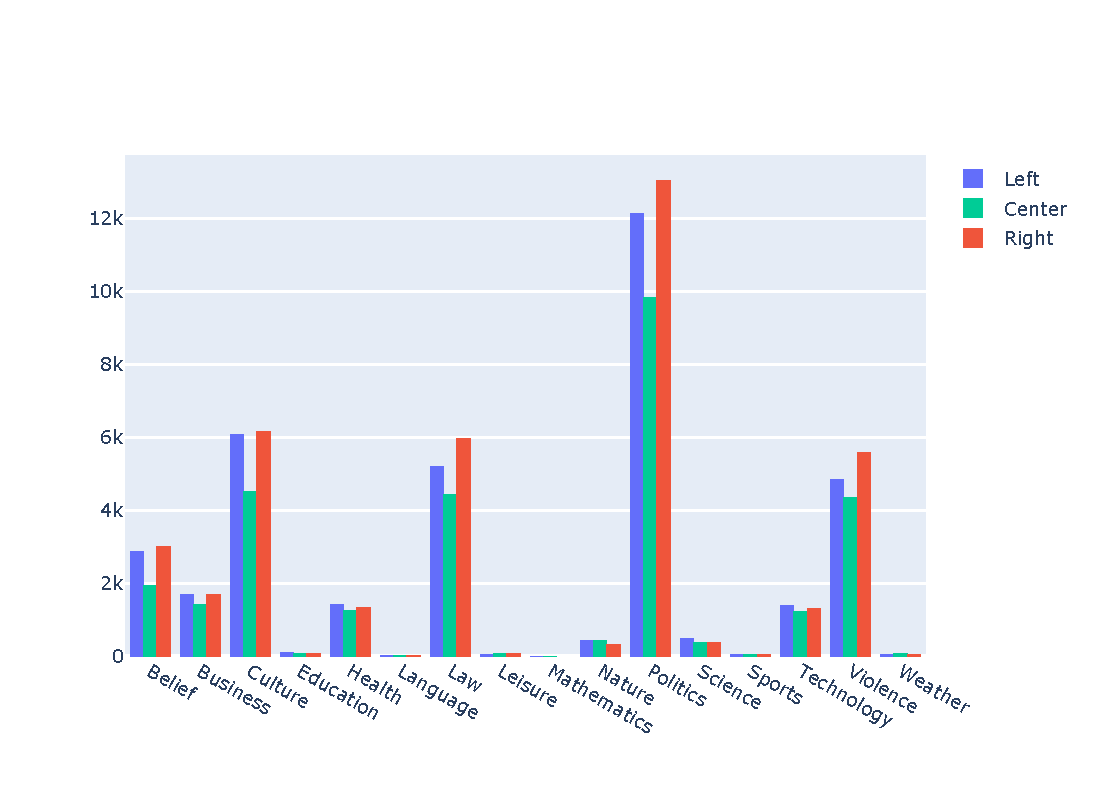
\includegraphics[width=\linewidth]{figures/baly_coarse_weighted_by_leaning.pdf}
    \caption{Coarse Topics weighted of \texttt{Baly} dataset by leaning}
    \label{fig:baly_coarse_weighted_by_leaning}
\end{figure}

Figure~\ref{fig:baly_coarse_weighted_by_leaning} shows the comparison between the different leanings in the dataset with a breakdown by topic.
%
As in the previous plots representing outputs from TextRazor, we are considering the weights given to the topics of each article (score in the $[0,1]$ interval). The Y-axis is the sum of the topic weights across articles.

With respect to the native topics of AllSides, we have that there are less topics (easier to inspect) but also less differences.
While in the previous figure we managed to find several topics with unbalance, here we just see that for some topics there are less articles coming from the Center, and in \texttt{Politics}, \texttt{Violence} and \texttt{Law} there are slightly more articles in the Right than in the Left.

The Coarse Topics are not enough granular to identify the differences across the political spectrum with more details.
%The only difference that we see, is that there are slightly less articles for the Center in all the topics.
%The most prominent topics are Politics, Culture, Law and Violence for all the leanings.
Therefore, we proceed with methods that have more fine-grained topics.

% \subsubsection{\statusred Fine-grained topics}

% By using the Fine-grained topics of TextRazor, we have the problem of high dimensionality. There are too many topics, and it is very difficult to represent them graphically to find the ones that have the most differences.

% \todo{list the top fine-grained topics sorted by support and difference in \% across left-center-right}

% \todo{TF-IDF analysis using topic labels to find if some topic terms are more Left or Right}

% Still we have the problem of not being able to group topics together and find topic groups that are unbalanced.

\subsubsection{\statusgreen IPTC Media Topics}

We have seen with the previous topic definitions that, if we have topics that are detailed enough, we can start to see some differences of unbalance across leaning.

Using the IPTC Media Topics, we want to be able to see such differences, but at the same time have an idea of how the topics relate.
%
% Breaking down with respect to topic, is not helpful to find differences between L/C/R if the topic splitting is very unbalanced and very generic.
% When breaking a dataset of news articles we want to have the possibility to break down the topic enough to see differences. 
We want to discover which topics have an unbalanced coverage between Left and Right. In other words, are there topics that are mostly Left or Right?


\begin{figure}[!htbp]
    \centering
    \href{https://martinomensio.github.io/phd-project/figures/baly_iptc_weighted_by_leaning.html}{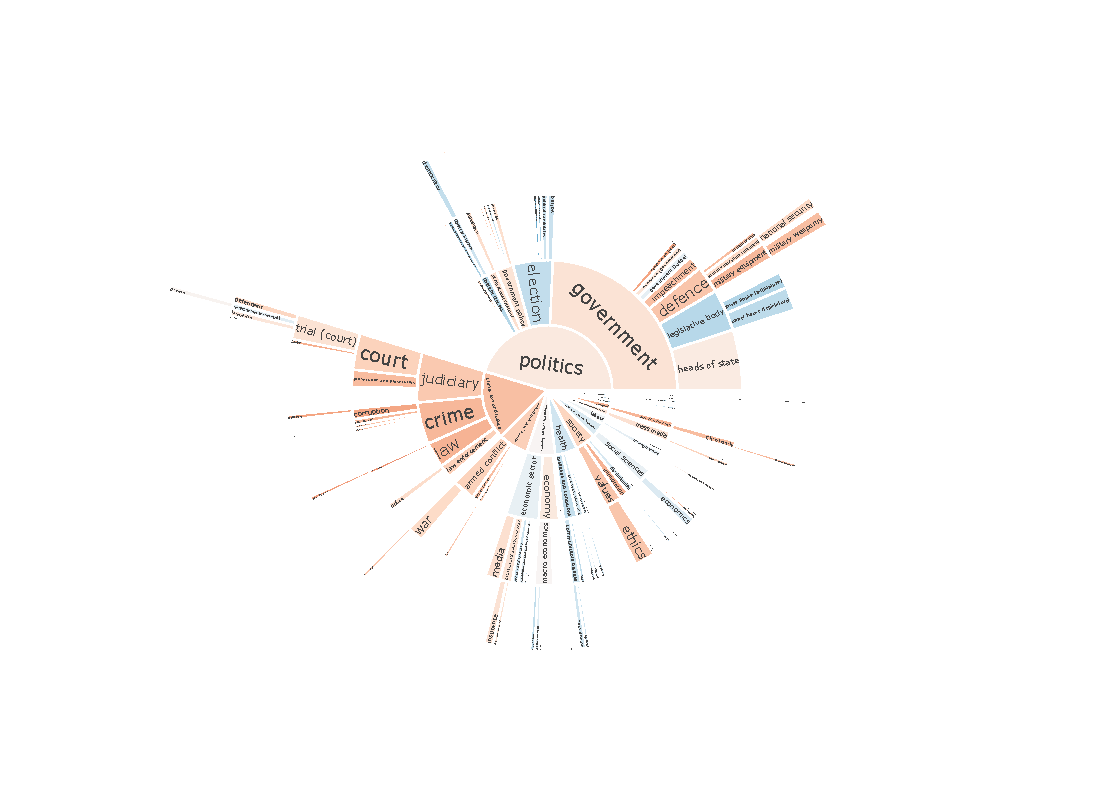
\includegraphics[trim={2.65cm 0cm 0cm 0cm},clip,width=\linewidth]{figures/baly_iptc_weighted_by_leaning.pdf}}
    \caption{IPTC topics weighted of \texttt{Baly} dataset, average leaning (blue=Left, red=Right)}
    \label{fig:baly_iptc_weighted_by_leaning}
\end{figure}

Figure~\ref{fig:baly_iptc_weighted_by_leaning}
% \todoAW{Why do you use the icicle diagram for IPTC, but a stacked bar chart for Allsides?}
shows an icicle diagram where we display the average leaning across the IPTC media topics.\footnote{\url{https://martinomensio.github.io/phd-project/figures/baly_iptc_weighted_by_leaning.html}}
As in the previous diagram of the same type, the height of each node is proportional to the quantity of that topic in the dataset.
Instead, the colour of the edge is computed with the relative proportion of Left and Right. This means that the colours belong to a scale from blue to red, where blue corresponds to Left while red corresponds to Right.

In this way, we can easily see that some topics are covered more by a certain leaning. Furthermore, we have the information about the hierarchy that instead is lost with other types of visualisations.
%
With respect to previous representations, we can see for example that while \texttt{politics} has slightly more articles in the Right ($1\%$), the subtopics of \texttt{elections} and \texttt{legislative-body} instead appear more in the Left ($6\%$ and $8\%$ respectively).


\begin{figure}[!htbp]
    \centering
    \href{https://martinomensio.github.io/phd-project/figures/baly_iptc_weighted_by_leaning.html}{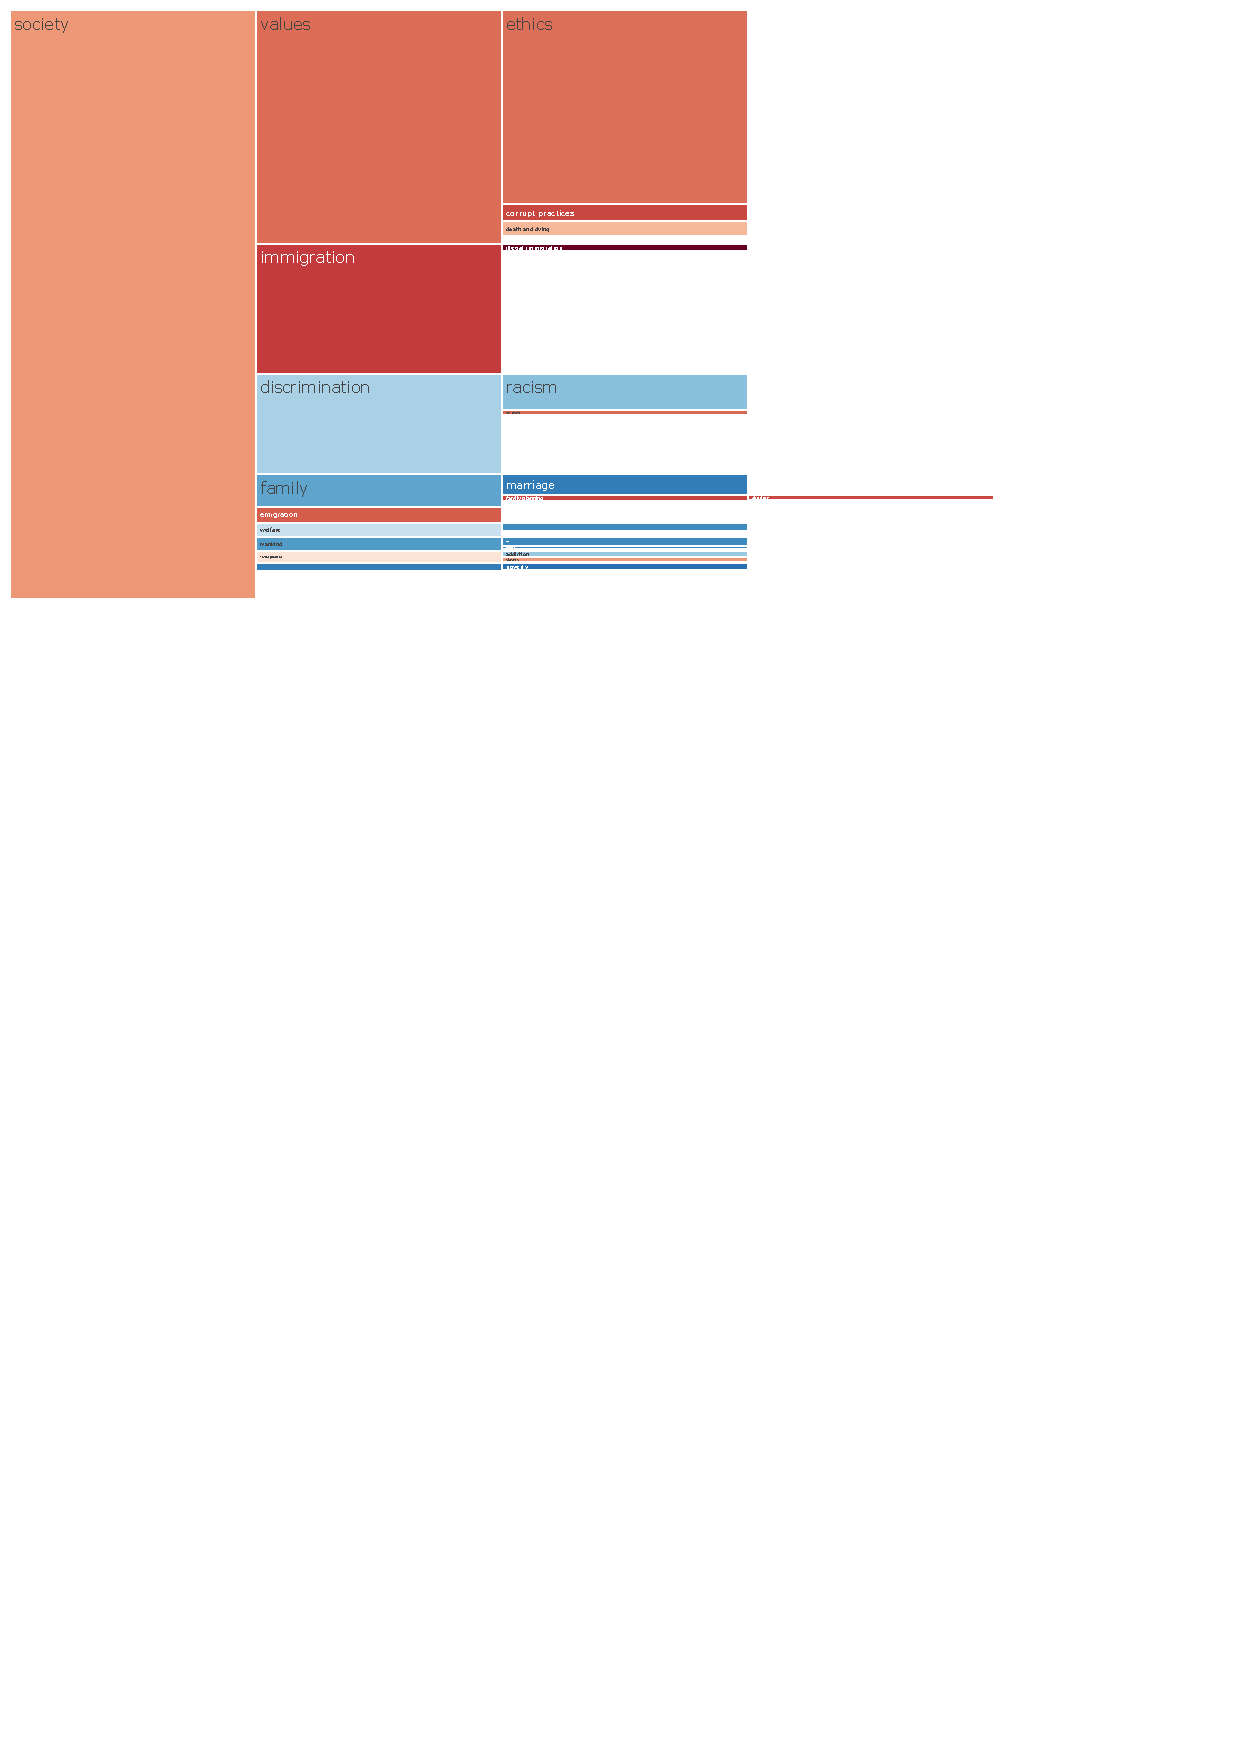
\includegraphics[trim={0.15cm 19.5cm 5cm 0.15cm},clip,width=\linewidth]{figures/baly_iptc_weighted_by_leaning_zoom_society.pdf}}
    \caption{IPTC topics weighted of \texttt{Baly} dataset, average leaning (blue=Left, red=Right), zoom on \texttt{society}.}
    \label{fig:baly_iptc_weighted_by_leaning_zoom_society}
\end{figure}

If we expand on the details of the topic \texttt{society}, we can see how its subtopics are imbalanced in different ways. Figure~\ref{fig:baly_iptc_weighted_by_leaning_zoom_society} shows that \texttt{immigration} and \texttt{values} are covered more by Right leaning ($12\%$ and $8\%$ respectively), while \texttt{discrimination}, \texttt{marriage}
% \todoAW{What does "values" mean here? I'd have thought that marriage was one of the values that the right would discuss.}
and \texttt{LGBTQ} are covered more by the Left ($3\%$, $12\%$ and $10\%$). 

The main findings from this representation is that the Left is more present in \texttt{defence} ($8\%$), \texttt{crime-law-and-justice} ($9\%$), \texttt{religion} ($12\%$) and \texttt{conflict-war-\\and-peace} ($6\%$) topics. Instead the Left is more centred about \texttt{health} ($4\%$), \texttt{economy} ($1\%$), \texttt{science} ($2\%$), \texttt{environment} ($11\%$), and some very specific subtopics of \texttt{politics}.


\subsection{\statusgreen Selected topic methodology}
\label{ssec:topic_topic_choice}

We have seen in the previous subsections several methodologies for defining and extracting the topics from news articles.
We compared the methodologies by first using the topic information on its own (Subsection~\ref{ssec:topic_topic_granularities_alone}), and then in combination with the political leaning (Subsection~\ref{ssec:topics_topics_leaning}).
We have identified our main requirements for our comparative analysis that will consider propaganda, leaning and topic:

\begin{itemize}
    \item fine-grained topics: to be able to identify differences, that at higher levels are not visible;
    \item finite enumeration: know which labels exist, and not have an infinite number of topics;
    \item defined granularity: knowledge of how coarse each topic is; %, there are wide topics, together with very narrow ones
    \item hierarchical topics: to explore the relationships (parent/child) between topics.
\end{itemize}

% Which one
Given these needs, we identified the IPTC Media Topics as ideal candidates.
% Why
They offer fine-grained topics, that are in finite number (see taxonomy). Furthermore, they define the granularity of the topics, and it is possible to navigate the relationships and observe during a comparative analysis.
In the next sections, we will use only the IPTC Media Topics for carrying out our comparative analyses.


\section{\statusgreen Propaganda across Topics}
\label{sec:topic_propaganda}

With respect to the previous sections, from this section onwards we are also considering the propaganda analysis.
As seen in Section~\ref{sec:topic_intro}, the first subquestion (RQ4.1) is addressing Topics and Propaganda:
\emph{How does detected propaganda differ across polarising versus neutral topics?}

To answer this question, we analyse how propaganda is distributed across the topics, to find out which topics contain more propaganda than others (polarising vs non-polarising topics).
We do not take in account political leaning, which is added in the next RQ4.2.
% and what differences topics contain in terms of propaganda.
% Assumption: propaganda is used for certain topics more than in others
We have the following analyses:

\begin{itemize}
    \item analysis of the \emph{total quantity} of propaganda across Media Topics: to discover ones that contain more propaganda (polarising topics) and the ones that instead contain less;
    \item analysis of the \emph{quantity of each propaganda technique} across Media Topics: to discover associations of topics and specific techniques.
    % \item analysis of the terms of propaganda across Media Topics: to discover term associations with specific topics.
\end{itemize}

\subsection{\statusgreen Total quantity of propaganda across Media Topics}
\label{ssec:topic_propaganda_tot}
% \todoAW{all red, change. Proof is in the quantitative analysis. What I want to communicate? Then after change representation}

% one sunburst with total quantity
From the computed features about each article, we consider here the total quantity of propaganda and the Media Topics.
The total quantity of propaganda is a simple percentage that represents the ratio of words that have been annotated as propagandistic by the model presented in~\citet{da2019fine}.
Instead, the Media Topics come in a list with label of the topic and value (interval $[0,1]$).

To compute the average quantity, we iterate over the articles, and for each one of them we see the corresponding propaganda value and the topic values. For each of the topics, we aggregate two different measures: the sum of the topic scores $w_{t_{i},a_{j}}$ (acts as a total counter for that specific topic $t_{i}$ across all the articles $a_{j}$, and is computed as before to create the icicle diagrams), and the propaganda scores multiplied for the topic scores $w_{t_{i},a_{j}} \cdot p_{a_{j}}$ ($p_{a_{j}}$ stands for the quantity of propaganda for article $a_{j}$).
For accounting the hierarchy, we propagate these values from the children nodes to their parent nodes, which are summed together ($i\subseteq k$).
The final average quantity of propaganda for each topic is then computed as:

$$ p_{t_{k}} = \frac{ \sum_{j} \sum_{i\subseteq k} w_{t_{i},a_{j}} \cdot p_{a_{j}} }{ \sum_{j} \sum_{i\subseteq k} w_{t_{i},a_{j}} } $$

\begin{figure}[!htbp]
    \centering
    \href{https://martinomensio.github.io/phd-project/figures/baly_iptc_weighted_prop_total.html}{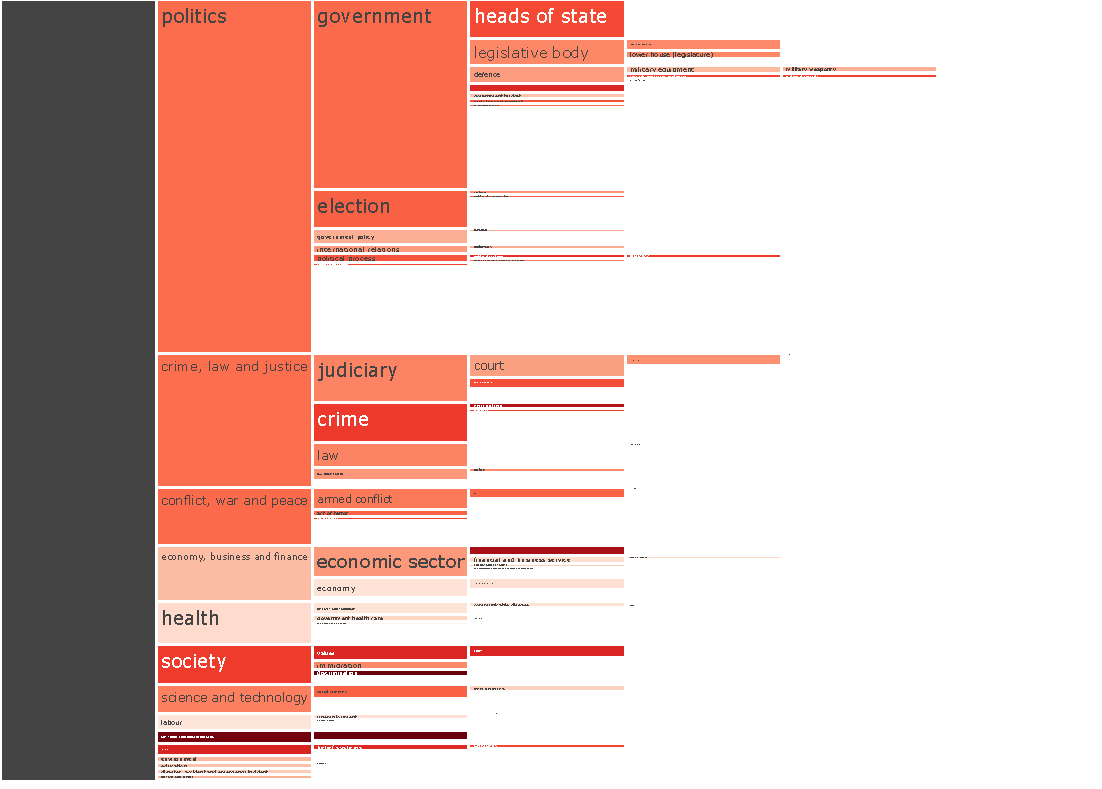
\includegraphics[trim={2.65cm 0cm 0cm 0cm},clip,width=\linewidth]{figures/baly_iptc_weighted_prop_total.pdf}}
    \caption{Total quantity of propaganda across Media Topics}
    \label{fig:baly_iptc_weighted_prop_total}
\end{figure}

Figure~\ref{fig:baly_iptc_weighted_prop_total}
% \todoAW{I don't understand this, and I can't really distinguish between the shades of red.}
shows the total quantity of propaganda across Media Topics on a redscale: dark red means more propaganda, light red means less.\footnote{\url{https://martinomensio.github.io/phd-project/figures/baly_iptc_weighted_prop_total.html}}
The average value is around $5\%$, with the highest just above $10\%$.

The topics with most propaganda are: \texttt{sexism} ($9.9\%$) and \texttt{racism} ($9.1\%$), that are both subtopics of \texttt{discrimination} ($8.1\%$), then \texttt{mass-media} ($8.0\%$) and \texttt{corruption} ($7.2\%$). The lowest values instead are found in \texttt{economy} ($3.5\%$), \texttt{health} ($3.7\%$), \texttt{government-policy} ($4.4\%$) and \texttt{defence} ($4.7\%$).

Although we can already distinguish some loaded/polarising topics, we would also like to see the breakdown by specific techniques, therefore in the next subsection we consider each technique individually.

\subsection{\statusgreen Quantity of each propaganda technique across Media Topics}
\label{ssec:topic_propaganda_tech}

Similarly to what we have done in Chapter~\ref{chap:linguistic_persuasion}, we want to separate the different techniques. Instead of comparing only the total quantity of propaganda across topics, here we want to see how each of the techniques is distributed across the topics. 

Therefore, when we compute the average quantity of propaganda for the topics, we have to differentiate with respect to the specific technique. In the mathematical formulation, we add from the previous case the technique $m_{l}$ where $l$ is an integer between 1 and 18 that identifies the technique:

$$ p_{t_{k},m_{l}} = \frac{ \sum_{j} \sum_{i\subseteq k} w_{t_{i},a_{j}} \cdot p_{a_{j},m_{l}} }{ \sum_{j} \sum_{i\subseteq k} w_{t_{i},a_{j}} } $$


\begin{figure}[!htbp]
    \centering
	\begin{subfigure}{0.45\textwidth}
		\href{https://martinomensio.github.io/phd-project/figures/baly_iptc_weighted_prop_tech.html#Loaded_Language}{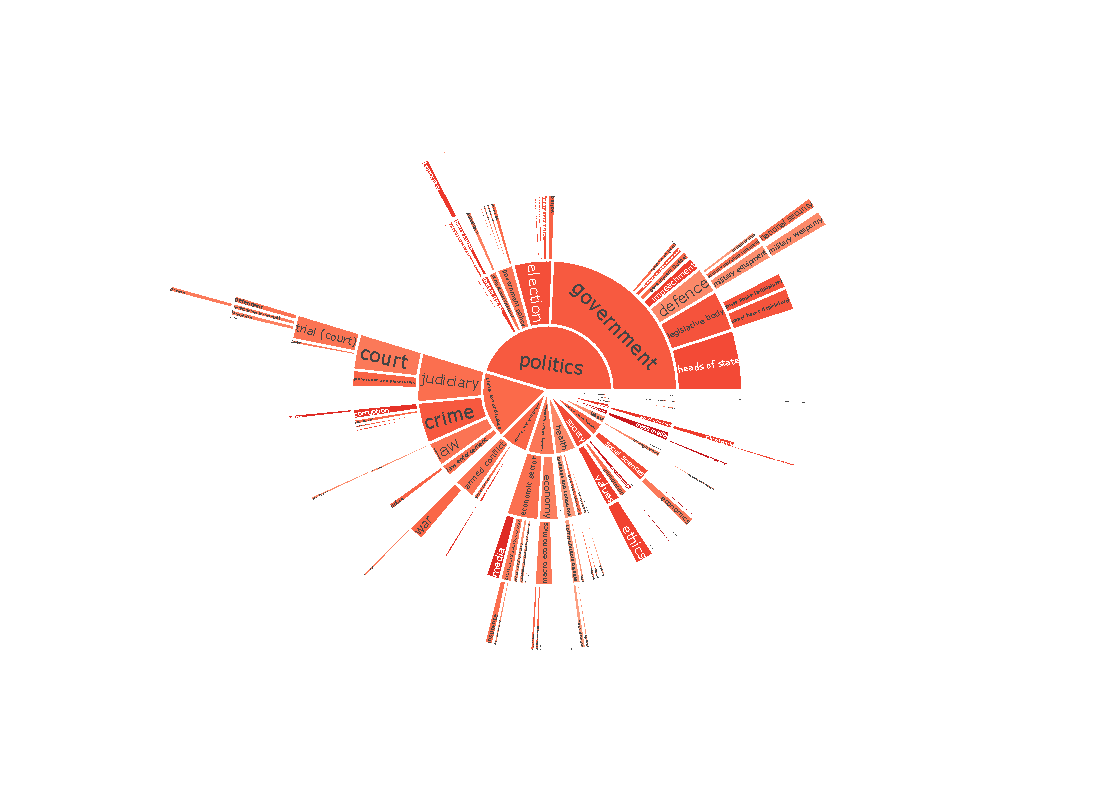
\includegraphics[trim={2.65cm 0cm 0cm 0cm},clip,width=\linewidth]{figures/baly_iptc_weighted_prop_tech_Loaded_Language.pdf}}
		\caption{Loaded Language}
            \label{fig:baly_iptc_weighted_prop_tech_Loaded_Language}
	\end{subfigure}
	\begin{subfigure}{0.45\textwidth}
		\href{https://martinomensio.github.io/phd-project/figures/baly_iptc_weighted_prop_tech.html#Doubt}{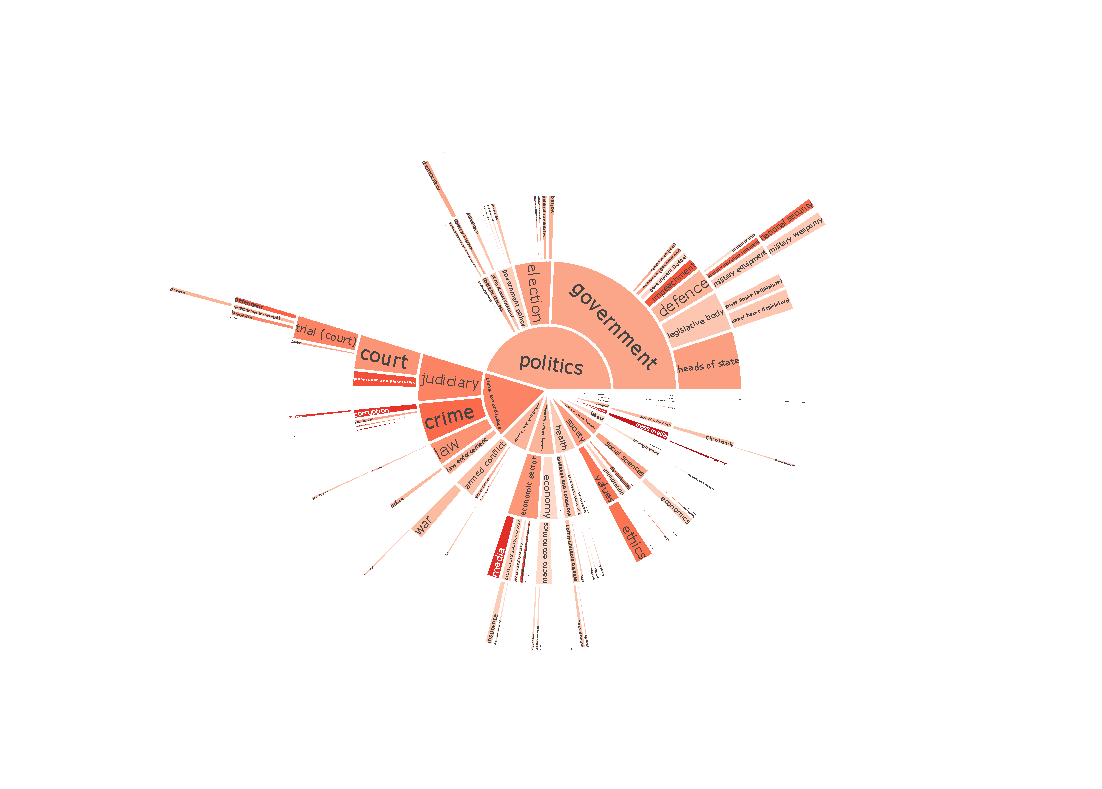
\includegraphics[trim={2.65cm 0cm 0cm 0cm},clip,width=\linewidth]{figures/baly_iptc_weighted_prop_tech_Doubt.pdf}}
		\caption{Doubt}
            \label{fig:baly_iptc_weighted_prop_tech_Doubt}
	\end{subfigure}
	\begin{subfigure}{0.45\textwidth}
		\href{https://martinomensio.github.io/phd-project/figures/baly_iptc_weighted_prop_tech.html#Flag-Waving}{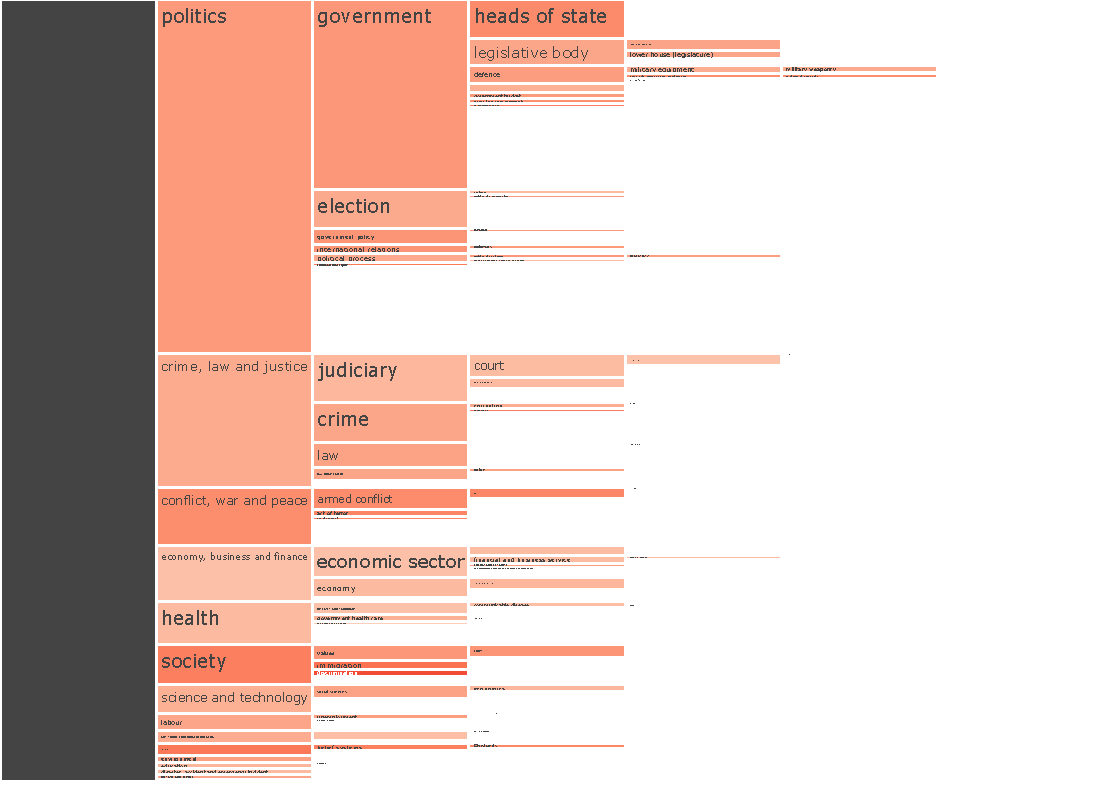
\includegraphics[trim={2.65cm 0cm 0cm 0cm},clip,width=\linewidth]{figures/baly_iptc_weighted_prop_tech_Flag-Waving.pdf}}
		\caption{Flag-Waving}
            \label{fig:baly_iptc_weighted_prop_tech_Flag-Waving}
	\end{subfigure}
	\begin{subfigure}{0.45\textwidth}
		\href{https://martinomensio.github.io/phd-project/figures/baly_iptc_weighted_prop_tech.html#Name_Calling-Labeling}{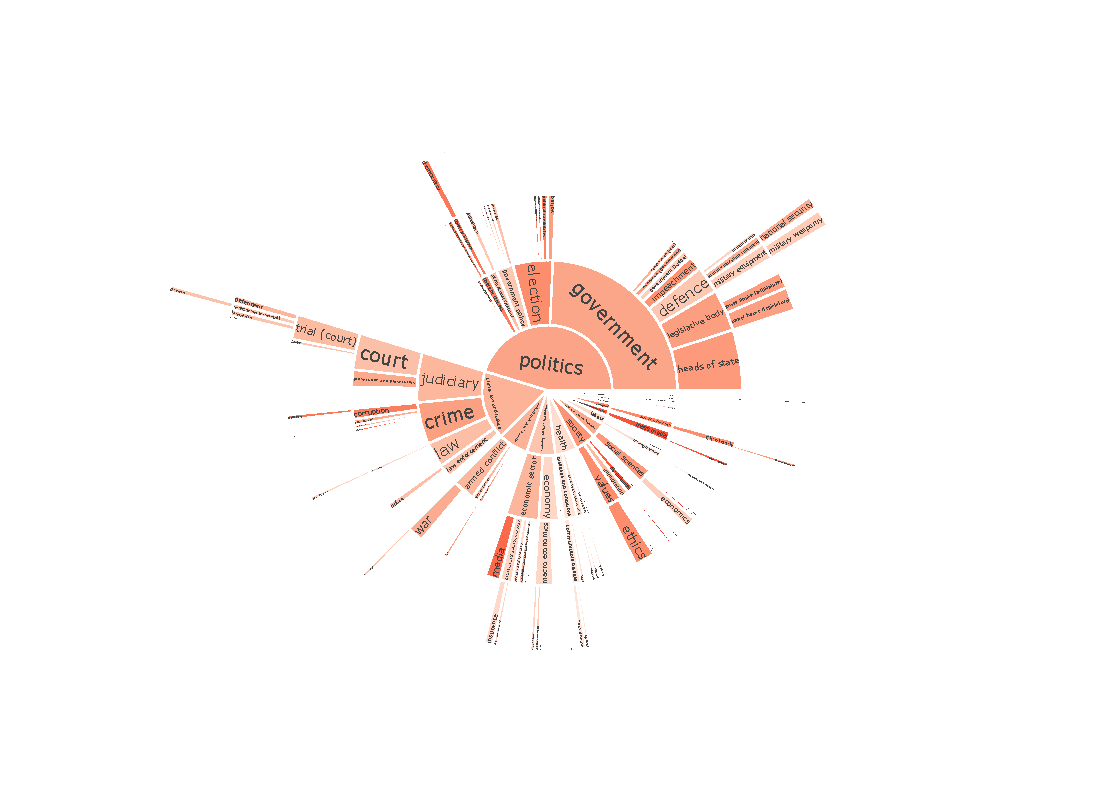
\includegraphics[trim={2.65cm 0cm 0cm 0cm},clip,width=\linewidth]{figures/baly_iptc_weighted_prop_tech_Name_Calling-Labeling.pdf}}
		\caption{Name Calling / Labeling}
            \label{fig:baly_iptc_weighted_prop_tech_Name_Calling-Labeling}
	\end{subfigure}
	
    \caption{Quantity of propaganda techniques across Media Topics}
    \label{fig:baly_iptc_weighted_prop_tech}
\end{figure}

Figure~\ref{fig:baly_iptc_weighted_prop_tech} shows the four major techniques across Media Topics. We suggest to look at the values on the interactive visualisation\footnote{\url{https://martinomensio.github.io/phd-project/figures/baly_iptc_weighted_prop_tech.html}} where it is possible to select which techniques to visualise, hover on the nodes and see the percentage values, and as well to click on the topics and expand on subtopics.

Here we enumerate, for each technique, the topics where they appear the most:
% \todoAW{I wonder whether it would make more sense to show a bar chart (or similar) for each of the techniques?}

\begin{enumerate}
    \item \texttt{Loaded\_Language}: it is the most common technique, as seen in Chapter~\ref{ssec:lp_techniques_propaganda_stats}. Specifically, these topics contain the highest values: \texttt{racism} ($2.4\%$), \texttt{discrimination} ($2.2\%$), \texttt{mass-media }($2.2\%$) and \texttt{corruption} ($1.9\%$). These are topics where the opinions are strong and the media uses strong terms to describe the events.
    \item \texttt{Doubt}: as for \texttt{Loaded\_Language}, the highest quantities are in \texttt{mass-media} ($2.2\%$) and \texttt{corruption} ($1.9\%$). Then we also find \texttt{impeachment} ($1.65\%$), \texttt{national-security} ($1.5\%$) and \texttt{ethics} ($1.4\%$). For these topics, we find that \texttt{Doubt} is especially used to question the reliability of institutions.
    %as questioning the institutions (especially for \texttt{impeachment} and \texttt{national-security}).
    \item \texttt{Flag-waving}: \texttt{racism} ($2.0\%$) and \texttt{discrimination} ($1.7\%$) as in the previous cases, but also notably in \texttt{religion} ($1.3\%$), \texttt{war} ($1.2\%$), \texttt{terrorism} ($1.3\%$) and \texttt{fundamental-rights} ($1.3\%$). These are the topics where the nationalism of flag-waving finds the best environment.
    \item \texttt{Name\_Calling/Labelling}: some topics that emerged also with the previous techniques, such as \texttt{mass-media} ($1.6\%$), \texttt{discrimination} ($1.9\%$), \texttt{media} ($1.4\%$), and \texttt{corruption} ($1.3\%$). But also \texttt{Democracy} ($1.3\%$) that did not emerge with other techniques. \texttt{Name\_Calling} uses resonating and evoking terms that fit with topics related to ethical principles about democracy.
    \item \texttt{Appeal\_to\_fear/Prejudice}: the values are quite low, only showing some small strength in \texttt{armed-conflict} ($0.3\%$), \texttt{military-equipment} ($0.3\%$) and \texttt{communicable-diseases} ($0.3\%$). The distributions for \texttt{diseases} topics is focused on the most recent articles of the dataset (dataset only includes articles until 21 July 2020).
    \item \texttt{Causal\_Oversimplification}: all the values are low, except in the topics \texttt{discrimination} and \texttt{racism} ($0.4\%$). This makes sense with the nature of the topics, and the news articles treating them may report fallacious reasoning containing oversimplifications.
    \item \texttt{Slogans}: all values are low, except in the topics \texttt{civil-unrest} ($0.4\%$), \texttt{police} ($0.2\%$) and \texttt{racism} ($0.2\%$). This makes sense with the protests happened in the time interval included in the dataset. 
\end{enumerate}

These topic-technique associations verify the theoretical aspects of propaganda and show evidence of patterns that we know from the literature.

% \subsection{Terms of propaganda across Media Topics}
% terms of propaganda by topic?



% \subsection{Coarse Topics}
% \todo{REMOVE SUBSECTION: using coarse topics, heatmaps and no finding: "All three political leanings have very similar profiles, with some exceptions"}

% TextRazor has Coarse Topics (up to 5 topics for each article, article-level, e.g. Health/Politics/Law/...) and topics (more fine-grained, around 200 for each article). Each coarseTopic and topic has a weight score which is a value between 0 and 1 representing how prominent is that topic in the article.
% Idea: topic+propaganda techniques
% Which topics are there?
% Which topics co-occur most with propaganda?
% Observe how L/C/R use each propaganda technique in a specific topic



% \subsubsection{Which topics co-occur most with propaganda?}
% This is done at the document level.
% Co-occurrence: heatmap propaganda techniques and topics

% the biggest co-occurrence is between topic violence and technique loaded language.
% BUT it’s only a consequence of Violence and Politics occurring more than other topics in the dataset
% Solution: for each cell divide by the sum of topic quantity. An article can have multiple topics. The values used for the weighting of the matrices are the same for all the rows.

% TODO FIGURE

% (each cell is sum(prop\_quantity*topic\_quantity) / sum(topic\_quantity))
% Each cell represents the average quantity of each propaganda technique for the articles that have been tagged to that topic (considering the topic weight)


% All three political leanings have very similar profiles, with some exceptions

\subsection{\statusgreen Discussion}

Our RQ4.1 for this section was \emph{How does detected propaganda differ across polarising versus neutral topics?}

We have analysed how propaganda changes across Media Topics, which are our selected methodology from Sec~\ref{sec:topic_topic_granularities}.
First, we analysed which topics contain more propaganda overall (Subsection~\ref{ssec:topic_propaganda_tot}), finding a group of topics that are very loaded with propaganda (\texttt{sexism}, \texttt{racism}, \texttt{discrimination}, \texttt{corruption}) and as well topics with very low values (\texttt{economy}, \texttt{health}, \texttt{defence}).
Then we considered the propaganda techniques individually (Subsection~\ref{ssec:topic_propaganda_tech}), and found very specific topic-technique associations.

With this analysis we still do not have a picture of how the political orientation interacts with these loaded areas. Therefore, in the next section, we address RQ4.2, introducing the political leaning in the analysis.



\section{\statusgreen Propaganda across Topics and Leanings}
\label{sec:topic_propaganda_leaning}

In previous Chapter~\ref{chap:political_sides} we observed how propaganda changes across political leanings.
In this chapter, we combine that analysis with the analyses across topics (previous Leaning across Topics, Section~\ref{ssec:topics_topics_leaning}, and Propaganda across Topics~\ref{sec:topic_propaganda}).
In this way, we have an analysis that considers the three variables (Propaganda, Leaning and Topic) all together to discover associations and major differences across Leanings.

This analysis aims at verifying whether propaganda is used by news sources (associated with specific leanings) for certain topics in a very recognisable way to push for a certain idea or a certain narrative.

Our RQ4.2 is: \emph{How does detected propaganda differ across political leaning in polarising and neutral topics?}
While answering this question, we seek multiple objectives:

\begin{enumerate}
    % \item discover associations of topic + leaning that have strong propaganda; --> not easy to show and compare
    % \item discover associations of topic + leaning + techniques that are used frequently together; --> not easy to show and compare
    \item identify topics where propaganda is very different across political leaning considering the \emph{quantity};
    \item identify topics where propaganda is very different across political leaning, considering the \emph{terms} used.
\end{enumerate}

% We tried first to consider the analysis done in Figure~\ref{fig:baly_iptc_weighted_by_leaning} and break it down with respect to the political leaning.
% But to make it easier t
To see and compare the results between leanings, we opted to use the difference of the total quantity of propaganda (Subsection~\ref{ssec:topic_propaganda_leaning_tot_quantity}) and the correlation of the quantities of the techniques across Left and Right (Subsection~\ref{ssec:topic_propaganda_leaning_tot_quantity}) and the correlation of the propaganda terms (Subsection~\ref{ssec:topic_propaganda_leaning_terms}). 



% Experiment 4.3: 
% - topic breakdown: AllSides Topics, IPTC
% - shapes of propaganda/sentiment (leaning)


% Types of shapes (propaganda)
% (look at purple: propaganda)

% Blue is sentiment (+ and -) and purple is propaganda. 
% y axis in the fraction of terms marked as sentiment/propaganda.

% \subsection{\statusred Finding associations of Topic and Leaning with Propaganda}

% As for the first objective, we consider the analysis done in Figure~\ref{fig:baly_iptc_weighted_by_leaning} and we break it down with respect to the political leaning.
% This means that we have the three following 

% - for each leaning, see max propaganda values across topics

% \subsection{\statusred Finding associations of Topic and Leaning with specific Propaganda Techniques}

% - for each leaning, see max propaganda values (by technique) across topics

\subsection{\statusgreen Topics with more Propaganda in Left vs Right}
\label{ssec:topic_propaganda_leaning_tot_quantity}

% - total quantity: max difference
% - techniques: correlation analysis

The first comparison that we do is with the total quantity of propaganda. We want to see in which topics Left is using more propaganda than Right.
The easier way to compare this, is by considering the analysis of Figure~\ref{fig:baly_iptc_weighted_by_leaning} and consider the leaning of the articles. Three separate arrays of values are built (values for each topic are computed separately):
%, one for each political leaning, containing values for each topic:
the first one representing the average propaganda quantity of articles from the Left, the second one from the Center, the third from the Right.
We then subtract the values from the Left with the values from the Right, and we have a score that represents
the relative difference in quantity of propaganda between the Left and the Right, for each topic.


% For the total quantity, it is a single value. So we can only compare if it is greater or smaller. We therefore compute the difference of total propaganda quantity Left - Right.

\begin{figure}[!htbp]
    \centering
    \href{https://martinomensio.github.io/phd-project/figures/baly_iptc_weighted_prop_total_leaning_diff.html}{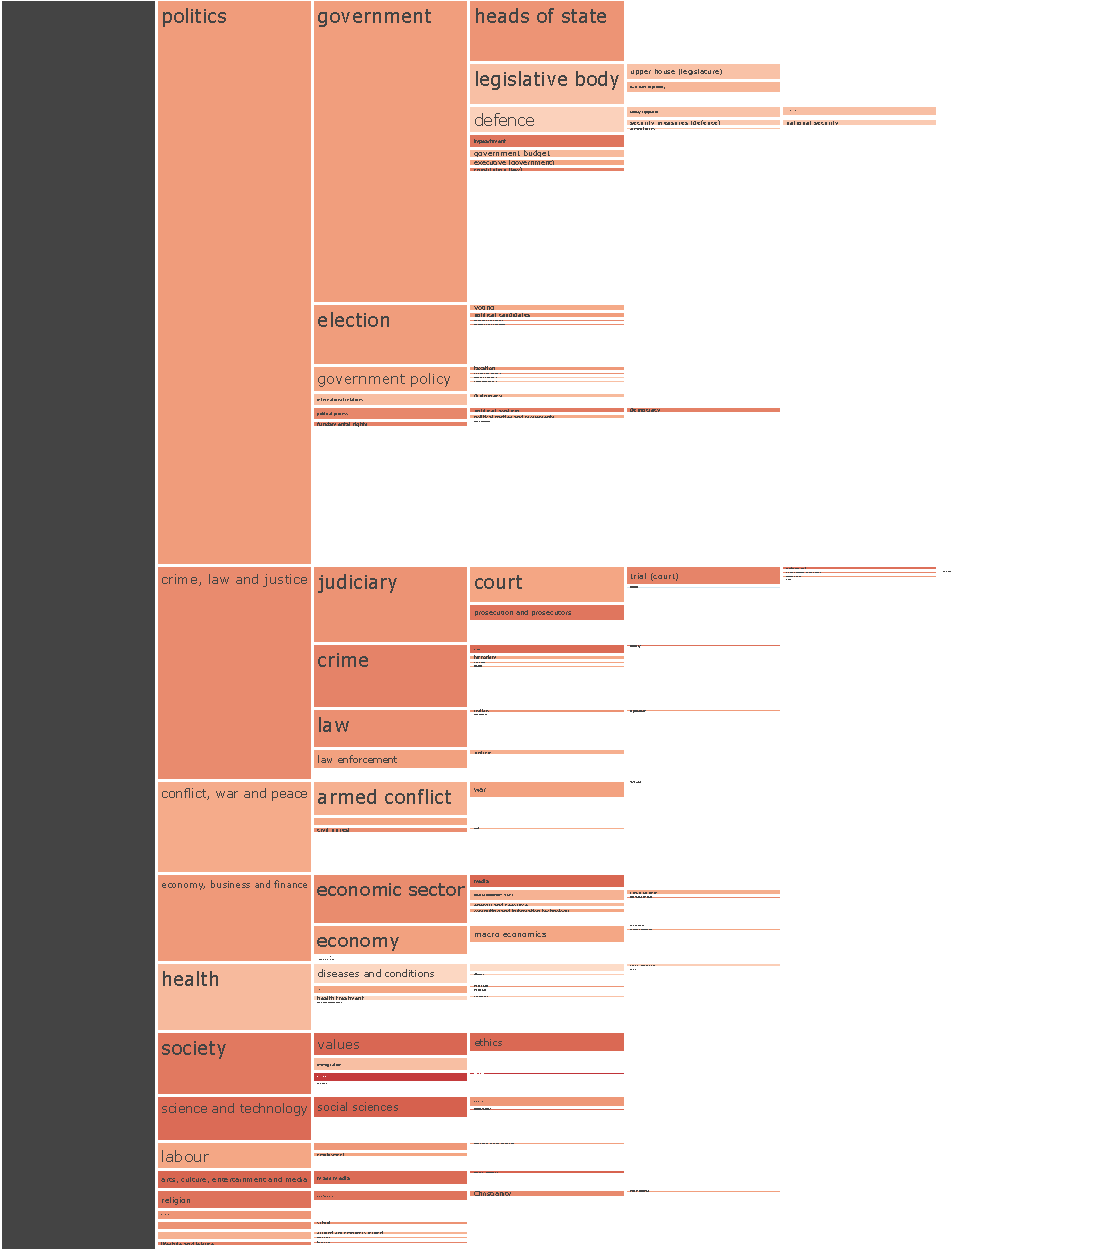
\includegraphics[trim={2.65cm 0cm 0cm 0cm},clip,width=\linewidth]{figures/baly_iptc_weighted_prop_total_leaning_diff.pdf}}
    \caption{Comparison of propaganda quantity across leaning: Left (blue) vs Right (red).}
    \label{fig:baly_iptc_weighted_prop_total_leaning_diff}
\end{figure}

Figure~\ref{fig:baly_iptc_weighted_prop_total_leaning_diff}
% \todoAW{All looks red to me.} 
shows the resulting diagram.\footnote{\url{https://martinomensio.github.io/phd-project/figures/baly_iptc_weighted_prop_total_leaning_diff.html}}
As we can see, the majority of the topics have more Right-leaning propaganda (the figure is almost all red). As we saw in the previous chapters, propaganda is detected more on Right-leaning articles.
This prevalence can be seen especially on some topics: \texttt{ethics} ($1\%$), \texttt{discrimination} ($2\%$), \texttt{media} ($1\%$) and corruption ($1\%$).
Instead, Figure~\ref{fig:baly_iptc_weighted_prop_total_leaning_diff_zoom} shows that when we zoom on specific subtopics, we also see some that have more Left-leaning propaganda:
%that have a prevalence of Left-leaning propaganda:

\begin{figure}[!htbp]
    \centering
	\href{https://martinomensio.github.io/phd-project/figures/baly_iptc_weighted_prop_total_leaning_diff.html}{\begin{subfigure}{0.49\textwidth}
		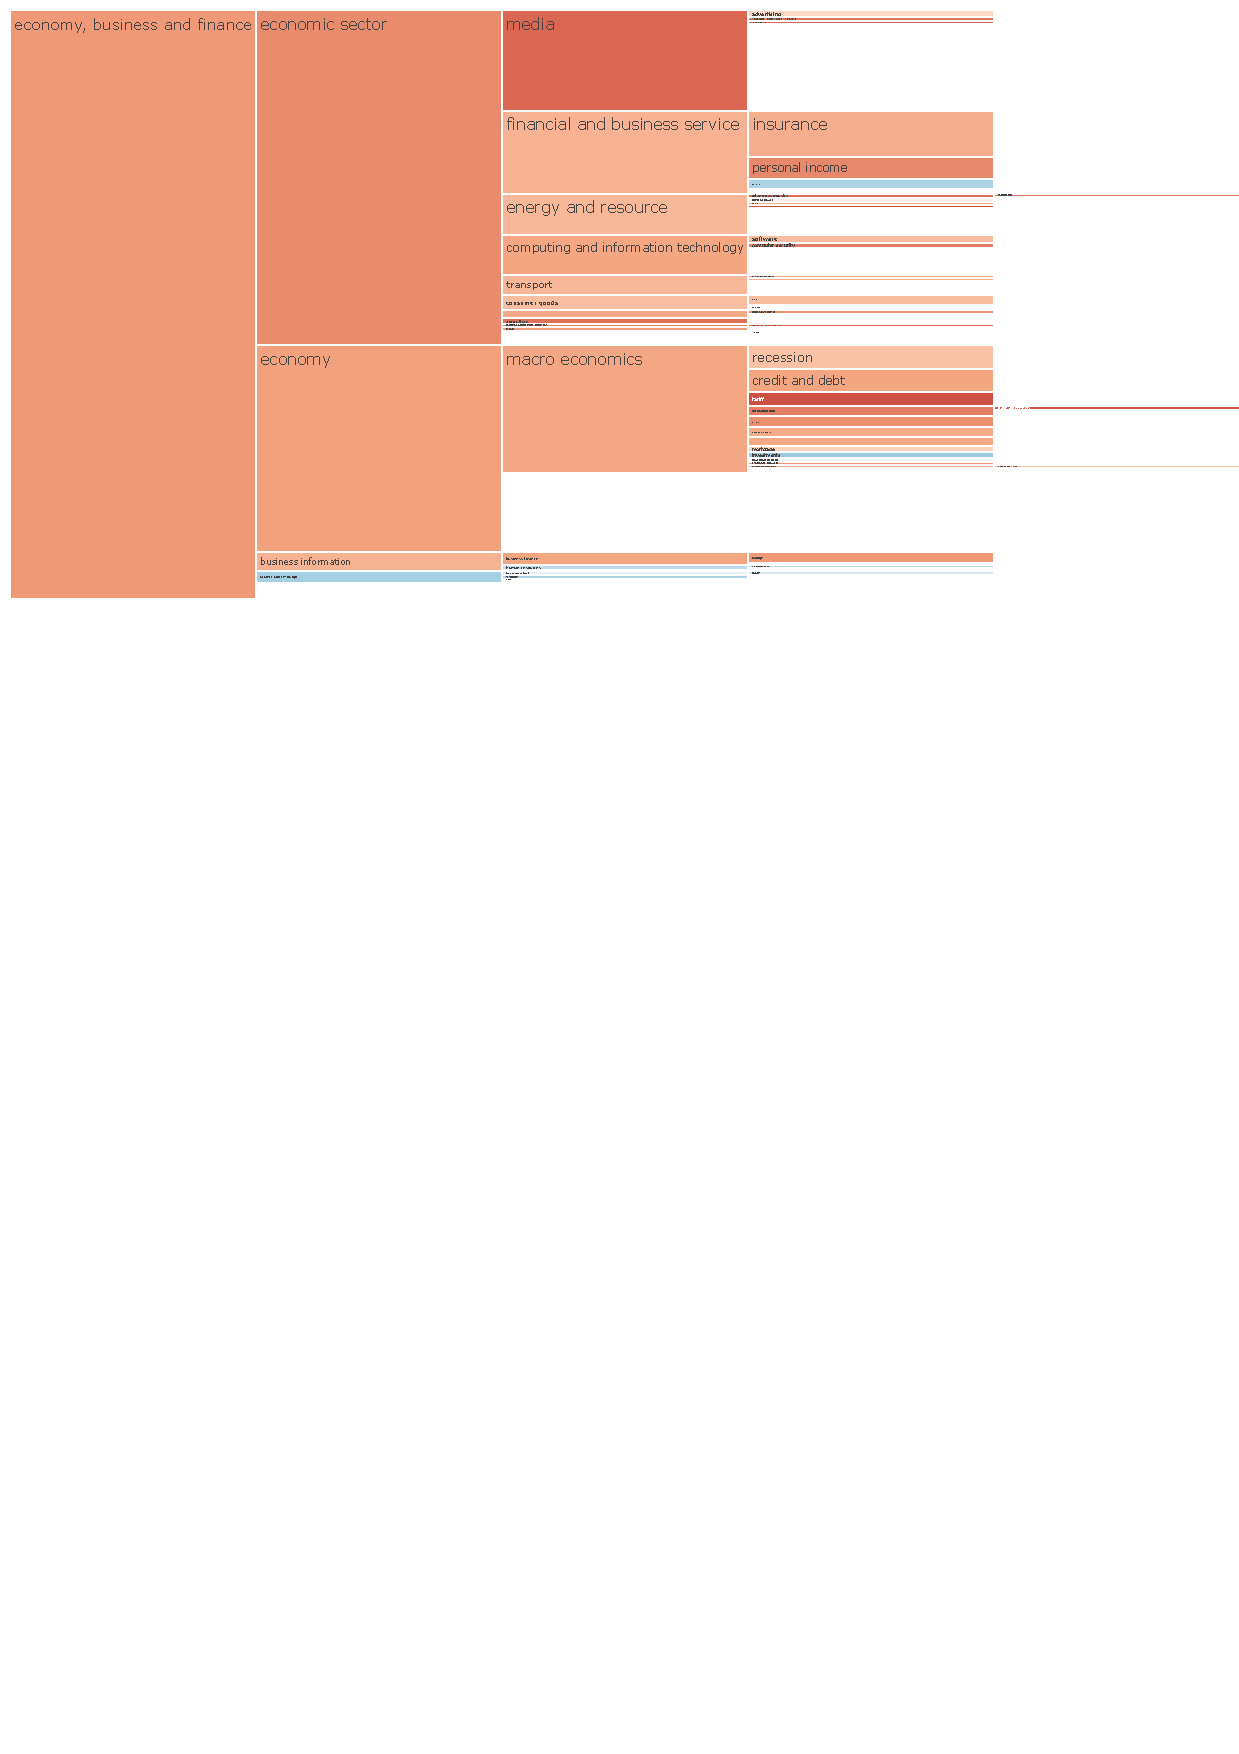
\includegraphics[trim={0.15cm 19.5cm 5cm 0.15cm},clip,width=\linewidth]{figures/baly_iptc_weighted_prop_total_leaning_diff_zoom_economy.pdf}
		\caption{\texttt{economy-business-and-finance}}
            \label{fig:baly_iptc_weighted_prop_total_leaning_diff_zoom_economy}
	\end{subfigure}
	\begin{subfigure}{0.49\textwidth}
		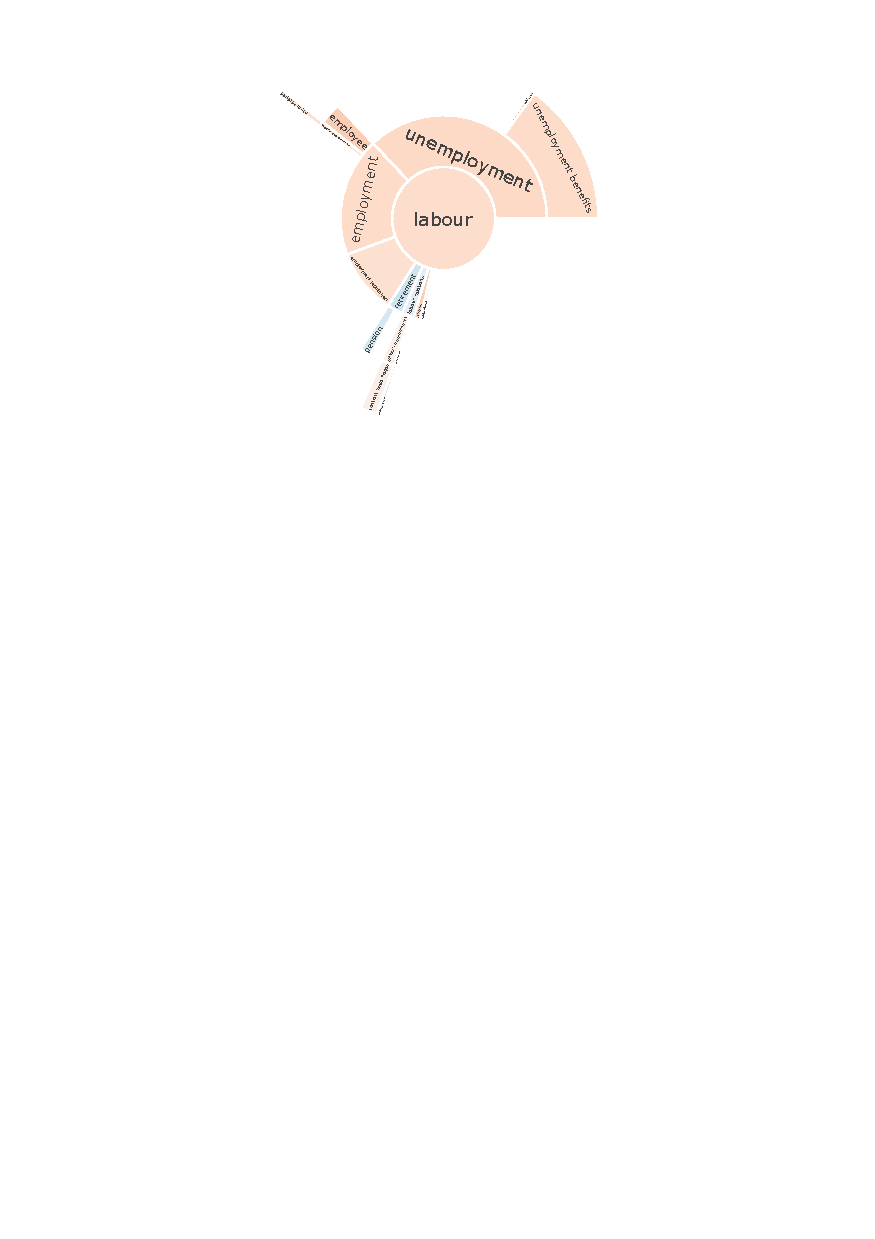
\includegraphics[trim={0.15cm 19.5cm 5cm 0.15cm},clip,width=\linewidth]{figures/baly_iptc_weighted_prop_total_leaning_diff_zoom_labour.pdf}
		\caption{\texttt{labour}}
            \label{fig:baly_iptc_weighted_prop_total_leaning_diff_zoom_labour}
	\end{subfigure}
	\begin{subfigure}{0.49\textwidth}
		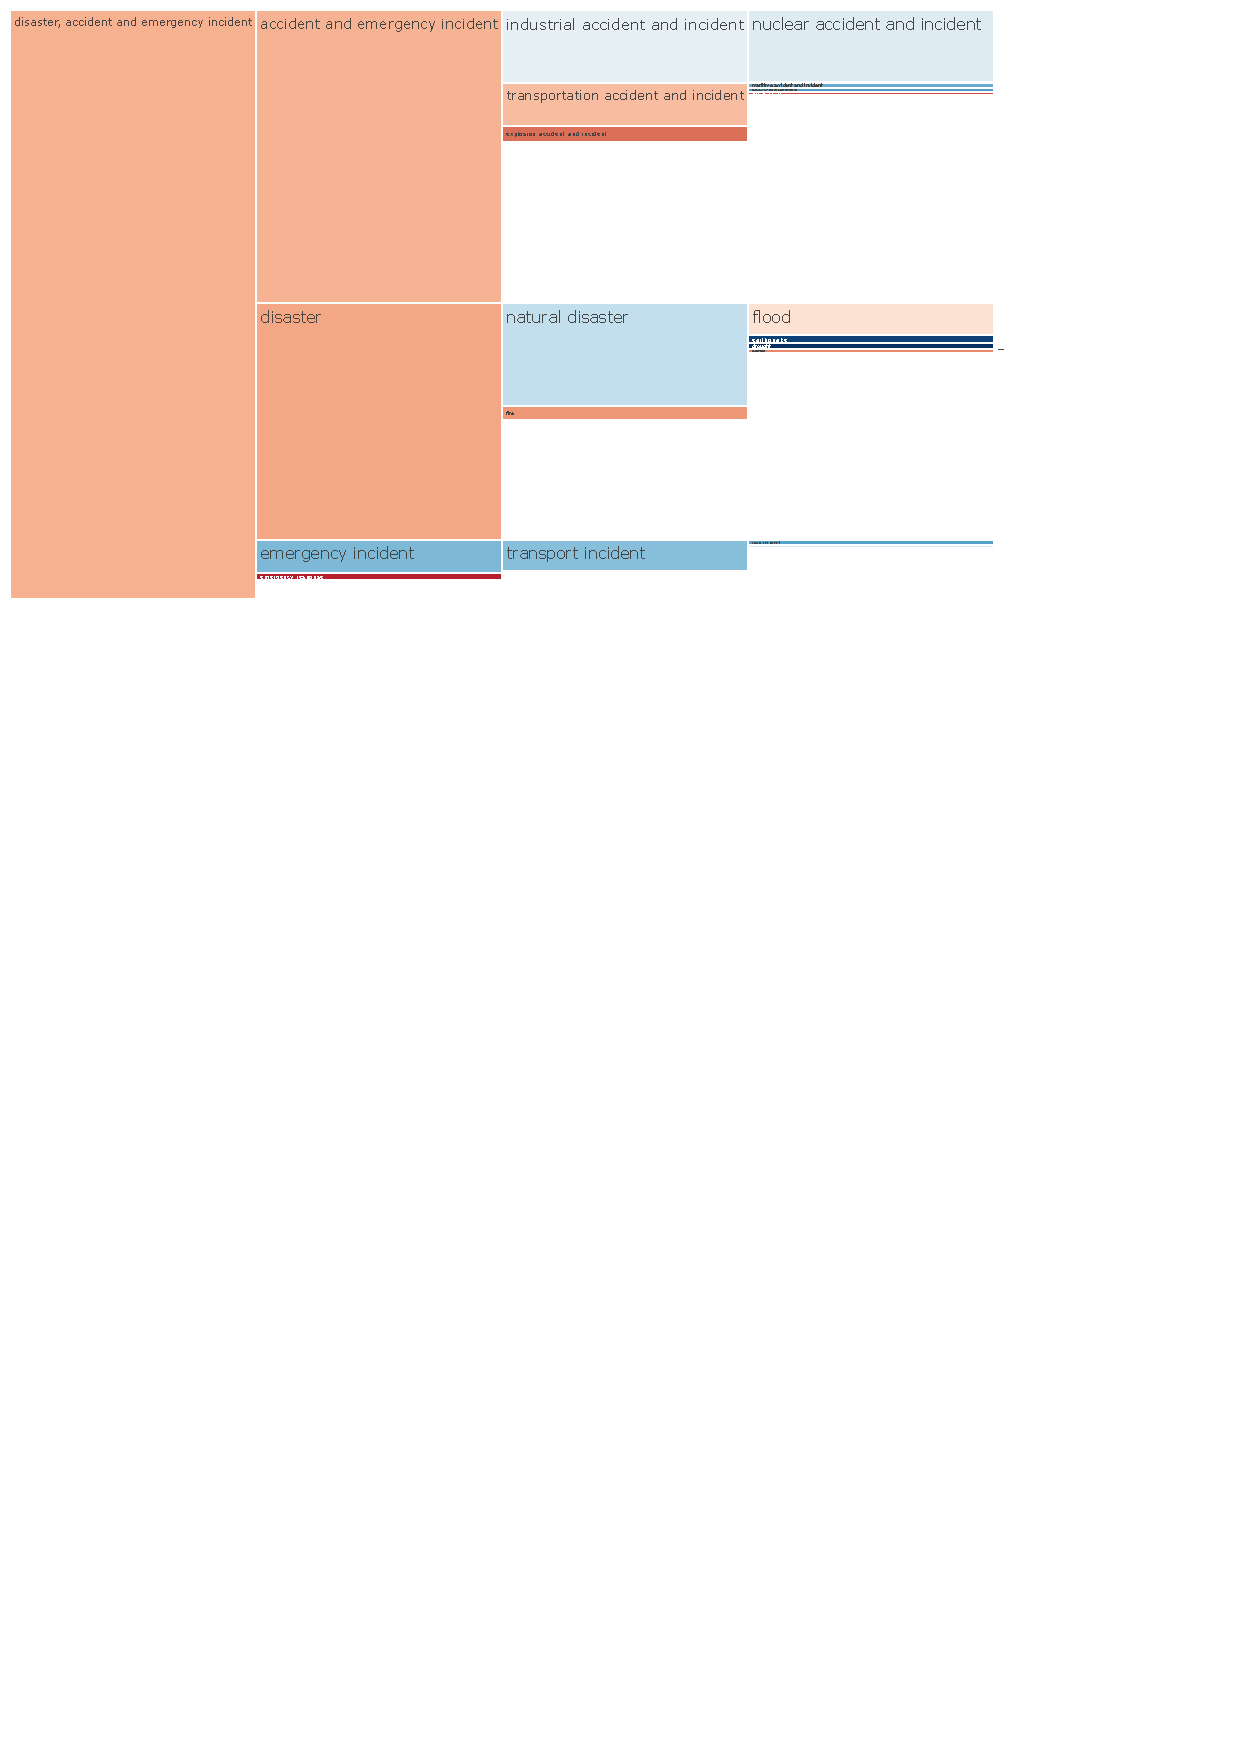
\includegraphics[trim={0.15cm 19.5cm 5cm 0.15cm},clip,width=\linewidth]{figures/baly_iptc_weighted_prop_total_leaning_diff_zoom_disaster.pdf}
		\caption{\texttt{disaster-accident-and-emergency}}
            \label{fig:baly_iptc_weighted_prop_total_leaning_diff_zoom_disaster}
	\end{subfigure}
	\begin{subfigure}{0.49\textwidth}
		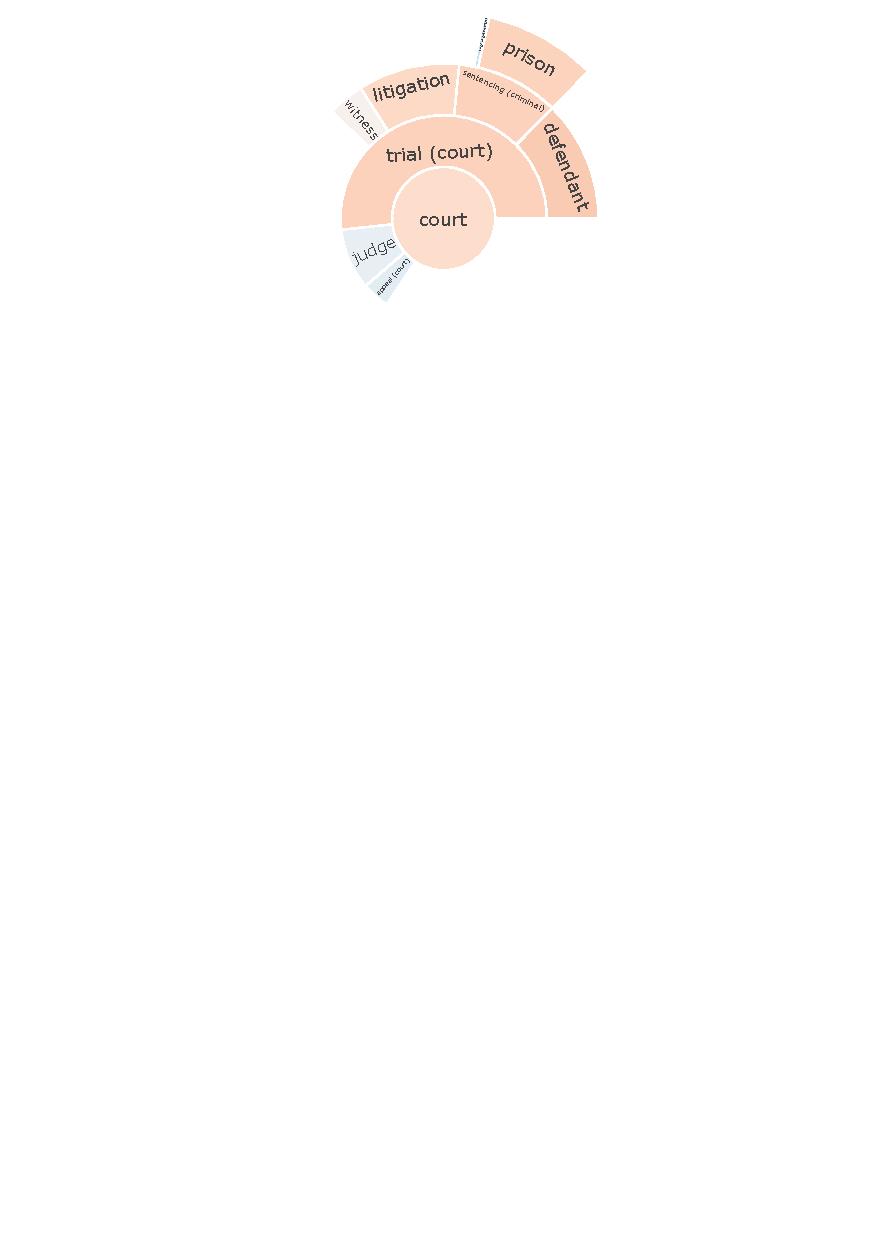
\includegraphics[trim={0.15cm 19.5cm 5cm 0.15cm},clip,width=\linewidth]{figures/baly_iptc_weighted_prop_total_leaning_diff_zoom_court.pdf}
		\caption{\texttt{court}}
            \label{fig:baly_iptc_weighted_prop_total_leaning_diff_zoom_court}
	\end{subfigure}}
	
    \caption{Zoom on specific topics: Left (blue) vs Right (red) propaganda}
    \label{fig:baly_iptc_weighted_prop_total_leaning_diff_zoom}
\end{figure}

\begin{itemize}
    \item \texttt{economy-business-and-finance} (top-level topic): the subtopics that have more Left-leaning propaganda  are \texttt{banking} ($0.4\%$), \texttt{investments} ($0.5\%$), \texttt{market-and-exchange} ($0.5\%$). The rest of the subtopics contain more Right-leaning propaganda.
    \item \texttt{labour} (top-level topic): \texttt{retirement} ($0.8\%$), \texttt{pension} ($0.6\%$) and \texttt{labour} \texttt{strike-dispute} ($0.5\%$). Also here, the rest is mostly Right-leaning propaganda.
    \item \texttt{disaster-accident-and-emergency-incident}: Left-leaning articles contain higher quantity of propaganda on the subtopics of \texttt{drought} ($4.4\%$) and \texttt{earthquake} ($3.5\%$) when compared to the Right. Also the subtopics of \texttt{emergency-incidents} ($0.8\%$), \texttt{railway-incidents} ($1.3\%$) and \texttt{maritime-incidents} ($1.0\%$) get more propaganda in the Left, while \texttt{road-accidents} get more in the Right ($1.7\%$).
    \item \texttt{court} (\texttt{crime-law-and-justice} $\rightarrow$ \texttt{judiciary}): here most of the propaganda is from the Right, except from \texttt{capital-punishment} ($1.0\%$).
\end{itemize}

From this analysis, we can see that even though the quantity of propaganda is substantially higher in the Right, we can be able to identify some topics where instead the Left is using quite strong persuasion means.
The identified topics with more Left-leaning propaganda are topics where the Left has the strongest opinions. For example, in regards to \texttt{capital-punishment} the Left has a strong opposition, while the Right might be less strong with language when covering this topic because it generally accepts more this practice.
Or if we consider the types of accidents, it is meaningful that the Right is using stronger language when talking about \texttt{road-accidents}, while the Left is more on \texttt{railway} and \texttt{maritime}. Furthermore, the Left has a stronger language when covering natural disasters (\texttt{earthquake} and \texttt{drought}), as they are usually related to bad environmental practices, a theme for which the Left usually shows its opposition.

The language contains more propaganda and is stronger when the writer either considers the topic more important, or is criticising the status quo~\citep{rose1992political}.
% We confirm this with our analysis.  


\subsection{\statusgreen Correlation of Propaganda Quantities between Leanings across Topics}
\label{ssec:topic_propaganda_leaning_tech_quantities}

% Propaganda techniques: difference
% - techniques: correlation analysis


% Propaganda techniques: correlation analysis (how different)

For the next step, we take into consideration the different techniques. We want to study how the usage of propaganda techniques is correlated across leanings on several topics.
%
First, by studying the correlation of the \emph{quantities} of each technique. Then, in the next subsection, we will observe the correlation of the TF-IDF features (\emph{terms}).

The idea is to take for each topic and leaning the 18 values that represent the average quantity of the propaganda techniques for articles of that leaning. With these, we compute the correlation of the values of the Left against the values of the Right.
%
As correlation metric, we choose to use Pearson because it works with normal and half-normal distributions~\cite{pearson1931analysis}.
% The distribution of the propaganda scores is half-normal therefore Pearson is the best metric.\todoAW{Needs more explanation}
% \todoAW{numbers for the half-normal distribution, more details}

\begin{figure}[!htbp]
    \centering
    \href{https://martinomensio.github.io/phd-project/figures/baly_iptc_weighted_prop_leaning_corr.html}{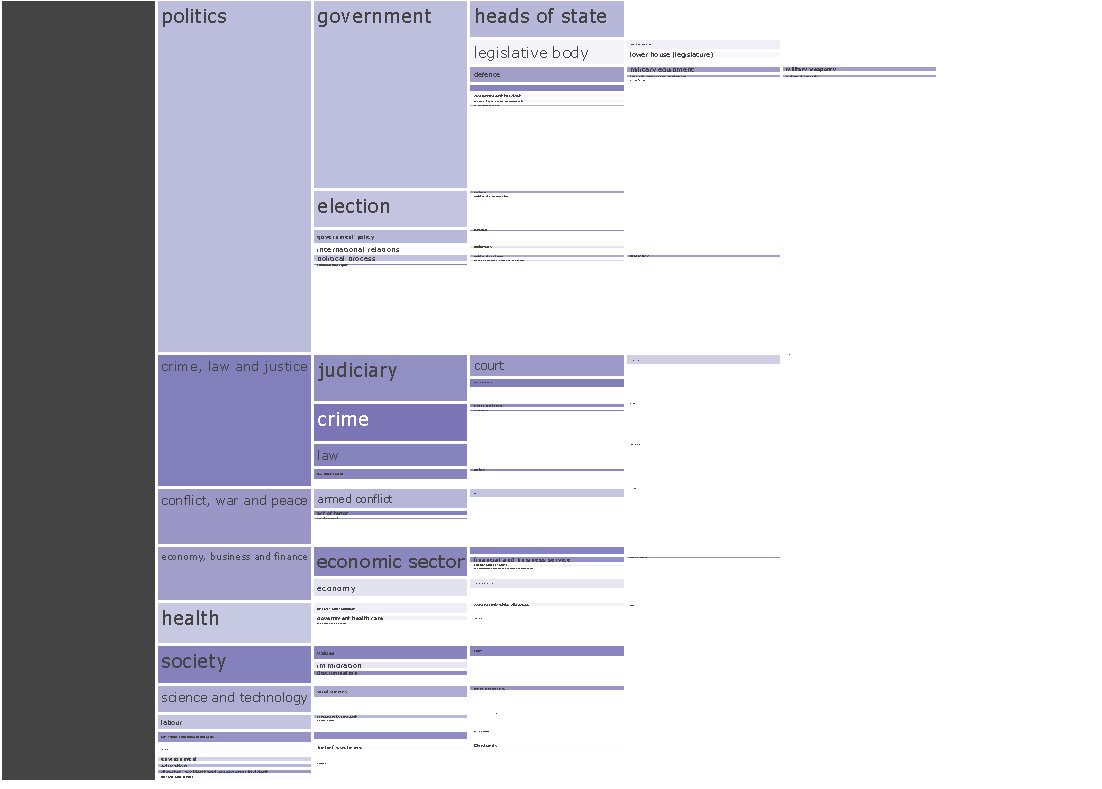
\includegraphics[trim={2.65cm 0cm 0cm 0cm},clip,width=\linewidth]{figures/baly_iptc_weighted_prop_leaning_corr.pdf}}
    \caption{Correlation of quantities of propaganda techniques between Left and Right: light purple (low correlation) to dark purple (high correlation).}
    \label{fig:baly_iptc_weighted_prop_leaning_corr}
\end{figure}

Figure~\ref{fig:baly_iptc_weighted_prop_leaning_corr} shows the resulting diagram.\footnote{\url{https://martinomensio.github.io/phd-project/figures/baly_iptc_weighted_prop_leaning_corr.html}}
We show on a scale of purples the correlation values between the left and the right values.
The correlation values are very high for all the topics ($96\% - 100\%$), therefore we select this range in the colour scales, to see the differences more easily.
Even zooming on specific subtopics, the correlation rarely falls under $90\%$: under \texttt{economic-sector}, \texttt{chemicals} ($87.2\%$) and \texttt{air-transport} ($84.0\%$); under \texttt{macro-economics}, \texttt{exports} ($50.9\%$). 
These subtopics, however, are quite small and have a count lower than $50$ (keep in mind that belonging to a topic is a floating number). As a consequence of this, the results are no longer significant when restricting to such a small number of articles.

Therefore, even though the total quantity of propaganda may be different across the leaning (as found in the previous subsection), we find that that the correlation remains very high.
%also in those topics that showed the difference in the total.\todoHA{??}
This means that what changes is the total quantity of propaganda, but not the relative proportions of the techniques used.

\subsection{\statusgreen Term Correlation between Leanings across Topics}
\label{ssec:topic_propaganda_leaning_terms}

The last step of this correlation analysis is to see whether the \emph{terms} of propaganda are correlated between them.
% We have just seen that the correlation is very high when considering only the quantities of each technique

To analyse this, we take the term features already computed in Chapter~\ref{chap:political_sides} and~\ref{chap:linguistic_persuasion}.
This feature set is made of TF-IDF computed on the whole dataset with a feature size of 2000.
% \todoHA{Any rationale of why 2k?}
% across the  together.
We choose this number of features to be able to capture enough terms. Over-sizing this value does not have negative effects beyond making the computation longer.

In order to compute the specific TF-IDF feature for each topic and leaning, we iterate over the dataset and we accumulate the TF-IDF of single articles into buckets that are identified by leaning and media topic.
Alongside, we also accumulate the weights of articles belonging to each bucket (leaning is integer, while topic score is a floating number), as in the previous subsections, so that we can compute the average TF-IDF vector for each topic and leaning.
We then take the vectors from the Left and the Right, and we compute the Pearson's correlation as in the previous case.

\begin{figure}[!htbp]
    \centering
    \href{https://martinomensio.github.io/phd-project/figures/baly_iptc_weighted_prop_leaning_corr_tfidf.html}{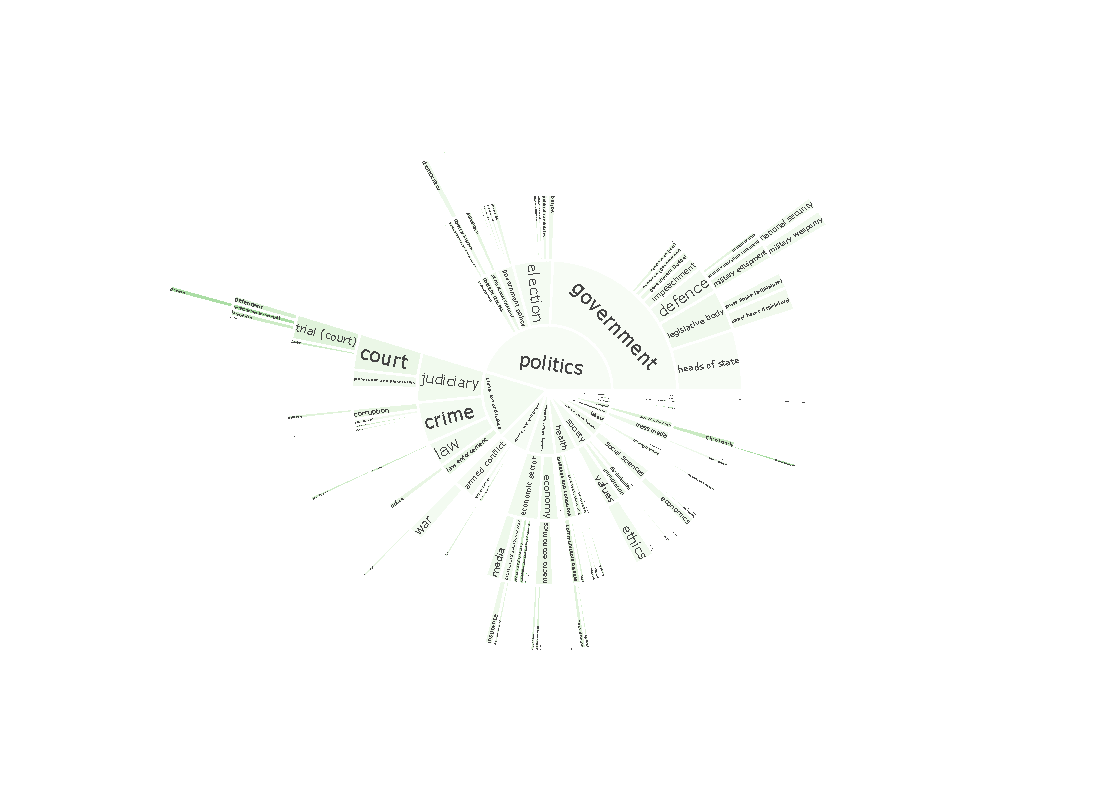
\includegraphics[trim={2.65cm 0cm 0cm 0cm},clip,width=\linewidth]{figures/baly_iptc_weighted_prop_leaning_corr_tfidf.pdf}}
    \caption{Correlation of propaganda terms (TF-IDF features) between Left and Right: light purple (low correlation) to dark purple (high correlation)}
    \label{fig:baly_iptc_weighted_prop_leaning_corr_tfidf}
\end{figure}

Figure~\ref{fig:baly_iptc_weighted_prop_leaning_corr_tfidf} shows the resulting diagram,\footnote{\url{https://martinomensio.github.io/phd-project/figures/baly_iptc_weighted_prop_leaning_corr_tfidf.html}}
%where this time we did not adjust the colour range, because the values of correlation vary from $5\%$ to $98\%$.
where we can see the values of correlation considering the TF-IDF features.
We can see that, with respect to the previous Figure~\ref{fig:baly_iptc_weighted_prop_leaning_corr}, we have some topics where the correlation values are lower than 90\%: subtopics of \texttt{court}, for example, have values as low as $62\%$, or \texttt{fundamental-rights} even reach $5\%$.


% \begin{figure}[!htbp]
%     \centering
% 	\begin{subfigure}{0.45\textwidth}
%             \centering
% 		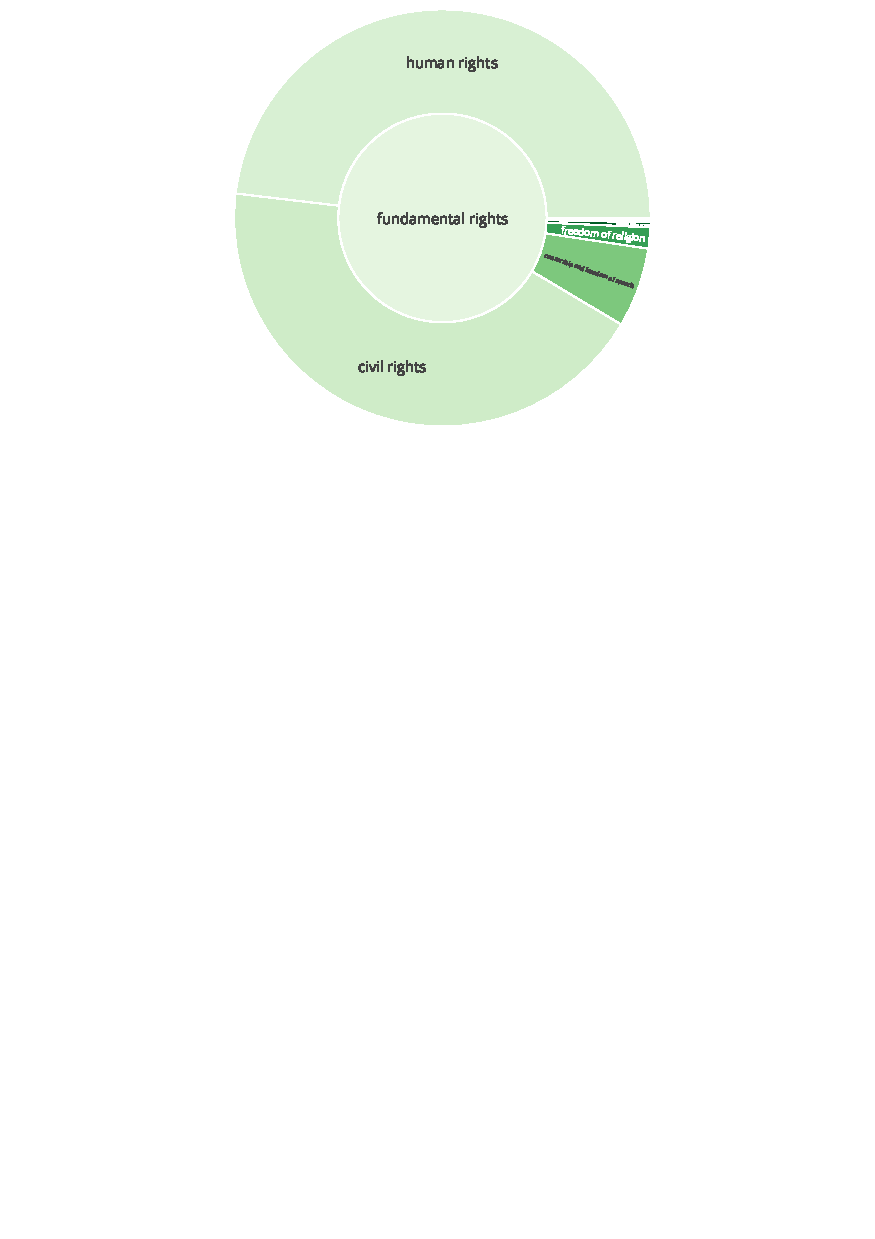
\includegraphics[trim={0 0 0 0},clip,width=0.8\linewidth]{figures/baly_iptc_weighted_prop_leaning_corr_tfidf_zoom_fundamental_rights.pdf}
% 		\caption{Fundamental Rights}
%             \label{fig:baly_iptc_weighted_prop_leaning_corr_tfidf_zoom_fundamental_rights}
% 	\end{subfigure}
% 	\begin{subfigure}{0.45\textwidth}
% 		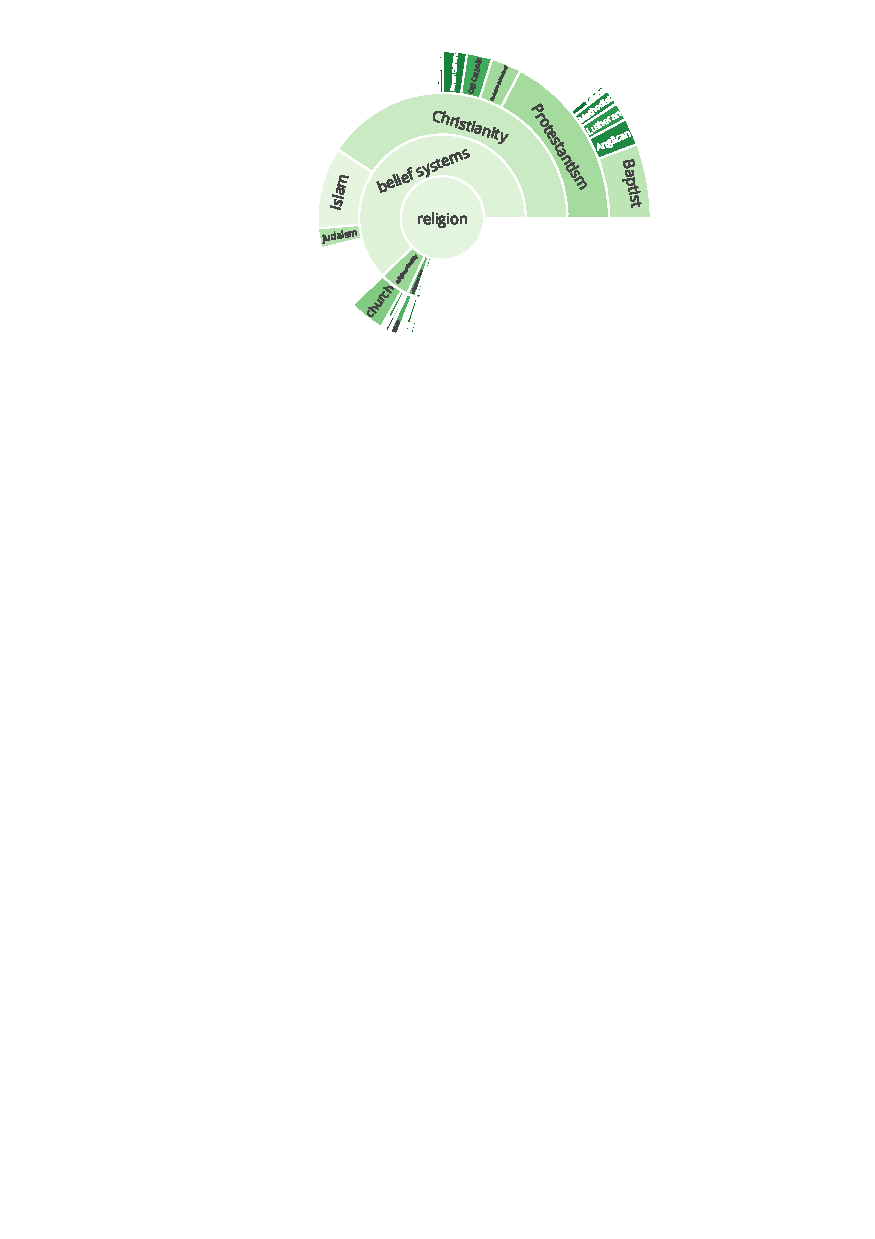
\includegraphics[trim={0 0 0 0},clip,width=\linewidth]{figures/baly_iptc_weighted_prop_leaning_corr_tfidf_zoom_religion.pdf}
% 		\caption{Religion}
%             \label{fig:baly_iptc_weighted_prop_leaning_corr_tfidf_zoom_religion}
% 	\end{subfigure}
% 	\begin{subfigure}{0.45\textwidth}
% 		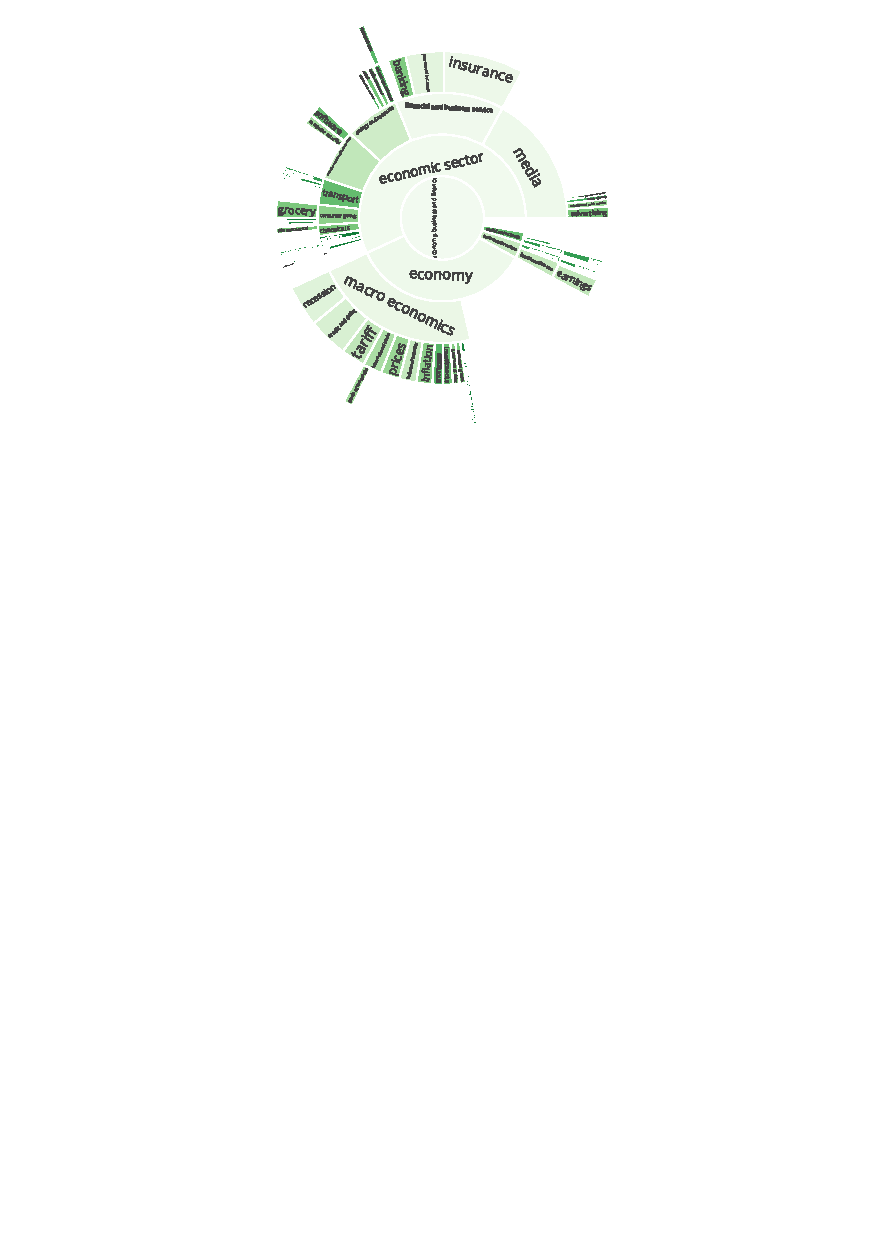
\includegraphics[trim={0 0 0 0},clip,width=\linewidth]{figures/baly_iptc_weighted_prop_leaning_corr_tfidf_zoom_economy.pdf}
% 		\caption{Economy}
%             \label{fig:baly_iptc_weighted_prop_leaning_corr_tfidf_zoom_economy}
% 	\end{subfigure}
% 	\begin{subfigure}{0.45\textwidth}
% 		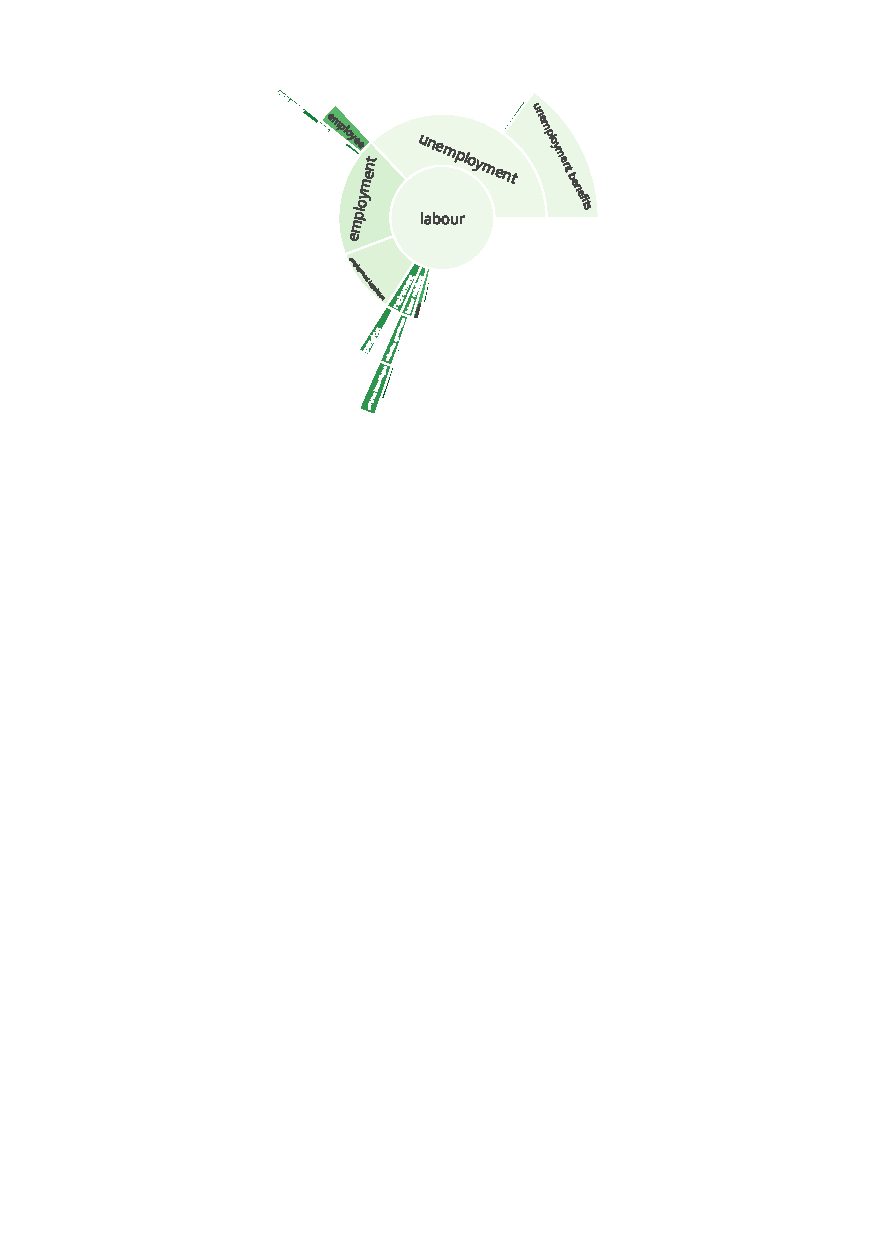
\includegraphics[trim={0 0 0 0},clip,width=\linewidth]{figures/baly_iptc_weighted_prop_leaning_corr_tfidf_zoom_labour.pdf}
% 		\caption{Labour}
%             \label{fig:baly_iptc_weighted_prop_leaning_corr_tfidf_zoom_labour}
% 	\end{subfigure}
% 	\begin{subfigure}{0.45\textwidth}
%             \centering
% 		
\includegraphics[trim={0 0 0 0},clip,width=0.8\linewidth]{figures/baly_iptc_weighted_prop_leaning_corr_tfidf_zoom_disaster.pdf}
% 		\caption{Disaster}
%             \label{fig:baly_iptc_weighted_prop_leaning_corr_tfidf_zoom_disaster}
% 	\end{subfigure}
% 	\begin{subfigure}{0.45\textwidth}
%             \centering
% 		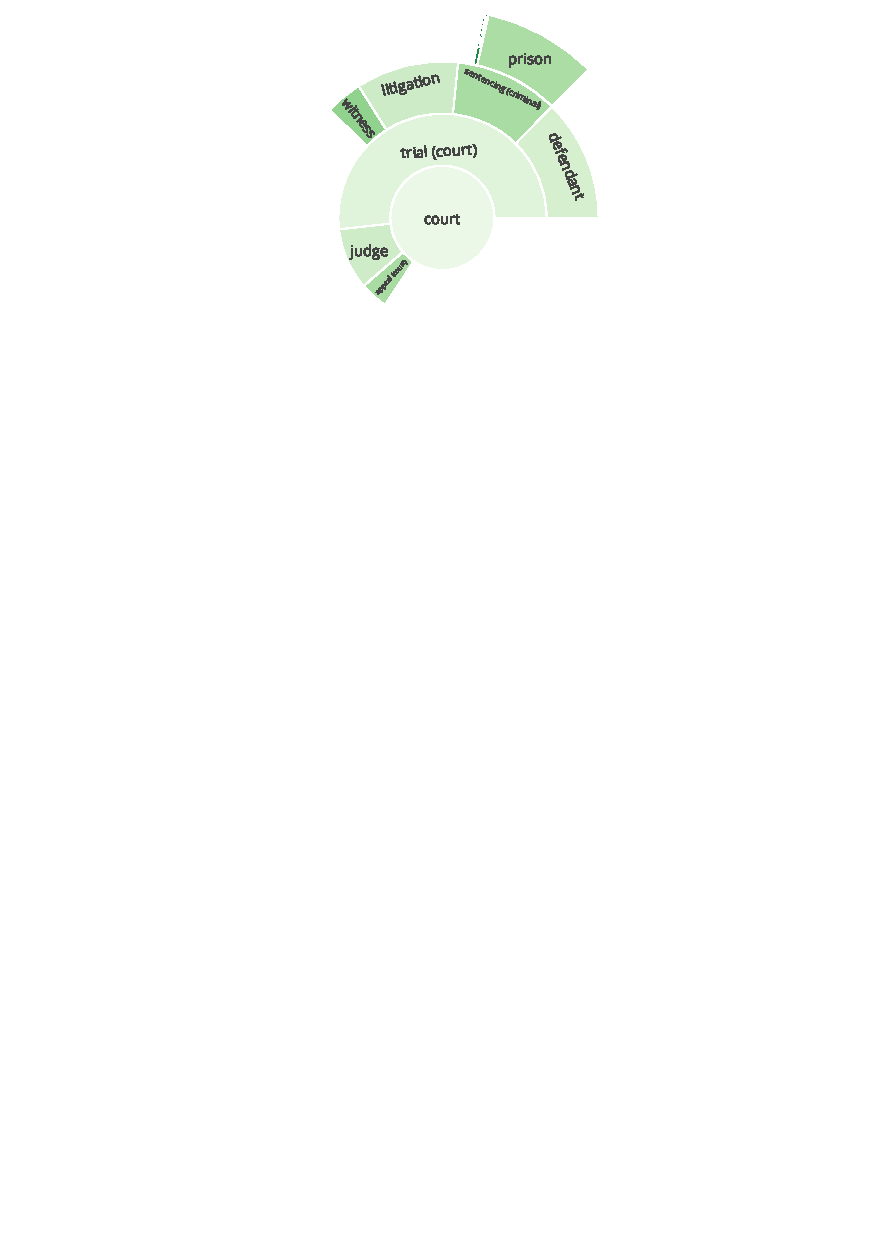
\includegraphics[trim={0 0 0 0},clip,width=0.8\linewidth]{figures/baly_iptc_weighted_prop_leaning_corr_tfidf_zoom_court.pdf}
% 		\caption{Court}
%             \label{fig:baly_iptc_weighted_prop_leaning_corr_tfidf_zoom_court}
% 	\end{subfigure}
	
%     \caption{Zoom on specific topics: correlation of propaganda terms between Left and Right}
%     \label{fig:baly_iptc_weighted_prop_leaning_corr_tfidf_zoom}
% \end{figure}
% \todo{Figure\ref{fig:baly_iptc_weighted_prop_leaning_corr_tfidf_zoom} change colour scale, RE-ZOOM and capture}



We zoom into some of the topics that present low values of correlation to get a clearer view. In these topics, correlation is low, which means that Left and Right are using significantly different propaganda terms.
% Figure~\ref{fig:baly_iptc_weighted_prop_leaning_corr_tfidf_zoom} shows the most important ones.
The lowest values are found in the following topics:

\begin{enumerate}
    \item \texttt{fundamental-rights} (subtopic of \texttt{politics}): on the whole topic, the average correlation is $83.6\%$. The topics where the words differ the most are \texttt{freedom-of-the-press} ($5.5\%$ but very small with a sum of topic weights of 4.16 articles, therefore not significant), \texttt{freedom-of-religion} ($30.3\%$), \texttt{censorship-and-freedom-of-speech} ($49.6\%$). These subtopics were not emerging in our previous analysis, therefore the quantities of propaganda across leaning are quite similar (Subsection~\ref{ssec:topic_propaganda_leaning_tot_quantity}). Instead, considering the propaganda terms used, they differ quite significantly.
    \item \texttt{religion} (top-level topic): we can see here how political leanings use different terminology when talking about many religions. Overall, the correlation for \texttt{religion} is $83.5\%$. \texttt{islam} gets a high correlation ($83.6\%$), while the different branches of \texttt{christianity} ($72.6\%$) are showing less correlation: \texttt{roman-catholic} ($19.1\%$), \texttt{anglican} ($21.6\%$), \texttt{lutheran} ($27.2\%$) are just some examples. This is an interesting finding: when articles are talking about religions through propaganda, we can see that for religions that have been historically more present in the US (main location of the news sources in the \texttt{baly} dataset) we have lower correlation. In other words, for these religions, the debate is more internal and the terms used are more different. Instead, for religions that are generally covered in the news as ``external", the terms used in propaganda are more similar between political leanings.
    \item \texttt{economy-business-and-finance} (top-level topic): these subtopics were already highlighted in Figure~\ref{fig:baly_iptc_weighted_prop_total_leaning_diff_zoom_economy} where we have shown more Left-leaning propaganda in \texttt{banking}, \texttt{investments}, \texttt{market-and-exchange}. Instead here, considering the terms, we can see how the most different topics are specific economic sectors and some macroeconomics categories. For the sectors, the most different are: \texttt{agriculture} ($17.0\%$), \texttt{oil-and-gas-industry} ($40\%$), \texttt{transport} ($43.3\%$). For the macroeconomics: \texttt{economic-indicator} ($19.7\%$), \texttt{mortgage} ($40.0\%$), \texttt{inflation} ($53.6\%$), \texttt{prices} ($57.1\%$). These are mostly topics that have more propaganda on the Right.
    \item \texttt{labour} (top-level topic): this topic was highlighted previously in Figure~\ref{fig:baly_iptc_weighted_prop_total_leaning_diff_zoom_economy}. In this case, the subtopics with lower correlation are the ones that have more propaganda on the Left:  \texttt{retirement} ($26.1\%$), \texttt{pension} ($24.8\%$) and \texttt{labour-strike}/\texttt{dispute} ($7\%$).
    \item \texttt{disaster-accident-and-emergency-incident}: subtopics of \texttt{drought} ($14.8\%$) and \texttt{earthquake} ($23.9\%$). Also the subtopics of \texttt{emergency-incidents} ($0.8\%$), \texttt{railway-incidents} ($31.5\%$) and \texttt{maritime-incidents} ($16.3\%$) \texttt{road-accidents} in the Right ($10.4\%$). In these cases, the unbalance of propaganda was also high.
    \item \texttt{court} (\texttt{crime-law-and-justice} $\rightarrow$ \texttt{judiciary}): here the subtopic with lowest correlation is \texttt{capital-punishment} ($22.2\%$).
\end{enumerate}

\subsection{\statusgreen Discussion}

From these results, we can see that the terms used for propaganda are quite different in specific topics, demonstrated by low correlation values on the TF-IDF features.
In some cases, the low correlation happens in topics where there exists more Left or Right propaganda across the articles (\texttt{economy}, \texttt{labour}, \texttt{disasters}, \texttt{court}). In some other cases instead, propaganda appears uniformly across the spectrum (\texttt{fundamental-rights} and \texttt{religion}) but when we consider the terms we have significant differences (low correlation). Therefore, both the analyses of quantity and terms are necessary.


% \subsection{Custom Topics (AllSides)}
% \todo{REMOVE this subsection. Just check if the main finding is also found with IPTC: Right using Doubt in Science, Center using Appeal to Authority when talking about DEA}

% How do they overlap with the propaganda techniques?

% Every article is tagged with a topic (AllSides) and with the propaganda techniques (from the tool).
% We want to see which topics occur with specific propaganda techniques.
% For this reason, we build 3 heatmaps (one for each political leaning) with the propaganda techniques on the x-axis and the topics on the y-axis. The value of the cell represents the average quantity of the propaganda technique for that specific topic.
% We want to see differences between the Left/Center/Right heatmaps.

% TODO FIGURE: HEATMAP? OR WHAT?

% Differences:
% The Right is using Doubt when talking about “science” far more than the other two political leanings (1.2\% Left - 13 articles, 0.9\% Center - 8 articles, 5.2\% Right - 4 articles). Does this mean that the Right is more sceptical about science? Let’s look at the data (4 articles from the Right with the topic “science”):
% https://spectator.org/science-know-it-alls-on-the-march/
% http://www.washingtontimes.com/news/2017/apr/22/march-political-science-earth-day-rally-doubles-la/ 
% http://www.nationalreview.com/article/447048/bill-nye-science-guy-march-science-left-politics-religion
% https://www.foxnews.com/science/we-could-go-to-venus-with-todays-technology-scientists-say 
% The first 3 articles cover the 25 April 2017 march for science, which was labelled by some sources on the Right as “the leftist [...] new religion” (nationalreview article)
% 3 articles compared here: https://www.allsides.com/story/earth-day-march-science 

% The Center is using Appeal to Authority when talking about “dea” far more than the other two leanings (0\% Left - 3 articles, 1.8\% Center - 1 article, 0\% Right - 1 article). Does the Center appeal more to authority because it is more “moderate” than Left and Right?
% Other cases can be discovered and the classifier can use them (topic+propaganda technique quantity/terms) to recognise political leaning

% \subsubsection{Correlation Left vs Right IPTC}
% Exploratory way: observe the correlation between features of the left and features of the right. If correlation is high, it means that the differences are small. Instead if the correlation is low, it means that there exist differences between left and right.


% Correlation between L/R of Propaganda quantities (18 values for each article) across topics
% The hope is to see that in some subtopics the correlation is low, meaning that the propaganda quantities differ significantly between Left and Right for the subtopic.
% On the full dataset, this propaganda feature was not very useful, so let’s see what happens in all the subtopics.

% TODO figure sunburst spearmans and pearsons

% Scale: blue=correlation high, red=correlation low, grey=not computable (all 0)

% This is clearly a negative result. This means that the propaganda quantities are not useful at all. Let’s check what happens with other features:


% \subsection{Identifying Media Topics with propaganda differences???}

% Objective: using Media Topics taxonomy, find the correct level of narrow that shows differences in how propaganda is used but at the same time not to narrow to still have enough articles.

% Differences (quantities of propaganda techniques across leanings), but with enough support. For the sorting it would be nice to have a formula like: 
% combined\_score = support(topic) * discrepancy
% Or just sort by higher discrepancy, with threshold on support(topic)

% Discrepancy computed as correlation?
% Distribution of propaganda quantities from L and distribution from R
% Option 1: links from AllSides to group the articles in triples
% Option 2: average in topic ← selected as doesn’t need info that articles A and B are on the same story. Correlation between quantities of each technique in L vs R

% \subsection{Testing on coarseTopic}
% Correlation of propaganda techniques quantities between L and R, for each coarseTopic. This is to prove/quantify that coarse topics don’t have much difference in propaganda across political leaning

% TODO FIGURE

% Coarse Topics that have no high correlation:
% Mathematics: pearson=-0.0005, spearman=0.60 (GOOD), support is very small [8. 5. 1.] (BAD)
% Language: pearson=0.86, spearman=0.93. Support is [ 83.  48. 109.] articles

% Pearson vs Spearman: pearson assumes normal distribution, while Spearman no.
% Verifying distribution:

% Histogram of quantity of Loaded Language (most prominent technique) of Left (blue), Center (pink) and Right (red) in all the articles. It looks like a normal distribution, truncated at the 0. Y-axis=percentage (TOO: should verify mathematically how close to normal distribution)

% \subsection{Fine-Grained Topics}
% \todo{REMOVE SUBSECTION: using fine-grained topics but no real result}

% Compute for each topic and each leaning, the co-occurrence with each propaganda technique. Then compute the differences (OK with 2 categories, how to do with 3 categories? Variance? But leaning is on a continuum scale), and sort by difference descending → obtain topics with more differences in propaganda quantities
% Variance: each observation is the average quantity of propaganda in specific leaning+topic, computed across leaning


% :TODO
% Then filter and keep only topics with minimum support (to be defined)

% How to compare / visualise differences between L/C/R across topics?
% Before: heatmaps
% Good only for viewing things from the outside, not too fine-grained

% What about finding differences by ranking with a function that expresses how much difference is there?
% We want topics with high support and have big differences between leaning with respect to a feature (e.g. quantity of a certain technique, term frequencies).

% combined\_score = support(topic) * discrepancy

% Categorical data comparison?

% \subsection{Derived from Entity Types}
% \todo{remove}

% entity propaganda feature computation
% For each entity, compute the total/average propaganda techniques that co-occur in the same sentence by each political leaning. E.g.: “Donald Trump” used a lot of times with “Doubt” from the Left leaning.

% Interesting direction:
% With Entity linking (provided by TextRazor) it is possible to find common attributes of the entities that make them targets of Left/Right propaganda. E.g., a category of people as repeated target of Propaganda.

% \subsection{IPTC Topics quantity}

% Top-level IPTC Topics analysis:
% Pretty similar to Coarse Topics plot (using native TextRazor 17 categories):
% Politics is the most common top-level topic → But this time we will be able to break it down to subtopics (taxonomy)
% Crime and conflict also quite relevant
% Topics across L/C/R are quite similar → confirmation, the Baly Dataset comes from triples of articles across political spectrum

% Then we can cut the hierarchy in any possible way (e.g. top 2 levels)

% Right has more propaganda when talking about politics?
% Causal Oversimplification higher values in Right
% Still not informative: let’s look at the fine-grained Media Topics

% Politics breakdown:
% politics>fundamental rights + Loaded Language/Slogans: more in Center
% politics>fundamental rights>freedom\_of\_religion + Flag-waving: more in Right
% politics>government>espionage and intelligence + Doubt: Right

% 2nd level Media Topics (not only politics)
% Plot is not very clear, but shows (topic-technique associations that differ the most):
% Human interest>people shows higher flag-waving in the Left articles
% Human interest + name-calling in Left articles
% Communities + flag-waving in Right

% What all this means:
% Specific topics, even if they are covered by both Left and Right, they are treated differently in terms of propaganda techniques
% Fine-grained topics as an approximation of similarity
% Classifier can probably benefit from the interaction between topics and propaganda

% Next:
% Refine/quantify differences between political leanings → find more topics with different propaganda usage
% Term analysis L/C/R with and without considering propaganda





% \subsection{IPTC Media Topics correlation}
% Idea:
% Find Media Topics that have differences (Pearson/Spearman below a threshold) and have enough articles for each leaning
% Compare distributions of these topics

% Politics subtopics with either Pearson or Spearman below 0.9

% TODO create table with figure from terminal

% Nice to see coming up topics such as religion, censorship, veteran affairs, government.
% What instead has high correlations? (=is more similar in quantity of propaganda techniques across L/R) → TODO show/represent on the topic tree the areas that are more similar and more different


% \subsubsection{Freedom of Religion}
% Let’s take an example, e.g. about Freedom of Religion
% 9 Articles from the Left, 5 from Center, 21 from Right
% politics>fundamental rights>freedom of religion: p= 0.7831403727439277 s= 0.7222989890906132 [ 9.  5. 21.]

% Looking at the distributions of these 35 articles:

% TODO FIGURE

% Flag-waving from Right has more flat distribution (higher average too) than Left
% TODO: confusing colors, force to 3 standard colors
% TODO: maybe it’s not the best way to compare distributions (something like violin plot)



\section{\statusgreen Leaning Classifier with Topics}
\label{sec:topic_classifier_propaganda}

The previous sections focused on analysing the dataset by considering different variables (Topics, Leaning, Propaganda).
For this section, we switch to a slightly different formulation: how well can we differentiate the leaning of the articles by considering the propaganda and topics used?
We take a similar approach as what we used in Chapter~\ref{ssec:ps_leaning_classifier} with the classifier, but this time we have an additional feature which is the topic.

Our RQ4.3 is: \emph{What are the effects of combining the propaganda features with the topic
features, to recognise the leaning of a news article?}

We answer this research question with two experiments:

\begin{itemize}
    \item Observe F1 metric across topics with the models trained in~\ref{ssec:ps_leaning_classifier}: a classifier using propaganda features to determine political leaning; this is described in Subsection~\ref{sec:topic_classifier_propaganda_f1_across}.
    \item Using the topic as an input feature and measuring the effects on the classification task; this is presented in Subsection~\ref{sec:topic_classifier_propaganda_feature}.
\end{itemize}



\subsection{\statusgreen F1 Breakdown by Topic}
\label{sec:topic_classifier_propaganda_f1_across}

The first experimentation that we do in this section aims at understanding how the models trained in the last chapter perform across topics.
In other words, if we compute the prediction metric (F1) across all the topics, for which ones the prediction is more or less accurate?
We take the models already trained on the whole training set and we divide the test set according to the topics.
% which topics are most accurate with the different models presented in the previous chapter.
% But this does not perform training again, only breaking down by topic the F1 results.

We aim to understand which topics are classified more easily by using the baseline features (BERT) and the propaganda features. Furthermore, we also aim inspect the topic-specific improvements of the combination of features, that we observed in Table~\ref{tab:results_prop_features_classifier}. 

To implement this, we computed the F1 singularly for each article (micro-F1) and then we averaged them into each topic using the topic weights. Macro-F1 is not possible because each article belongs to the topics with a specific weight.

\begin{figure}[!htbp]
    \centering
	\begin{subfigure}{0.49\textwidth}
            \centering
    \href{https://martinomensio.github.io/phd-project/figures/baly_iptc_weighted_f1_random_bert.html}{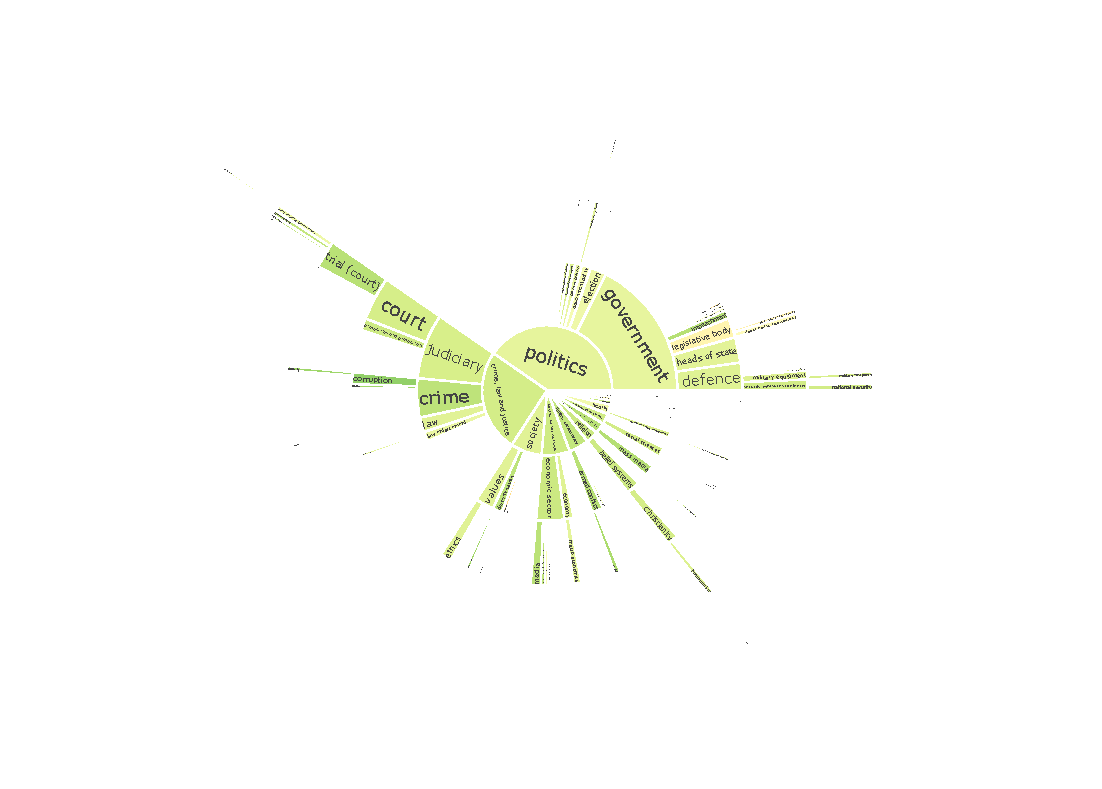
\includegraphics[trim={2.65cm 0cm 0cm 0cm},clip,width=\linewidth]{figures/baly_iptc_weighted_f1_random_bert.pdf}}
    \caption{Random splits}
    \label{fig:baly_iptc_weighted_f1_random_bert}
\end{subfigure}
\begin{subfigure}{0.49\textwidth}
            \centering
    \href{https://martinomensio.github.io/phd-project/figures/baly_iptc_weighted_f1_media_bert.html}{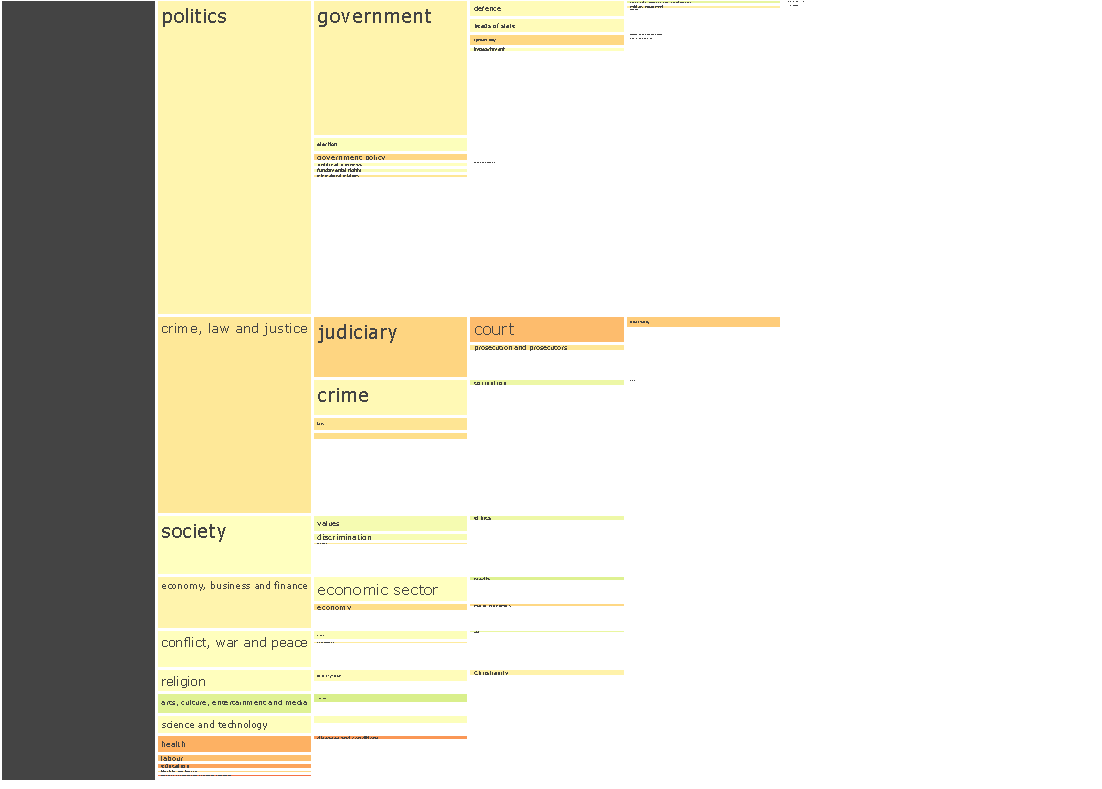
\includegraphics[trim={2.65cm 0cm 0cm 0cm},clip,width=\linewidth]{figures/baly_iptc_weighted_f1_media_bert.pdf}}
    \caption{Media splits}
    \label{fig:baly_iptc_weighted_f1_media_bert}
\end{subfigure}
\caption{F1 across IPTC Media Topics of \texttt{Baly} using \texttt{Baly-baseline (0)}}
    \label{fig:baly_iptc_weighted_f1_bert}
\end{figure}

As Figure~\ref{fig:baly_iptc_weighted_f1_bert} shows,\footnote{Random \url{https://martinomensio.github.io/phd-project/figures/baly_iptc_weighted_f1_random_bert.html} and Media \url{https://martinomensio.github.io/phd-project/figures/baly_iptc_weighted_f1_media_bert.html}} the F1 measures using the baseline BERT features changes across topics and media splits (compare with Table~\ref{tab:results_prop_features_classifier} from the previous chapter).
% \todoAW{You really need to be presenting these results in a way that's comparable across the dissertation.}
First of all, we can notice that the size of the topics is different from the previous figures. This is caused by the splits provided with the dataset that instead of containing a k-fold, they just do a train-test split. Therefore, the figure here represents only the distribution of the test set (for which we have the predictions).

The random split has higher results for almost all the topics, as we discussed in the previous chapter, but it suffers from information leaking (articles from a certain source can appear both in the training and test set, and the models take this as a shortcut).
% \todoAW{Why didn't you just modify the training/test set so that there's no overlap?}
Therefore the more important results are the ones considering the media splits where this problem is solved.

Considering the random splits~\ref{fig:baly_iptc_weighted_f1_random_bert} (macro-F1 $56\%$), the topics where F1 is higher are \texttt{corruption} ($73\%$), \texttt{racism} ($70\%$), \texttt{war} ($68\%$), \texttt{mass-media} ($67\%$), \texttt{Trial} ($66\%$). The ones with the lowest values are \texttt{family} ($39\%$) and \texttt{legislative-body} ($46\%$).

Instead, the media splits~\ref{fig:baly_iptc_weighted_f1_media_bert} have generally lower values (Macro-F1 $40\%$), and the model struggles the most with \texttt{health} ($30\%$), \texttt{court} ($32\%$) and \texttt{labour} ($33\%$).

\begin{figure}[!htbp]
    \centering
	\begin{subfigure}{0.49\textwidth}
            \centering
    \href{https://martinomensio.github.io/phd-project/figures/baly_iptc_weighted_f1_media_propaganda_percentages.html}{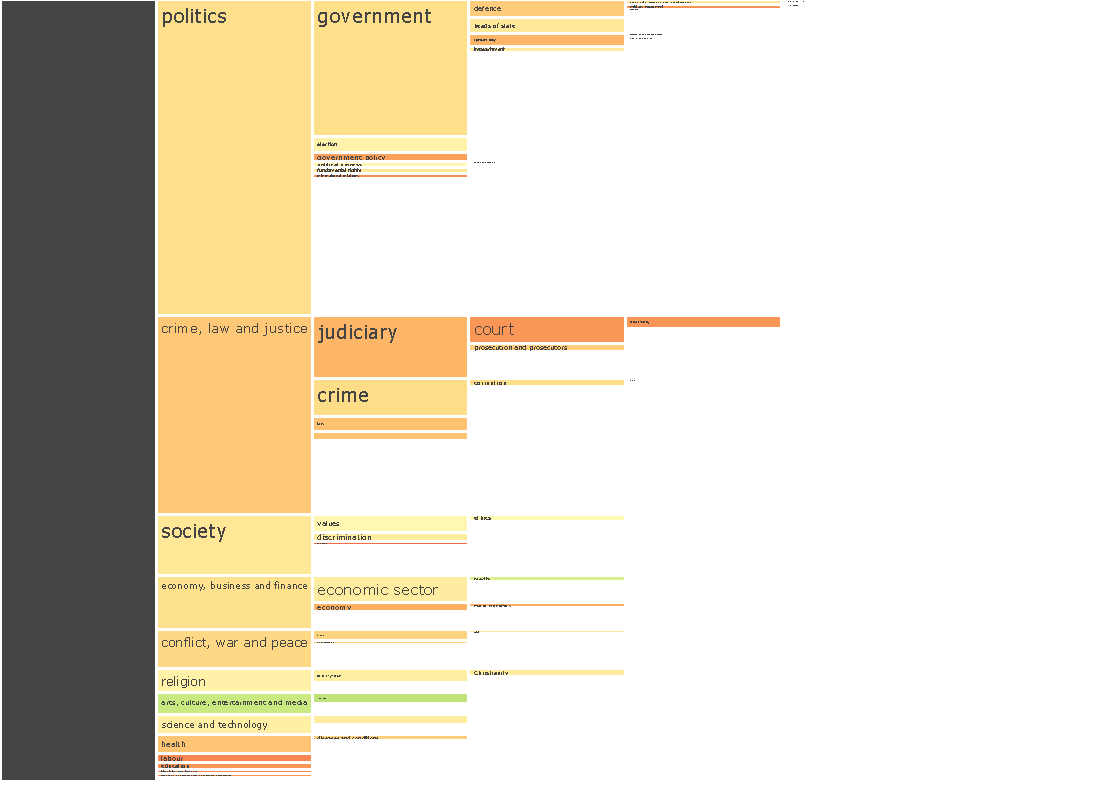
\includegraphics[trim={2.65cm 0cm 0cm 0cm},clip,width=\linewidth]{figures/baly_iptc_weighted_f1_media_propaganda_percentages.pdf}}
    \caption{Propaganda features alone \texttt{(2)}}
    \label{fig:baly_iptc_weighted_f1_media_propaganda_percentages}
\end{subfigure}
\begin{subfigure}{0.49\textwidth}
            \centering
    \href{https://martinomensio.github.io/phd-project/figures/baly_iptc_weighted_f1_media_delta.html}{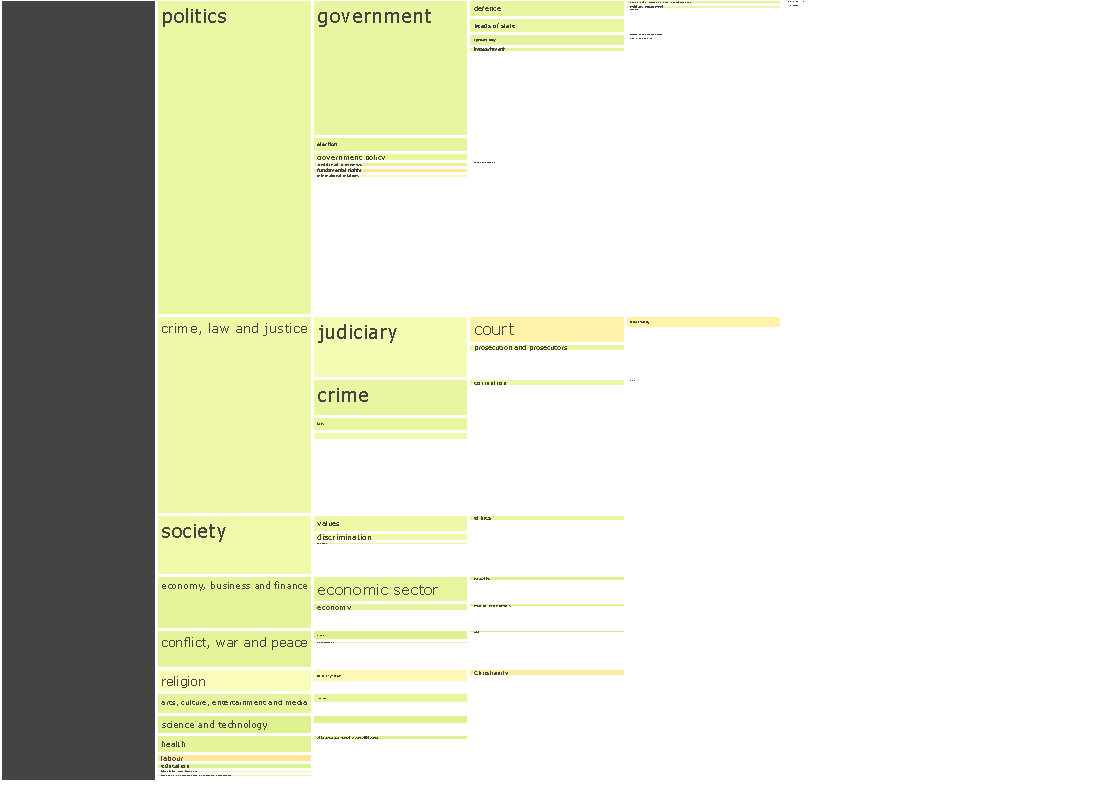
\includegraphics[trim={2.65cm 0cm 0cm 0cm},clip,width=\linewidth]{figures/baly_iptc_weighted_f1_media_delta.pdf}}
    \caption{Relative improvement of \texttt{(0)+(2)}}
    \label{fig:baly_iptc_weighted_f1_media_delta}
\end{subfigure}
\caption{F1 across IPTC Media Topics of \texttt{Baly} using propaganda features \texttt{(2)}}
    \label{fig:baly_iptc_weighted_f1_media_prop}
\end{figure}

% Then show also F1 for the model that uses propaganda features alone
Then we analyse with the same methodology the F1 across topics of the models trained with the propaganda features.
Figure~\ref{fig:baly_iptc_weighted_f1_media_prop} shows the results with two different plots. In~\ref{fig:baly_iptc_weighted_f1_media_propaganda_percentages}, we see that the propaganda features alone have bad results across topics, especially for \texttt{court} ($26\%$). In general, the results are very similar to~\ref{fig:baly_iptc_weighted_f1_media_bert} but all with lower scores.

Instead,~\ref{fig:baly_iptc_weighted_f1_media_delta} shows the relative difference between the rows \texttt{(0)+(2)} and \texttt{(0)} (cfr.Table~\ref{tab:results_prop_features_classifier}).
In other words, it is measuring the effect of adding the propaganda features to the baseline features. Green colour means a relative improvement, while red colour means a degradation of the score for the specific topic.
The overall improvement of $1.37\%$ F1 is focused mostly on \texttt{politics} ($1.2\%$ increase), \texttt{economy-business-and-finance} ($1.9\%$ increase), \texttt{conflict-war-and-peace} ($2.2\%$ increase), \texttt{science-and-technology} ($3.3\%$ increase) and \texttt{health} ($2.0\%$ increase). Instead, some topics are penalised by the addition, such as \texttt{court} ($0.6\%$ decrease), \texttt{belief-systems} ($0.2\%$ decrease).

These results mean that the propaganda features are quite useful to differentiate between Left and Right leaning in topics such as \texttt{politics}, \texttt{economy}, \texttt{conflict-and-science}. For these topics, we saw in the previous sections significant differences between left and right propaganda.
But at the same time, in some topics such as \texttt{court} and \texttt{belief-systems}, which were showing promising statistical differences across leaning, the classifier is not able to use this information to improve the prediction.

\subsection{\statusgreen Predicting Leaning from topics and propaganda}
\label{sec:topic_classifier_propaganda_feature}

For this last experiment, we use the topic as an input feature to try to predict the political leaning of news articles.
%
The idea is that, by using the current topics in the article, the classifier may be able to recognise topic-propaganda associations that we discussed in this chapter, and possibly improve the result of classification.

% - encoding topics
The first step to make this possible is to encode the Media Topics labels into usable features. We are following our previous model architecture, where we first compute features, and then we combine them with a dense layers. The only difference is that in this case, we are using two layers instead of one to be able to capture associations between multiple features.

To encode the topic labels, several options are possible. One-Hot encoding is possible, but does not exploit the hierarchy information. Furthermore, each article is assigned to multiple topics and this would complicate this type of feature. Instead, given that the labels are given in natural language and each Media Topic label is already composed of all the names of the parent topics plus the current subtopic, we decide to use TF-IDF to encode the labels.
For example, for an article that has as labels \texttt{labour > unemployment > unemployment benefits} and \texttt{labour > employment > wage and benefit > social security}, we are first tokenizing and counting the words: \texttt{labour:2}, \texttt{unenmployment:2}, \texttt{benefit:2}, \texttt{employment:1}, \texttt{wage:1}, \texttt{social:1}, \texttt{security:1}. With this counting for all the article, we can then build TF-IDF vectors that are able to be influenced by hierarchy (the terms in the names of higher-level topic are repeated for all the subtopics) and also to solve the multi-label problem.
For TF-IDF we experiment both with feature size 500 and 1000.

% - training classifier
With the topic features computed, we then proceed as in Chapter~\ref{ssec:ps_prop_leaning_classifier}. We consider these added features:

\begin{enumerate}
    \item \texttt{Media Topics TF-IDF 500 (4a)}: TF-IDF with size 500 computed from the topic labels;
    \item \texttt{Media Topics TF-IDF 1000 (4b)}: TF-IDF with size 1000 computed from the topic labels.
\end{enumerate}

We experiment with different features sets, combining topic, propaganda and baseline features.

% \textbf{$\star$69.2994}
\begin{table}[!htbp]
    \centering
   \scriptsize
  %\small
    % \resizebox{\textwidth}{!}{
    \begin{tabular}{l|rr|rr}
        & \multicolumn{2}{c}{\texttt{Random}} & \multicolumn{2}{c}{\texttt{Media}} \\
        Model & F1-Macro & Accuracy & F1-Macro & Accuracy \\
        \hline
        \texttt{Majority} & 17.98 & 36.93 & 17.98 & 36.93 \\
        \texttt{Baly-baseline} (0) & 63.27 & 63.50 & 37.36 & 38.18 \\
        \hline
        \texttt{Prop-Total (1)} & 35.29 & 38.43 & 34.40 & 37.66 \\
        \texttt{Prop-Techniques (2)} & 37.70 & 39.91 & 35.74 & 38.02  \\
        \texttt{Prop-Total-Terms (3a)} & 43.58 & 43.91 & 37.11 & 37.78 \\
        \texttt{Prop-Techniques-Terms (3b)} & 41.97 & 42.56 & 36.06 & 36.78 \\
        \hline
        \texttt{Media Topics TF-IDF 500 (4a)} & 41.01 & 41.98 & 36.60 & 37.76 \\
        \texttt{Media Topics TF-IDF 1000 (4b)} & 41.01 & 41.98 & 36.63 & 37.79 \\
        % \texttt{Prop-words-BERT} (3) & 35.4718 & 48.2387 & 35.4718 & 48.2387 \\
        \hline
        \texttt{(0)+(2)} & \textbf{$\star$63.32} & \textbf{$\star$63.56} & \textbf{37.46} & \textbf{38.25}  \\
        \texttt{(0)+(3a)} & 59.52 & 59.77 & \textbf{38.14} & \textbf{38.89}  \\
        \hline
        \texttt{(2)+(4a)} & 43.22 & 43.89 & \textbf{38.21} & \textbf{39.07}  \\
        \texttt{(2)+(4b)} & 43.18 & 43.86 & \textbf{38.24} & \textbf{39.10}  \\
        \texttt{(2)+(3a)+(4b)} & 45.04 & 45.48 & \textbf{38.07} & \textbf{38.71}  \\
        \texttt{(0)+(3a)+(4a)} & 59.67 & 59.90 & \textbf{38.62} & \textbf{39.42}   \\
        \texttt{(0)+(3a)+(4b)} & 59.64 & 59.86 & \textbf{38.63} & \textbf{39.42}  \\
        \texttt{(0)+(2)+(4a)} & 63.19 & 63.37 & \textbf{37.98} & \textbf{38.79}  \\
        \texttt{(0)+(2)+(4b)} & 63.22 & 63.40 & \textbf{37.97} & \textbf{38.77}  \\
        \texttt{(0)+(2)+(3a)+(4b)} & 59.75 & 59.97 & \textbf{$\star$38.68} & \textbf{$\star$39.46}  \\
        
        
    \end{tabular}
    % }
    \caption{Results Media Topics}
    \label{tab:results_classifier_with_mediatopics}
\end{table}
% \todoAW{Table~\ref{tab:results_classifier_with_mediatopics}: I'm not sure what this shows me. More details needed in the text}

% - results
Table~\ref{tab:results_classifier_with_mediatopics} show the results of the feature sets.
We can see that with the random splits, the features \texttt{(0)+(2)} found in the previous chapter are still the best performers.
Instead, with the media splits, we are able to improve that result by using the topic features.
The best result is achieved in \texttt{(0)+(2)+(3a)+(4b)} which is a combination of BERT baseline \texttt{(0)}, propaganda quantities \texttt{(2)}, propaganda terms \texttt{(3a)} and topic labels \texttt{(4b)}.

The size of the TF-IDF only changes minimally the results, but the size 1000 is better than 500.
The improvement with respect to \texttt{(0)+(2)} is of $1.22\%$, and results significant with a p-value of $1.03 \times 10^{-6}$.

% with respect to baseline
% [18133.  4288.]
%  [ 3825. 10028.]]
% statistic=3825.000, p-value=0.0000002889
% Different proportions of errors (reject H0) SIGNIFICANT
%
% with respect to 0+2
% contingency: [[18155.  4242.]
%  [ 3803. 10074.]]
% statistic=3803.000, p-value=0.0000010373 

The significance of these results means that \emph{using the topics in addition to propaganda features is useful to classify political leaning}. The many topic-techniques associations that we discovered previously enable the classifier to improve slightly the predictions.
%
We have, although, the limitation that the net increase of F1 is still minimal ($1.22\%$).

\section{\statusgreen Discussions}
\label{sec:topic_discussion}

The main findings of this chapter are:

\begin{enumerate}
    \item We need fine-grained topic to be more able to see differences. The coarse topics show similar propaganda across topics and leanings. The more we use fine-grained topics, the more differences we are able to see.
    Although, the more we use specific and narrow topics, the less articles we have into each group. This causes the results to lose statistical significance when the topics are too narrow.
    % we lose support\todoHA{??} (fewer articles specific to the topics, and the filtering becomes too narrow).
    We need a tradeoff between granularity (high, to see good differences) and number of articles per topic (significance of results).
    \item Certain topics have more propaganda on a specific leaning. This happens with topics that are more important from the considered point of view, or where the considered leaning is currently against the status quo.
    \item The distribution of propaganda techniques is very similar across leanings for most of the topics (relative ratio of the quantity of techniques between themselves). Combined with the previous finding, it means that the quantities of the techniques scale proportionally across leanings in most of the topics.
    \item The terms of propaganda can be quite different across political leaning in certain topics. For some of these topics, they already have an imbalance of total quantity (e.g. Left has more propaganda than Right), for some others, the quantity is very similar, but they differ in the terms used.
    \item For a set of topics, it is easier to classify correctly the political leaning than in others. The easiest topics for recognising the leaning are the ones that are more polarising.
    \item Adding propaganda features to the baseline model has a positive impact on prediction metrics on major topics, while for other topics instead, it has negative impacts.
    \item Encoding the topic information and using it as a feature helps to increase the prediction metrics of a leaning classifier. The improvements are small but significant.
\end{enumerate}


The answers to the subquestions for this chapter are the following:

\begin{enumerate}[label={\textbf{RQ4.\arabic*:}},leftmargin=2cm]
    \item \emph{How does detected propaganda differ across polarising versus neutral topics?} We identified topics that contain more propaganda (polarising) than others. What does not change generally is the proportion between the techniques used. \texttt{Loaded\_Language} is always the most common, and there are a few exceptions where a specific technique is used in a certain topic outside its usual range.
    \item \emph{How does detected propaganda differ across political leaning in polarising and neutral topics?} When comparing across political leaning, some topics have a higher quantity of propaganda on a specific leaning (finding 2 above). The internal proportion of techniques is preserved (finding 3), but the specific terms have substantial differences (finding 4).
    \item \textit{What are the effects of combining the propaganda features with the topic features, to recognise the leaning of a news article?} Adding the topic features to the propaganda features is useful to recognise the leaning of news articles, but not for all the topics. The small improvements show statistical significance.
\end{enumerate}

After this discussion, we can answer our RQ4: \emph{How does the use of propaganda differ across topics, and to what extent could this help determine the political leaning of articles?}
Propaganda changes significantly across topics, especially when considering the terms used. Using the topic as an input feature for classifying political leaning is beneficial if used together with the propaganda features. The reason is that we can exploit some associations of topics and propaganda that make it easier to recognise the political leaning of news articles.


\section{Conclusions}
\label{sec:topic_conclusion}

This chapter investigated the importance of the topics in our work about propaganda.
First of all, we have been able to refine and select a methodology to perform a comparative analysis across topics and leanings. With hierarchical topics we are able to find interesting results at multiple levels of granularity.
We discovered several associations of topics and propaganda, and we have a much clearer view of how these different variables interconnect with each other.
% \todoHA{What else can we use this knowledge for?}
This knowledge can be used for refining classification models for certain topics, or also to
% explore the connections with other phenomena such as
investigate and possibly improve the detection of propaganda in specific topics, to create more diverse datasets.

As possible limitations of the methods used, we have external factors, such as the propaganda detection model or the topic detection model (TextRazor). But we have as well internal factors, such as the specific usage of the topic scores, or the encoding of the labels with TF-IDF that could have been done differently.

Another limitation is the usage of a single dataset to perform the analysis.
In this chapter, we used only the \texttt{baly} dataset because it is smaller and easier to handle from the computational point of view. We have also extracted the topic features for the \texttt{NELA-GT} dataset used in the previous chapter, but the large size requirements are more difficult to satisfy. It would be interesting to see if the results obtained also generalise to this second dataset and potentially other datasets.
